\documentclass[12pt,spanish]{article}
\usepackage[spanish]{babel}
\usepackage{graphicx}
\usepackage{multirow}
\usepackage{float}
\usepackage{enumitem}
\usepackage[hidelinks]{hyperref}
\usepackage{array}
\graphicspath{ {../../../../LaTeX/img/} {../diagramas/} {../img/} {../../LaTeX/img/}}
\usepackage[table]{xcolor}
\selectlanguage{spanish}
\usepackage[utf8]{inputenc}
\usepackage{graphicx}
\usepackage[ddmmyy]{datetime}
\usepackage[a4paper,left=3cm,right=2cm,top=2.5cm,bottom=2.5cm]{geometry}
\makeindex

\begin{document}
\begin{titlepage}

\newlength{\centeroffset}
\setlength{\centeroffset}{-0.5\oddsidemargin}
\addtolength{\centeroffset}{0.5\evensidemargin}
\thispagestyle{empty}

\noindent\hspace*{\centeroffset}\begin{minipage}{\textwidth}

\centering

\includegraphics[width=0.9\textwidth]{logo_ugr.jpg}\\[1.4cm]

\textsc{ \Large Fundamentos de Ingeniería del Software\\[0.2cm]}
\textsc{GRADO EN INGENIERÍA INFORMÁTICA}\\[1cm]

{\Huge\bfseries Práctica 2. Modelos de casos de uso\\
}
\noindent\rule[-1ex]{\textwidth}{3pt}\\[3.5ex]
{\large\bfseries Segunda parte}
\end{minipage}

\vspace{2.5cm}
\noindent\hspace*{\centeroffset}
\begin{minipage}{\textwidth}
\centering

\textbf{Autores}\\ {José Baena Cobos \\ José Miguel Pelegrina Pelegrina\\Carlos Sánchez Páez}\\[2.5ex]

\includegraphics[width=0.3\textwidth]{etsiit_logo.png}\\[0.1cm]
\vspace{1.5cm}

\includegraphics[width=0.2\textwidth]{lsi.png}\\[0.1cm]
\vspace{1cm}
\textsc{Escuela Técnica Superior de Ingenierías Informática y de Telecomunicación}\\
\vspace{1cm}
\textsc{Curso 2017-2018}
\end{minipage}
\end{titlepage}
\tableofcontents
\thispagestyle{empty}
\listoffigures
\listoftables
\setcounter{page}{1}
%%%%%%%%%%%%%%%%%%%%%%%%Comienzo del documento%%%%%%%%%%%%%%%%%%%%%%%%%%%%%%%

\section{Diagrama de actividad}
\begin{figure}[H]
\centering
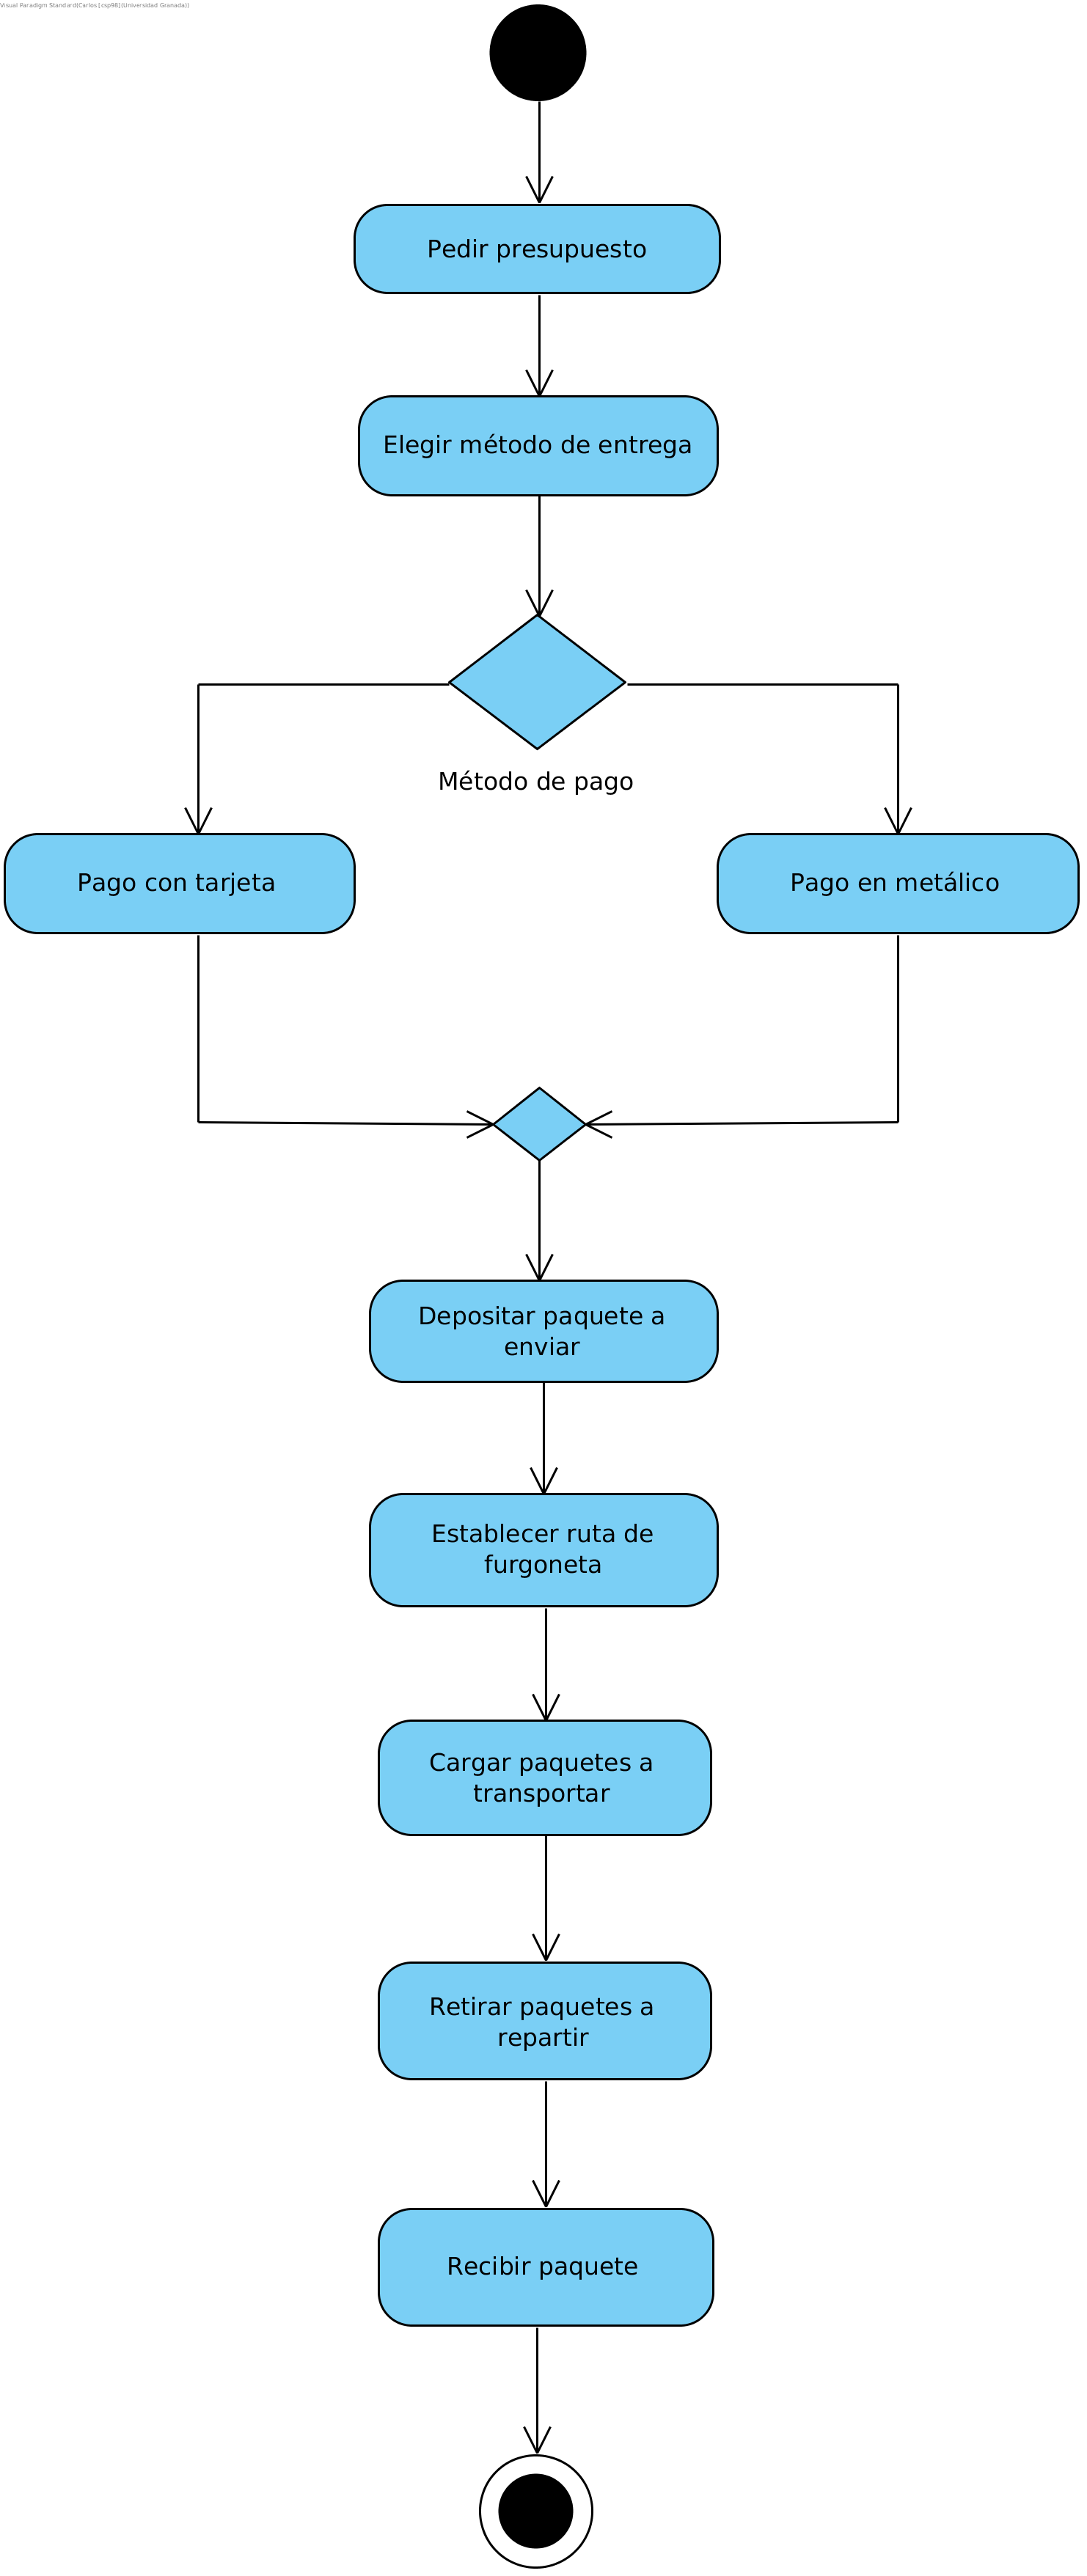
\includegraphics[scale=0.75]{actividad.png}
\caption{Diagrama de actividades.}
\end{figure}

\section{Descripción de casos de uso a nivel extendido}

\newcounter{contadorCU}
\setcounter{contadorCU}{1}


%%%%ALTA EMPLEADO%%%%

\begin{table}[H]
\centering
\begin{tabular}{|m{3cm}|m{4cm}|m{2cm}|m{2cm}|m{2cm}|m{1cm}|}
\hline
\textbf{Caso de uso} &  \multicolumn{4}{m{8cm}|}{Alta empleado} \vline &  \cellcolor{gray!40}CU\arabic{contadorCU}  \stepcounter{contadorCU}
\\
\hline
\textbf{Actores} & \multicolumn{5}{m{8cm}|}{Empleado y oficinista} \\
\hline
\textbf{Tipo} & \multicolumn{5}{m{8cm}|}{Real} \\
\hline
\textbf{Referencias} &\multicolumn{5}{m{8cm}|}{-} \\
\hline
\textbf{Precondición} & \multicolumn{5}{m{8cm}|}{-} \\
\hline
\textbf{Postcondición} & \multicolumn{5}{m{8cm}|}{El nuevo empleado podrá acceder al sistema mediante un login} \\
\hline
\textbf{Autor} & Carlos Sánchez Páez & \textbf{Fecha} & 08/04/2018 & \textbf{Versión} & 2.0 \\
\hline
\end{tabular}

\vspace{1cm}

\begin{tabular}{|m{16.2cm}|}
\hline
\textbf{Propósito} \\
\hline
Poder incorporar a un nuevo empleado al sistema. \\
\hline
\end{tabular}

\vspace{1cm}

\begin{tabular}{|m{16.2cm}|}
\hline
\textbf{Resumen} \\
\hline
Un nuevo empleado pasará a formar parte de la empresa. Podrá acceder al sistema con sus credenciales y tendrá unos privilegios determinados. \\
\hline
\end{tabular}

\vspace{1cm}

\begin{tabular}{|m{4pt}|m{7.33cm}|m{4pt}|m{7.33cm}|}
\hline
\multicolumn{4}{|c|}{\textbf{Curso normal}} \\
\hline
\textbf{1} & El oficinista pide al nuevo empleado sus datos y los introduce en el sistema. & \textbf{2} & El sistema comprueba que los datos sean válidos y no existan ya. \\
\hline
\textbf{3} &  & \textbf{4} & El sistema imprime los credenciales de acceso del nuevo empleado. \\
\hline
\textbf{5} & El oficinista da los credenciales al empleado & \textbf{6} &  \\
\hline
\end{tabular}

\vspace{1cm}

\begin{tabular}{|m{10pt}|m{7.15cm}|m{10pt}|m{7.15cm}|}
\hline
\multicolumn{4}{|m{16.2cm}|}{\textbf{Cursos alternos}} \\
\hline
\multicolumn{4}{|m{16.2cm}|}{\textbf{2a) Los datos no son correctos}} \\
\hline
\multicolumn{4}{|m{16.2cm}|}{El sistema informa del error y vuelve a solicitar los datos.} \\
\hline
\end{tabular}

\vspace{1cm}

\begin{tabular}{|m{3.72cm}|m{3.72cm}|m{3.72cm}|m{3.72cm}|}
\hline
\multicolumn{4}{|c|}{\textbf{Otros datos}} \\
\hline
\textbf{Frecuencia esperada} & Media (tres veces al mes) & \textbf{Rendimiento} & - \\
\hline
\textbf{Importancia} & Alta & \textbf{Urgencia} & Máxima \\
\hline
\textbf{Estado} & Implementado & \textbf{Estabilidad} & Alta \\
\hline
\end{tabular}

\vspace{1cm}

\begin{tabular}{|m{16.2cm}|}
\hline
\textbf{Comentarios} \\
\hline
- \\
\hline
\end{tabular}

\caption{Alta empleado}

\end{table}


%%%%%%%%BAJA EMPLEADO%%%%%

\begin{table}[H]
\centering
\begin{tabular}{|m{3cm}|m{4cm}|m{2cm}|m{2cm}|m{2cm}|m{1cm}|}
\hline
\textbf{Caso de uso} &  \multicolumn{4}{m{8cm}|}{Baja empleado} \vline &  \cellcolor{gray!40}CU\arabic{contadorCU}  \stepcounter{contadorCU}
\\
\hline
\textbf{Actores} & \multicolumn{5}{m{8cm}|}{Empleado y oficinista} \\
\hline
\textbf{Tipo} & \multicolumn{5}{m{8cm}|}{Real} \\
\hline
\textbf{Referencias} &\multicolumn{5}{m{8cm}|}{-} \\
\hline
\textbf{Precondición} & \multicolumn{5}{m{8cm}|}{El empleado debe estar dado de alta en el sistema.} \\
\hline
\textbf{Postcondición} & \multicolumn{5}{m{8cm}|}{El empleado ya no podrá acceder al sistema.} \\
\hline
\textbf{Autor} & Carlos Sánchez Páez & \textbf{Fecha} & 08/04/2018 & \textbf{Versión} & 2.0 \\
\hline
\end{tabular}

\vspace{1cm}

\begin{tabular}{|m{16.2cm}|}
\hline
\textbf{Propósito} \\
\hline
Eliminar los datos de un empleado. \\
\hline
\end{tabular}

\vspace{1cm}

\begin{tabular}{|m{16.2cm}|}
\hline
\textbf{Resumen} \\
\hline
Los datos del empleado son eliminados del sistema, perdiendo todo el acceso al mismo. \\
\hline
\end{tabular}

\vspace{1cm}

\begin{tabular}{|m{4pt}|m{7.33cm}|m{4pt}|m{7.33cm}|}
\hline
\multicolumn{4}{|c|}{\textbf{Curso normal}} \\
\hline
\textbf{1} & El oficinista solicita al empleado sus datos y los introduce en el sistema. & \textbf{2} & El sistema verifica los datos y solicita confirmación \\
\hline
\textbf{3} & El oficinista confirma la baja del empleado.  & \textbf{4} & El sistema elimina los datos del empleado. \\
\hline
\end{tabular}

\vspace{1cm}

\begin{tabular}{|m{10pt}|m{7.15cm}|m{10pt}|m{7.15cm}|}
\hline
\multicolumn{4}{|m{16.2cm}|}{\textbf{Cursos alternos}} \\
\hline
\multicolumn{4}{|m{16.2cm}|}{\textbf{2a) Los datos no son válidos}} \\
\hline
\multicolumn{4}{|m{16.2cm}|}{El sistema informa del error y solicita que los datos se vuelvan a introducir.} \\
\hline
\end{tabular}

\vspace{1cm}

\begin{tabular}{|m{3.72cm}|m{3.72cm}|m{3.72cm}|m{3.72cm}|}
\hline
\multicolumn{4}{|c|}{\textbf{Otros datos}} \\
\hline
\textbf{Frecuencia esperada} & Baja (una vez cada dos meses) & \textbf{Rendimiento} & - \\
\hline
\textbf{Importancia} & Alta & \textbf{Urgencia} & Máxima \\
\hline
\textbf{Estado} & En desarrollo & \textbf{Estabilidad} & Alta \\
\hline
\end{tabular}

\vspace{1cm}

\begin{tabular}{|m{16.2cm}|}
\hline
\textbf{Comentarios} \\
\hline
- \\
\hline
\end{tabular}

\caption{Baja empleado}

\end{table}

%%%%%%%%%%MODIFICAR DATOS PERSONALES EMPLEADO%%%%%%%%%%%	
\begin{table}[H]
\centering
\begin{tabular}{|m{3cm}|m{4cm}|m{2cm}|m{2cm}|m{2cm}|m{1cm}|}
\hline
\textbf{Caso de uso} &  \multicolumn{4}{m{8cm}|}{Modificar datos personales del empleado} \vline &  \cellcolor{gray!40}CU\arabic{contadorCU}  \stepcounter{contadorCU}
\\
\hline
\textbf{Actores} & \multicolumn{5}{m{8cm}|}{Empleado} \\
\hline
\textbf{Tipo} & \multicolumn{5}{m{8cm}|}{} \\
\hline
\textbf{Referencias} &\multicolumn{5}{m{8cm}|}{} \\
\hline
\textbf{Precondición} & \multicolumn{5}{m{8cm}|}{El empleado debe estar registrado en el sistema.} \\
\hline
\textbf{Postcondición} & \multicolumn{5}{m{8cm}|}{Los datos antiguos del empleado son eliminados.} \\
\hline
\textbf{Autor} & Carlos Sánchez Páez & \textbf{Fecha} & 08/04/2018 & \textbf{Versión} & 2.0 \\
\hline
\end{tabular}

\vspace{1cm}

\begin{tabular}{|m{16.2cm}|}
\hline
\textbf{Propósito} \\
\hline
Actualizar los datos de un empleado. \\
\hline
\end{tabular}

\vspace{1cm}

\begin{tabular}{|m{16.2cm}|}
\hline
\textbf{Resumen} \\
\hline
Sustituir datos antiguos de un empleado por otros más actualizados. \\
\hline
\end{tabular}

\vspace{1cm}

\begin{tabular}{|m{4pt}|m{7.33cm}|m{4pt}|m{7.33cm}|}
\hline
\multicolumn{4}{|c|}{\textbf{Curso normal}} \\
\hline
\textbf{1} & El empleado se identifica en el sistema. & \textbf{2} & El sistema valida los datos. \\
\hline
\textbf{3} & El empleado solicita modificar los datos. & \textbf{4} & El sistema muestra los datos actuales. \\
\hline
\textbf{5} & El empleado introduce los nuevos datos y confirma el cambio. & \textbf{6} & El sistema actualiza los datos. \\
\hline
\end{tabular}

\vspace{1cm}

\begin{tabular}{|m{10pt}|m{7.15cm}|m{10pt}|m{7.15cm}|}
\hline
\multicolumn{4}{|m{16.2cm}|}{\textbf{Cursos alternos}} \\
\hline
\multicolumn{4}{|m{16.2cm}|}{\textbf{2a) Los datos no son válidos}} \\
\hline
\multicolumn{4}{|m{16.2cm}|}{El sistema informa del error y solicita que los datos se vuelvan a introducir.} \\
\hline
\end{tabular}

\vspace{1cm}

\begin{tabular}{|m{3.72cm}|m{3.72cm}|m{3.72cm}|m{3.72cm}|}
\hline
\multicolumn{4}{|c|}{\textbf{Otros datos}} \\
\hline
\textbf{Frecuencia esperada} & Media (una vez al mes) & \textbf{Rendimiento} & - \\
\hline
\textbf{Importancia} & Alta & \textbf{Urgencia} & Alta \\
\hline
\textbf{Estado} & En desarrollo & \textbf{Estabilidad} & Alta \\
\hline
\end{tabular}

\vspace{1cm}

\begin{tabular}{|m{16.2cm}|}
\hline
\textbf{Comentarios} \\
\hline
- \\
\hline
\end{tabular}

\caption{Modificar datos personales del empleado}

\end{table}

%%%%%%%%%%%%CAMBIAR DISPONIBILIDAD%%%%%%%%%%%%

\begin{table}[H]
\centering
\begin{tabular}{|m{3cm}|m{4cm}|m{2cm}|m{2cm}|m{2cm}|m{1cm}|}
\hline
\textbf{Caso de uso} &  \multicolumn{4}{m{8cm}|}{Cambiar disponibilidad} \vline &  \cellcolor{gray!40}CU\arabic{contadorCU}  \stepcounter{contadorCU}
\\
\hline
\textbf{Actores} & \multicolumn{5}{m{8cm}|}{Oficinista.} \\
\hline
\textbf{Tipo} & \multicolumn{5}{m{8cm}|}{Real.} \\
\hline
\textbf{Referencias} &\multicolumn{5}{m{8cm}|}{-} \\
\hline
\textbf{Precondición} & \multicolumn{5}{m{8cm}|}{El oficinista debe estar dado de alta en el sistema.} \\
\hline
\textbf{Postcondición} & \multicolumn{5}{m{8cm}|}{-} \\
\hline
\textbf{Autor} & Carlos Sánchez Páez & \textbf{Fecha} & 08/04/2018 & \textbf{Versión} & 2.0 \\
\hline
\end{tabular}

\vspace{1cm}

\begin{tabular}{|m{16.2cm}|}
\hline
\textbf{Propósito} \\
\hline
Cambiar la disponibilidad del oficinista. \\
\hline
\end{tabular}

\vspace{1cm}

\begin{tabular}{|m{16.2cm}|}
\hline
\textbf{Resumen} \\
\hline
El oficinista actualiza sus datos de disponibilidad. \\
\hline
\end{tabular}

\vspace{1cm}

\begin{tabular}{|m{4pt}|m{7.33cm}|m{4pt}|m{7.33cm}|}
\hline
\multicolumn{4}{|c|}{\textbf{Curso normal}} \\
\hline
\textbf{1} & El oficinista se identifica en el sistema. & \textbf{2} & El sistema valida los datos. \\
\hline
\textbf{3} & El oficinista solicita modificar su disponibilidad. & \textbf{4} & El sistema muestra los datos actuales. \\
\hline
\textbf{5} & El oficinista introduce los nuevos datos y confirma el cambio. & \textbf{6} & El sistema actualiza los datos. \\
\hline
\end{tabular}

\vspace{1cm}

\begin{tabular}{|m{10pt}|m{7.15cm}|m{10pt}|m{7.15cm}|}
\hline
\multicolumn{4}{|m{16.2cm}|}{\textbf{Cursos alternos}} \\
\hline
\multicolumn{4}{|m{16.2cm}|}{\textbf{2a) Los datos no son válidos}} \\
\hline
\multicolumn{4}{|m{16.2cm}|}{El sistema informa del error y solicita que los datos se vuelvan a introducir.} \\
\hline
\end{tabular}

\vspace{1cm}

\begin{tabular}{|m{3.72cm}|m{3.72cm}|m{3.72cm}|m{3.72cm}|}
\hline
\multicolumn{4}{|c|}{\textbf{Otros datos}} \\
\hline
\textbf{Frecuencia esperada} & Media (una vez al mes) & \textbf{Rendimiento} & - \\
\hline
\textbf{Importancia} & Alta & \textbf{Urgencia} & Alta \\
\hline
\textbf{Estado} & En desarrollo & \textbf{Estabilidad} & Alta \\
\hline
\end{tabular}

\vspace{1cm}

\begin{tabular}{|m{16.2cm}|}
\hline
\textbf{Comentarios} \\
\hline
- \\
\hline
\end{tabular}

\caption{Cambiar disponibilidad}

\end{table}

%%%%%%%%%%%%%%ASIGNAR RUTA DE TRANSPORTE%%%%%%%%%%

\begin{table}[H]
\centering
\begin{tabular}{|m{3cm}|m{4cm}|m{2cm}|m{2cm}|m{2cm}|m{1cm}|}
\hline
\textbf{Caso de uso} &  \multicolumn{4}{m{8cm}|}{Asignar ruta de transporte} \vline &  \cellcolor{gray!40}CU\arabic{contadorCU}  \stepcounter{contadorCU}
\\
\hline
\textbf{Actores} & \multicolumn{5}{m{8cm}|}{Conductor y oficinista.} \\
\hline
\textbf{Tipo} & \multicolumn{5}{m{8cm}|}{Real.} \\
\hline
\textbf{Referencias} &\multicolumn{5}{m{8cm}|}{-} \\
\hline
\textbf{Precondición} & \multicolumn{5}{m{8cm}|}{Los actores deben estar dados de alta en el sistema.} \\
\hline
\textbf{Postcondición} & \multicolumn{5}{m{8cm}|}{-} \\
\hline
\textbf{Autor} & Carlos Sánchez Páez & \textbf{Fecha} & 08/04/2018 & \textbf{Versión} & 2.0 \\
\hline
\end{tabular}

\vspace{1cm}

\begin{tabular}{|m{16.2cm}|}
\hline
\textbf{Propósito} \\
\hline
Establecer destinos a visitar por el conductor. \\
\hline
\end{tabular}

\vspace{1cm}

\begin{tabular}{|m{16.2cm}|}
\hline
\textbf{Resumen} \\
\hline
Se le asigna al conductor una serie de destinos que tendrá que visitar en su próxima jornada laboral. \\
\hline
\end{tabular}

\vspace{1cm}

\begin{tabular}{|m{4pt}|m{7.33cm}|m{4pt}|m{7.33cm}|}
\hline
\multicolumn{4}{|c|}{\textbf{Curso normal}} \\
\hline
\textbf{1} & El oficinista introduce los datos del conductor en el sistema. & \textbf{2} & El sistema valida los datos. \\
\hline
\textbf{3} & El oficinista solicita la ruta de transporte & \textbf{4} & El sistema muestra la ruta. \\
\hline
\textbf{5} & El oficinista informa de la ruta al conductor. & \textbf{6} &  \\
\hline
\end{tabular}

\vspace{1cm}

\begin{tabular}{|m{10pt}|m{7.15cm}|m{10pt}|m{7.15cm}|}
\hline
\multicolumn{4}{|m{16.2cm}|}{\textbf{Cursos alternos}} \\
\hline
\multicolumn{4}{|m{16.2cm}|}{\textbf{2a) Los datos no son válidos}} \\
\hline
\multicolumn{4}{|m{16.2cm}|}{El sistema informa del error y solicita que los datos se vuelvan a introducir.} \\
\hline
\multicolumn{4}{|m{16.2cm}|}{\textbf{3a) No se han introducido los destinos a visitar}} \\
\hline
\multicolumn{4}{|m{16.2cm}|}{El sistema informa del error y solicita que los datos se introduzcan.} \\
\hline
\end{tabular}

\vspace{1cm}

\begin{tabular}{|m{3.72cm}|m{3.72cm}|m{3.72cm}|m{3.72cm}|}
\hline
\multicolumn{4}{|c|}{\textbf{Otros datos}} \\
\hline
\textbf{Frecuencia esperada} & Alta (a diario) & \textbf{Rendimiento} & - \\
\hline
\textbf{Importancia} & Extrema & \textbf{Urgencia} & Máxima \\
\hline
\textbf{Estado} & Implementado & \textbf{Estabilidad} & Alta \\
\hline
\end{tabular}

\vspace{1cm}

\begin{tabular}{|m{16.2cm}|}
\hline
\textbf{Comentarios} \\
\hline
- \\
\hline
\end{tabular}

\caption{Asignar ruta de transporte}

\end{table}


%%%%%%%%CONSULTAR ESTADO DE CONDUCTOR%%%%%%%%%%%

\begin{table}[H]
\centering
\begin{tabular}{|m{3cm}|m{4cm}|m{2cm}|m{2cm}|m{2cm}|m{1cm}|}
\hline
\textbf{Caso de uso} &  \multicolumn{4}{m{8cm}|}{Consultar estado de conductor} \vline &  \cellcolor{gray!40}CU\arabic{contadorCU}  \stepcounter{contadorCU}
\\
\hline
\textbf{Actores} & \multicolumn{5}{m{8cm}|}{Oficinista} \\
\hline
\textbf{Tipo} & \multicolumn{5}{m{8cm}|}{Real} \\
\hline
\textbf{Referencias} &\multicolumn{5}{m{8cm}|}{-} \\
\hline
\textbf{Precondición} & \multicolumn{5}{m{8cm}|}{El conductor debe estar dado de alta en el sistema.} \\
\hline
\textbf{Postcondición} & \multicolumn{5}{m{8cm}|}{-} \\
\hline
\textbf{Autor} & Carlos Sánchez Páez & \textbf{Fecha} & 08/04/2018 & \textbf{Versión} & 2.0 \\
\hline
\end{tabular}

\vspace{1cm}

\begin{tabular}{|m{16.2cm}|}
\hline
\textbf{Propósito} \\
\hline
Ver información relativa al conductor. \\
\hline
\end{tabular}

\vspace{1cm}

\begin{tabular}{|m{16.2cm}|}
\hline
\textbf{Resumen} \\
\hline
El oficinista podrá obtener información sobre el conductor (destinos realizados/pendientes, furgoneta asociada, etc.) \\
\hline
\end{tabular}

\vspace{1cm}

\begin{tabular}{|m{4pt}|m{7.33cm}|m{4pt}|m{7.33cm}|}
\hline
\multicolumn{4}{|c|}{\textbf{Curso normal}} \\
\hline
\textbf{1} & El oficinista introduce los datos del conductor en el sistema. & \textbf{2} & El sistema valida los datos. \\
\hline
\textbf{3} & El oficinista solicita la información requerida. & \textbf{4} & El sistema muestra la información. \\
\hline
\end{tabular}

\vspace{1cm}

\begin{tabular}{|m{10pt}|m{7.15cm}|m{10pt}|m{7.15cm}|}
\hline
\multicolumn{4}{|m{16.2cm}|}{\textbf{Cursos alternos}} \\
\hline
\multicolumn{4}{|m{16.2cm}|}{\textbf{2a) Los datos no son válidos}} \\
\hline
\multicolumn{4}{|m{16.2cm}|}{El sistema informa del error y solicita que los datos se vuelvan a introducir.} \\
\hline
\end{tabular}

\vspace{1cm}

\begin{tabular}{|m{3.72cm}|m{3.72cm}|m{3.72cm}|m{3.72cm}|}
\hline
\multicolumn{4}{|c|}{\textbf{Otros datos}} \\
\hline
\textbf{Frecuencia esperada} & Alta (a diario) & \textbf{Rendimiento} & - \\
\hline
\textbf{Importancia} & Extrema & \textbf{Urgencia} & Máxima \\
\hline
\textbf{Estado} & En desarrollo & \textbf{Estabilidad} & Alta \\
\hline
\end{tabular}

\vspace{1cm}

\begin{tabular}{|m{16.2cm}|}
\hline
\textbf{Comentarios} \\
\hline
- \\
\hline
\end{tabular}

\caption{Consultar estado de conductor}

\end{table}

%%%%%%%%%%ALTA SUCURSAL%%%%%%%%%%

\begin{table}[H]
\centering
\begin{tabular}{|m{3cm}|m{4cm}|m{2cm}|m{2cm}|m{2cm}|m{1cm}|}
\hline
\textbf{Caso de uso} &  \multicolumn{4}{m{8cm}|}{Alta sucursal} \vline &  \cellcolor{gray!40}CU\arabic{contadorCU}  \stepcounter{contadorCU}
\\
\hline
\textbf{Actores} & \multicolumn{5}{m{8cm}|}{Oficinista} \\
\hline
\textbf{Tipo} & \multicolumn{5}{m{8cm}|}{Real} \\
\hline
\textbf{Referencias} &\multicolumn{5}{m{8cm}|}{CU8,CU9} \\
\hline
\textbf{Precondición} & \multicolumn{5}{m{8cm}|}{-} \\
\hline
\textbf{Postcondición} & \multicolumn{5}{m{8cm}|}{-} \\
\hline
\textbf{Autor} & Carlos Sánchez Páez & \textbf{Fecha} & 08/04/2018 & \textbf{Versión} & 2.0 \\
\hline
\end{tabular}

\vspace{1cm}

\begin{tabular}{|m{16.2cm}|}
\hline
\textbf{Propósito} \\
\hline
Incorporar una nueva sucursal al sistema. \\
\hline
\end{tabular}

\vspace{1cm}

\begin{tabular}{|m{16.2cm}|}
\hline
\textbf{Resumen} \\
\hline
Una nueva sucursal pasará a formar parte de la empresa, pudiendo acceder sus empleados al sistema. \\
\hline
\end{tabular}

\vspace{1cm}

\begin{tabular}{|m{4pt}|m{7.33cm}|m{4pt}|m{7.33cm}|}
\hline
\multicolumn{4}{|c|}{\textbf{Curso normal}} \\
\hline
\textbf{1} & El oficinista inicia el proceso de alta. & \textbf{2} & El sistema ofrece un formulario a rellenar. \\
\hline
\textbf{3} & El oficinista rellena el formulario. & \textbf{4} & El sistema comprueba los datos. \\
\hline
\textbf{5} & & \textbf{6} & incluir(CU8, alta oficina) \\
\hline
\end{tabular}

\vspace{1cm}

\begin{tabular}{|m{10pt}|m{7.15cm}|m{10pt}|m{7.15cm}|}
\hline
\multicolumn{4}{|m{16.2cm}|}{\textbf{Cursos alternos}} \\
\hline
\multicolumn{4}{|m{16.2cm}|}{\textbf{4a) Los datos no son válidos}} \\
\hline
\multicolumn{4}{|m{16.2cm}|}{El sistema informa del error y solicita que los datos se vuelvan a introducir.} \\
\hline
\end{tabular}

\vspace{1cm}

\begin{tabular}{|m{3.72cm}|m{3.72cm}|m{3.72cm}|m{3.72cm}|}
\hline
\multicolumn{4}{|c|}{\textbf{Otros datos}} \\
\hline
\textbf{Frecuencia esperada} & Media (una vez al trimestre) & \textbf{Rendimiento} & - \\
\hline
\textbf{Importancia} & Alta & \textbf{Urgencia} & Media \\
\hline
\textbf{Estado} & En desarrollo & \textbf{Estabilidad} & Alta \\
\hline
\end{tabular}

\vspace{1cm}

\begin{tabular}{|m{16.2cm}|}
\hline
\textbf{Comentarios} \\
\hline
- \\
\hline
\end{tabular}

\caption{Alta sucursal}

\end{table}


%%%%%%%%%ALTA OFICINA%%%%%%

\begin{table}[H]
\centering
\begin{tabular}{|m{3cm}|m{4cm}|m{2cm}|m{2cm}|m{2cm}|m{1cm}|}
\hline
\textbf{Caso de uso} &  \multicolumn{4}{m{8cm}|}{Alta oficina} \vline &  \cellcolor{gray!40}CU\arabic{contadorCU}  \stepcounter{contadorCU}
\\
\hline
\textbf{Actores} & \multicolumn{5}{m{8cm}|}{Oficinista} \\
\hline
\textbf{Tipo} & \multicolumn{5}{m{8cm}|}{Real} \\
\hline
\textbf{Referencias} &\multicolumn{5}{m{8cm}|}{-} \\
\hline
\textbf{Precondición} & \multicolumn{5}{m{8cm}|}{-} \\
\hline
\textbf{Postcondición} & \multicolumn{5}{m{8cm}|}{-} \\
\hline
\textbf{Autor} & Carlos Sánchez Páez & \textbf{Fecha} & 08/04/2018 & \textbf{Versión} & 2.0 \\
\hline
\end{tabular}

\vspace{1cm}

\begin{tabular}{|m{16.2cm}|}
\hline
\textbf{Propósito} \\
\hline
Dar de alta una oficina en el sistema. \\
\hline
\end{tabular}

\vspace{1cm}

\begin{tabular}{|m{16.2cm}|}
\hline
\textbf{Resumen} \\
\hline
La oficina pasa a formar parte de la empresa. \\
\hline
\end{tabular}

\vspace{1cm}

\begin{tabular}{|m{4pt}|m{7.33cm}|m{4pt}|m{7.33cm}|}
\hline
\multicolumn{4}{|c|}{\textbf{Curso normal}} \\
\hline
\textbf{1} & El oficinista inicia el proceso de alta. & \textbf{2} & El sistema ofrece un formulario a rellenar. \\
\hline
\textbf{3} & El oficinista rellena el formulario. & \textbf{4} & El sistema comprueba los datos. \\
\hline
\textbf{5} & & \textbf{6} & El sistema almacena los datos. \\
\hline
\end{tabular}

\vspace{1cm}

\begin{tabular}{|m{10pt}|m{7.15cm}|m{10pt}|m{7.15cm}|}
\hline
\multicolumn{4}{|m{16.2cm}|}{\textbf{Cursos alternos}} \\
\hline
\multicolumn{4}{|m{16.2cm}|}{\textbf{4a) Los datos no son válidos}} \\
\hline
\multicolumn{4}{|m{16.2cm}|}{El sistema informa del error y solicita que los datos se vuelvan a introducir.} \\
\hline
\end{tabular}

\vspace{1cm}

\begin{tabular}{|m{3.72cm}|m{3.72cm}|m{3.72cm}|m{3.72cm}|}
\hline
\multicolumn{4}{|c|}{\textbf{Otros datos}} \\
\hline
\textbf{Frecuencia esperada} & Media (una vez al trimestre) & \textbf{Rendimiento} & - \\
\hline
\textbf{Importancia} & Alta & \textbf{Urgencia} & Media \\
\hline
\textbf{Estado} & Implementado & \textbf{Estabilidad} & Alta \\
\hline
\end{tabular}

\vspace{1cm}

\begin{tabular}{|m{16.2cm}|}
\hline
\textbf{Comentarios} \\
\hline
- \\
\hline
\end{tabular}

\caption{Alta oficina}

\end{table}

%%%%%%%%%ALTA ALMACÉN%%%%%

\begin{table}[H]
\centering
\begin{tabular}{|m{3cm}|m{4cm}|m{2cm}|m{2cm}|m{2cm}|m{1cm}|}
\hline
\textbf{Caso de uso} &  \multicolumn{4}{m{8cm}|}{Alta almacén} \vline &  \cellcolor{gray!40}CU\arabic{contadorCU}  \stepcounter{contadorCU}
\\
\hline
\textbf{Actores} & \multicolumn{5}{m{8cm}|}{Oficinista} \\
\hline
\textbf{Tipo} & \multicolumn{5}{m{8cm}|}{Real} \\
\hline
\textbf{Referencias} &\multicolumn{5}{m{8cm}|}{-} \\
\hline
\textbf{Precondición} & \multicolumn{5}{m{8cm}|}{-} \\
\hline
\textbf{Postcondición} & \multicolumn{5}{m{8cm}|}{-} \\
\hline
\textbf{Autor} & Carlos Sánchez Páez & \textbf{Fecha} & 08/04/2018 & \textbf{Versión} & 2.0 \\
\hline
\end{tabular}

\vspace{1cm}

\begin{tabular}{|m{16.2cm}|}
\hline
\textbf{Propósito} \\
\hline
Dar de alta un almacén en el sistema. \\
\hline
\end{tabular}

\vspace{1cm}

\begin{tabular}{|m{16.2cm}|}
\hline
\textbf{Resumen} \\
\hline
El almacén pasa a formar parte de la empresa, siendo tomado en cuenta para la planificación de rutas. \\
\hline
\end{tabular}

\vspace{1cm}

\begin{tabular}{|m{4pt}|m{7.33cm}|m{4pt}|m{7.33cm}|}
\hline
\multicolumn{4}{|c|}{\textbf{Curso normal}} \\
\hline
\textbf{1} & El oficinista inicia el proceso de alta. & \textbf{2} & El sistema ofrece un formulario a rellenar. \\
\hline
\textbf{3} & El oficinista rellena el formulario. & \textbf{4} & El sistema comprueba los datos. \\
\hline
\textbf{5} & & \textbf{6} & El sistema almacena los datos. \\
\hline
\end{tabular}

\vspace{1cm}

\begin{tabular}{|m{10pt}|m{7.15cm}|m{10pt}|m{7.15cm}|}
\hline
\multicolumn{4}{|m{16.2cm}|}{\textbf{Cursos alternos}} \\
\hline
\multicolumn{4}{|m{16.2cm}|}{\textbf{4a) Los datos no son válidos}} \\
\hline
\multicolumn{4}{|m{16.2cm}|}{El sistema informa del error y solicita que los datos se vuelvan a introducir.} \\
\hline
\end{tabular}

\vspace{1cm}

\begin{tabular}{|m{3.72cm}|m{3.72cm}|m{3.72cm}|m{3.72cm}|}
\hline
\multicolumn{4}{|c|}{\textbf{Otros datos}} \\
\hline
\textbf{Frecuencia esperada} & Media (una vez al trimestre) & \textbf{Rendimiento} & - \\
\hline
\textbf{Importancia} & Alta & \textbf{Urgencia} & Media \\
\hline
\textbf{Estado} & En desarrollo & \textbf{Estabilidad} & Alta \\
\hline
\end{tabular}

\vspace{1cm}

\begin{tabular}{|m{16.2cm}|}
\hline
\textbf{Comentarios} \\
\hline
- \\
\hline
\end{tabular}

\caption{Alta almacén}

\end{table}


%%%%%%%%BAJA SUCURSAL%%%%%%%

\begin{table}[H]
\centering
\begin{tabular}{|m{3cm}|m{4cm}|m{2cm}|m{2cm}|m{2cm}|m{1cm}|}
\hline
\textbf{Caso de uso} &  \multicolumn{4}{m{8cm}|}{Baja sucursal} \vline &  \cellcolor{gray!40}CU\arabic{contadorCU}  \stepcounter{contadorCU}
\\
\hline
\textbf{Actores} & \multicolumn{5}{m{8cm}|}{Oficinista} \\
\hline
\textbf{Tipo} & \multicolumn{5}{m{8cm}|}{Real} \\
\hline
\textbf{Referencias} &\multicolumn{5}{m{8cm}|}{-} \\
\hline
\textbf{Precondición} & \multicolumn{5}{m{8cm}|}{La sucursal debe estar dada de alta en el sistema.} \\
\hline
\textbf{Postcondición} & \multicolumn{5}{m{8cm}|}{-} \\
\hline
\textbf{Autor} & Carlos Sánchez Páez & \textbf{Fecha} & 08/04/2018 & \textbf{Versión} & 2.0 \\
\hline
\end{tabular}

\vspace{1cm}

\begin{tabular}{|m{16.2cm}|}
\hline
\textbf{Propósito} \\
\hline
Eliminar una sucursal del sistema. \\
\hline
\end{tabular}

\vspace{1cm}

\begin{tabular}{|m{16.2cm}|}
\hline
\textbf{Resumen} \\
\hline
La sucursal deja de formar parte de la empresa y se elimina del sistema. \\
\hline
\end{tabular}

\vspace{1cm}

\begin{tabular}{|m{4pt}|m{7.33cm}|m{4pt}|m{7.33cm}|}
\hline
\multicolumn{4}{|c|}{\textbf{Curso normal}} \\
\hline
\textbf{1} & El oficinista inicia el proceso de baja. & \textbf{2} & El sistema solicita los datos de la sucursal. \\
\hline
\textbf{3} & El oficinista rellena el formulario. & \textbf{4} & El sistema comprueba los datos. \\
\hline
\textbf{5} & & \textbf{6} & El sistema solicita confirmación. \\
\hline
\textbf{7} & El oficinista confirma la baja. & \textbf{8} & El sistema elimina los datos.  \\
\hline
\end{tabular}

\vspace{1cm}

\begin{tabular}{|m{10pt}|m{7.15cm}|m{10pt}|m{7.15cm}|}
\hline
\multicolumn{4}{|m{16.2cm}|}{\textbf{Cursos alternos}} \\
\hline
\multicolumn{4}{|m{16.2cm}|}{\textbf{4a) Los datos no son válidos}} \\
\hline
\multicolumn{4}{|m{16.2cm}|}{El sistema informa del error y solicita que los datos se vuelvan a introducir.} \\
\hline
\end{tabular}

\vspace{1cm}

\begin{tabular}{|m{3.72cm}|m{3.72cm}|m{3.72cm}|m{3.72cm}|}
\hline
\multicolumn{4}{|c|}{\textbf{Otros datos}} \\
\hline
\textbf{Frecuencia esperada} & Baja (una vez al año) & \textbf{Rendimiento} & - \\
\hline
\textbf{Importancia} & Media & \textbf{Urgencia} & Media \\
\hline
\textbf{Estado} & En desarrollo & \textbf{Estabilidad} & Alta \\
\hline
\end{tabular}

\vspace{1cm}

\begin{tabular}{|m{16.2cm}|}
\hline
\textbf{Comentarios} \\
\hline
- \\
\hline
\end{tabular}

\caption{Baja sucursal}

\end{table}

%%%%%%%MODIFICACIÓN SUCURSAL%%%%%

\begin{table}[H]
\centering
\begin{tabular}{|m{3cm}|m{4cm}|m{2cm}|m{2cm}|m{2cm}|m{1cm}|}
\hline
\textbf{Caso de uso} &  \multicolumn{4}{m{8cm}|}{Modificación sucursal} \vline &  \cellcolor{gray!40}CU\arabic{contadorCU}  \stepcounter{contadorCU}
\\
\hline
\textbf{Actores} & \multicolumn{5}{m{8cm}|}{Oficinista} \\
\hline
\textbf{Tipo} & \multicolumn{5}{m{8cm}|}{Real} \\
\hline
\textbf{Referencias} &\multicolumn{5}{m{8cm}|}{-} \\
\hline
\textbf{Precondición} & \multicolumn{5}{m{8cm}|}{La sucursal debe estar dada de alta.} \\
\hline
\textbf{Postcondición} & \multicolumn{5}{m{8cm}|}{Los datos antiguos se eliminan} \\
\hline
\textbf{Autor} & Carlos Sánchez Páez & \textbf{Fecha} & 08/04/2018 & \textbf{Versión} & 2.0 \\
\hline
\end{tabular}

\vspace{1cm}

\begin{tabular}{|m{16.2cm}|}
\hline
\textbf{Propósito} \\
\hline
Actualizar los datos de una sucursal. \\
\hline
\end{tabular}

\vspace{1cm}

\begin{tabular}{|m{16.2cm}|}
\hline
\textbf{Resumen} \\
\hline
Los datos de una sucursal son sustituidos por otros nuevos en el sistema. \\
\hline
\end{tabular}

\vspace{1cm}

\begin{tabular}{|m{4pt}|m{7.33cm}|m{4pt}|m{7.33cm}|}
\hline
\multicolumn{4}{|c|}{\textbf{Curso normal}} \\
\hline
\textbf{1} & El oficinista inicia el proceso de modificación. & \textbf{2} & El sistema solicita los datos de la sucursal. \\
\hline
\textbf{3} & El oficinista introduce los datos. & \textbf{4} & El sistema comprueba los datos. \\
\hline
\textbf{5} & El oficinista introduce los nuevos datos. & \textbf{6} & El sistema solicita confirmación. \\
\hline
\textbf{7} & El oficinista confirma los cambios. & \textbf{8} & El sistema almacena los nuevos datos. \\
\hline
\end{tabular}

\vspace{1cm}

\begin{tabular}{|m{10pt}|m{7.15cm}|m{10pt}|m{7.15cm}|}
\hline
\multicolumn{4}{|m{16.2cm}|}{\textbf{Cursos alternos}} \\
\hline
\multicolumn{4}{|m{16.2cm}|}{\textbf{4a) Los datos no son válidos}} \\
\hline
\multicolumn{4}{|m{16.2cm}|}{El sistema informa del error y solicita que los datos se vuelvan a introducir.} \\
\hline
\end{tabular}

\vspace{1cm}

\begin{tabular}{|m{3.72cm}|m{3.72cm}|m{3.72cm}|m{3.72cm}|}
\hline
\multicolumn{4}{|c|}{\textbf{Otros datos}} \\
\hline
\textbf{Frecuencia esperada} & Media (una vez al trimestre) & \textbf{Rendimiento} & - \\
\hline
\textbf{Importancia} & Media & \textbf{Urgencia} & Media \\
\hline
\textbf{Estado} & En desarrollo & \textbf{Estabilidad} & Alta \\
\hline
\end{tabular}

\vspace{1cm}

\begin{tabular}{|m{16.2cm}|}
\hline
\textbf{Comentarios} \\
\hline
- \\
\hline
\end{tabular}

\caption{Modificación sucursal}

\end{table}

%%%%%%CONSULTA SUCURSAL%%%%%%%

\begin{table}[H]
\centering
\begin{tabular}{|m{3cm}|m{4cm}|m{2cm}|m{2cm}|m{2cm}|m{1cm}|}
\hline
\textbf{Caso de uso} &  \multicolumn{4}{m{8cm}|}{Consulta sucursal} \vline &  \cellcolor{gray!40}CU\arabic{contadorCU}  \stepcounter{contadorCU}
\\
\hline
\textbf{Actores} & \multicolumn{5}{m{8cm}|}{Empleado} \\
\hline
\textbf{Tipo} & \multicolumn{5}{m{8cm}|}{Real} \\
\hline
\textbf{Referencias} &\multicolumn{5}{m{8cm}|}{-} \\
\hline
\textbf{Precondición} & \multicolumn{5}{m{8cm}|}{La sucursal debe estar dada de alta.} \\
\hline
\textbf{Postcondición} & \multicolumn{5}{m{8cm}|}{-} \\
\hline
\textbf{Autor} & Carlos Sánchez Páez & \textbf{Fecha} & 08/04/2018 & \textbf{Versión} & 2.0 \\
\hline
\end{tabular}

\vspace{1cm}

\begin{tabular}{|m{16.2cm}|}
\hline
\textbf{Propósito} \\
\hline
Ver datos relacionados con una sucursal. \\
\hline
\end{tabular}

\vspace{1cm}

\begin{tabular}{|m{16.2cm}|}
\hline
\textbf{Resumen} \\
\hline
El empleado podrá obtener información relativa a una determinada sucursal del sistema. \\
\hline
\end{tabular}

\vspace{1cm}

\begin{tabular}{|m{4pt}|m{7.33cm}|m{4pt}|m{7.33cm}|}
\hline
\multicolumn{4}{|c|}{\textbf{Curso normal}} \\
\hline
\textbf{1} & El empleado inicia el proceso de consulta. & \textbf{2} & El sistema solicita los datos de la sucursal. \\
\hline
\textbf{3} & El empleado introduce los datos. & \textbf{4} & El sistema comprueba los datos. \\
\hline
\textbf{5} & & \textbf{6} & El sistema muestra los datos solicitados. \\
\hline

\end{tabular}

\vspace{1cm}

\begin{tabular}{|m{10pt}|m{7.15cm}|m{10pt}|m{7.15cm}|}
\hline
\multicolumn{4}{|m{16.2cm}|}{\textbf{Cursos alternos}} \\
\hline
\multicolumn{4}{|m{16.2cm}|}{\textbf{4a) Los datos no son válidos}} \\
\hline
\multicolumn{4}{|m{16.2cm}|}{El sistema informa del error y solicita que los datos se vuelvan a introducir.} \\
\hline
\end{tabular}

\vspace{1cm}

\begin{tabular}{|m{3.72cm}|m{3.72cm}|m{3.72cm}|m{3.72cm}|}
\hline
\multicolumn{4}{|c|}{\textbf{Otros datos}} \\
\hline
\textbf{Frecuencia esperada} & Alta (a diario) & \textbf{Rendimiento} & - \\
\hline
\textbf{Importancia} & Extrema & \textbf{Urgencia} & Máxima \\
\hline
\textbf{Estado} & En desarrollo & \textbf{Estabilidad} & Alta \\
\hline
\end{tabular}

\vspace{1cm}

\begin{tabular}{|m{16.2cm}|}
\hline
\textbf{Comentarios} \\
\hline
- \\
\hline
\end{tabular}

\caption{Consulta sucursal}

\end{table}

%%%%%ALTA FURGONETA%%%%

\begin{table}[H]
\centering
\begin{tabular}{|m{3cm}|m{4cm}|m{2cm}|m{2cm}|m{2cm}|m{1cm}|}
\hline
\textbf{Caso de uso} &  \multicolumn{4}{m{8cm}|}{Alta furgoneta} \vline &  \cellcolor{gray!40}CU\arabic{contadorCU}  \stepcounter{contadorCU}
\\
\hline
\textbf{Actores} & \multicolumn{5}{m{8cm}|}{Oficinista} \\
\hline
\textbf{Tipo} & \multicolumn{5}{m{8cm}|}{Real} \\
\hline
\textbf{Referencias} &\multicolumn{5}{m{8cm}|}{-} \\
\hline
\textbf{Precondición} & \multicolumn{5}{m{8cm}|}{-} \\
\hline
\textbf{Postcondición} & \multicolumn{5}{m{8cm}|}{-} \\
\hline
\textbf{Autor} & Carlos Sánchez Páez & \textbf{Fecha} & 08/04/2018 & \textbf{Versión} & 2.0 \\
\hline
\end{tabular}

\vspace{1cm}

\begin{tabular}{|m{16.2cm}|}
\hline
\textbf{Propósito} \\
\hline
Dar de alta una nueva furgoneta. \\
\hline
\end{tabular}

\vspace{1cm}

\begin{tabular}{|m{16.2cm}|}
\hline
\textbf{Resumen} \\
\hline
Hacer que una furgoneta pase a formar parte del sistema, teniéndola en cuenta para la planificación de rutas y otros trámites. \\
\hline
\end{tabular}

\vspace{1cm}


\begin{tabular}{|m{4pt}|m{7.33cm}|m{4pt}|m{7.33cm}|}
\hline
\multicolumn{4}{|c|}{\textbf{Curso normal}} \\
\hline
\textbf{1} & El oficinista inicia el proceso de alta. & \textbf{2} & El sistema solicita los datos de la furgoneta. \\
\hline
\textbf{3} & El oficinista introduce los datos. & \textbf{4} & El sistema comprueba los datos. \\
\hline
\textbf{5} & & \textbf{6} & El sistema solicita confirmación \\
\hline
\textbf{7} & El oficinista confirma los datos. & \textbf{8} & El sistema almacena los datos. \\
\hline
\end{tabular}

\vspace{1cm}

\begin{tabular}{|m{10pt}|m{7.15cm}|m{10pt}|m{7.15cm}|}
\hline
\multicolumn{4}{|m{16.2cm}|}{\textbf{Cursos alternos}} \\
\hline
\multicolumn{4}{|m{16.2cm}|}{\textbf{4a) Los datos no son válidos}} \\
\hline
\multicolumn{4}{|m{16.2cm}|}{El sistema informa del error y solicita que los datos se vuelvan a introducir.} \\
\hline
\end{tabular}

\vspace{1cm}

\begin{tabular}{|m{3.72cm}|m{3.72cm}|m{3.72cm}|m{3.72cm}|}
\hline
\multicolumn{4}{|c|}{\textbf{Otros datos}} \\
\hline
\textbf{Frecuencia esperada} & Media (dos veces al trimestre) & \textbf{Rendimiento} & - \\
\hline
\textbf{Importancia} & Alta & \textbf{Urgencia} & Máxima \\
\hline
\textbf{Estado} & En desarrollo & \textbf{Estabilidad} & Alta \\
\hline
\end{tabular}

\vspace{1cm}

\begin{tabular}{|m{16.2cm}|}
\hline
\textbf{Comentarios} \\
\hline
- \\
\hline
\end{tabular}

\caption{Alta furgoneta}

\end{table}

%%%%%BAJA FURGONETA%%%%%

\begin{table}[H]
\centering
\begin{tabular}{|m{3cm}|m{4cm}|m{2cm}|m{2cm}|m{2cm}|m{1cm}|}
\hline
\textbf{Caso de uso} &  \multicolumn{4}{m{8cm}|}{Baja furgoneta} \vline &  \cellcolor{gray!40}CU\arabic{contadorCU}  \stepcounter{contadorCU}
\\
\hline
\textbf{Actores} & \multicolumn{5}{m{8cm}|}{Oficinista} \\
\hline
\textbf{Tipo} & \multicolumn{5}{m{8cm}|}{Real} \\
\hline
\textbf{Referencias} &\multicolumn{5}{m{8cm}|}{-} \\
\hline
\textbf{Precondición} & \multicolumn{5}{m{8cm}|}{La furgoneta debe estar dada de alta en el sistema.} \\
\hline
\textbf{Postcondición} & \multicolumn{5}{m{8cm}|}{-} \\
\hline
\textbf{Autor} & Carlos Sánchez Páez & \textbf{Fecha} & 08/04/2018 & \textbf{Versión} & 2.0 \\
\hline
\end{tabular}

\vspace{1cm}

\begin{tabular}{|m{16.2cm}|}
\hline
\textbf{Propósito} \\
\hline
Eliminar una furgoneta del sistema. \\
\hline
\end{tabular}

\vspace{1cm}

\begin{tabular}{|m{16.2cm}|}
\hline
\textbf{Resumen} \\
\hline
La furgoneta deja de formar parte del sistema, por lo que no se la tiene en cuenta para el cálculo de la ruta. \\
\hline
\end{tabular}

\vspace{1cm}


\begin{tabular}{|m{4pt}|m{7.33cm}|m{4pt}|m{7.33cm}|}
\hline
\multicolumn{4}{|c|}{\textbf{Curso normal}} \\
\hline
\textbf{1} & El oficinista inicia el proceso de baja. & \textbf{2} & El sistema solicita los datos de la furgoneta. \\
\hline
\textbf{3} & El oficinista introduce los datos. & \textbf{4} & El sistema comprueba los datos. \\
\hline
\textbf{5} & & \textbf{6} & El sistema solicita confirmación \\
\hline
\textbf{7} & El oficinista confirma los datos. & \textbf{8} & El sistema elimina los datos.\\
\hline
\end{tabular}

\vspace{1cm}

\begin{tabular}{|m{10pt}|m{7.15cm}|m{10pt}|m{7.15cm}|}
\hline
\multicolumn{4}{|m{16.2cm}|}{\textbf{Cursos alternos}} \\
\hline
\multicolumn{4}{|m{16.2cm}|}{\textbf{4a) Los datos no son válidos}} \\
\hline
\multicolumn{4}{|m{16.2cm}|}{El sistema informa del error y solicita que los datos se vuelvan a introducir.} \\
\hline
\end{tabular}

\vspace{1cm}

\begin{tabular}{|m{3.72cm}|m{3.72cm}|m{3.72cm}|m{3.72cm}|}
\hline
\multicolumn{4}{|c|}{\textbf{Otros datos}} \\
\hline
\textbf{Frecuencia esperada} & Baja (una vez al año). & \textbf{Rendimiento} & - \\
\hline
\textbf{Importancia} & Media. & \textbf{Urgencia} & Media. \\
\hline
\textbf{Estado} & En desarrollo & \textbf{Estabilidad} & Alta \\
\hline
\end{tabular}

\vspace{1cm}

\begin{tabular}{|m{16.2cm}|}
\hline
\textbf{Comentarios} \\
\hline
- \\
\hline
\end{tabular}

\caption{Baja furgoneta}

\end{table}

%%%%%%%%MODIFICACIÓN FURGONETA%%%%%

\begin{table}[H]
\centering
\begin{tabular}{|m{3cm}|m{4cm}|m{2cm}|m{2cm}|m{2cm}|m{1cm}|}
\hline
\textbf{Caso de uso} &  \multicolumn{4}{m{8cm}|}{Modificación furgoneta} \vline &  \cellcolor{gray!40}CU\arabic{contadorCU}  \stepcounter{contadorCU}
\\
\hline
\textbf{Actores} & \multicolumn{5}{m{8cm}|}{Oficinista} \\
\hline
\textbf{Tipo} & \multicolumn{5}{m{8cm}|}{Real} \\
\hline
\textbf{Referencias} &\multicolumn{5}{m{8cm}|}{-} \\
\hline
\textbf{Precondición} & \multicolumn{5}{m{8cm}|}{La furgoneta debe estar dada de alta en el sistema} \\
\hline
\textbf{Postcondición} & \multicolumn{5}{m{8cm}|}{-} \\
\hline
\textbf{Autor} & Carlos Sánchez Páez & \textbf{Fecha} & 08/04/2018 & \textbf{Versión} & 2.0 \\
\hline
\end{tabular}

\vspace{1cm}

\begin{tabular}{|m{16.2cm}|}
\hline
\textbf{Propósito} \\
\hline
Actualizar datos de una furgoneta. \\
\hline
\end{tabular}

\vspace{1cm}

\begin{tabular}{|m{16.2cm}|}
\hline
\textbf{Resumen} \\
\hline
Los datos de una determinada furgoneta serán actualizados para que el sistema trabaje con esos nuevos datos. \\
\hline
\end{tabular}

\vspace{1cm}


\begin{tabular}{|m{4pt}|m{7.33cm}|m{4pt}|m{7.33cm}|}
\hline
\multicolumn{4}{|c|}{\textbf{Curso normal}} \\
\hline
\textbf{1} & El oficinista inicia el proceso de modificación. & \textbf{2} & El sistema solicita los datos de la furgoneta. \\
\hline
\textbf{3} & El oficinista introduce los datos. & \textbf{4} & El sistema comprueba los datos. \\
\hline
\textbf{5} & El oficinista introduce las modificaciones. & \textbf{6} & El sistema solicita confirmación \\
\hline
\textbf{7} & El oficinista confirma los datos. & \textbf{8} & El sistema almacena los nuevos datos. \\
\hline
\end{tabular}

\vspace{1cm}

\begin{tabular}{|m{10pt}|m{7.15cm}|m{10pt}|m{7.15cm}|}
\hline
\multicolumn{4}{|m{16.2cm}|}{\textbf{Cursos alternos}} \\
\hline
\multicolumn{4}{|m{16.2cm}|}{\textbf{4a) Los datos no son válidos}} \\
\hline
\multicolumn{4}{|m{16.2cm}|}{El sistema informa del error y solicita que los datos se vuelvan a introducir.} \\
\hline
\end{tabular}

\vspace{1cm}

\begin{tabular}{|m{3.72cm}|m{3.72cm}|m{3.72cm}|m{3.72cm}|}
\hline
\multicolumn{4}{|c|}{\textbf{Otros datos}} \\
\hline
\textbf{Frecuencia esperada} & Media (una vez al trimestre) & \textbf{Rendimiento} & - \\
\hline
\textbf{Importancia} & Media & \textbf{Urgencia} & Media \\
\hline
\textbf{Estado} & En desarrollo & \textbf{Estabilidad} & Alta \\
\hline
\end{tabular}

\vspace{1cm}

\begin{tabular}{|m{16.2cm}|}
\hline
\textbf{Comentarios} \\
\hline
- \\
\hline
\end{tabular}

\caption{Modificación furgoneta}

\end{table}


%%%%%%%%%ESTABLECER DISPONIBILIDAD FURGONETA%%%%%%%%%

\begin{table}[H]
\centering
\begin{tabular}{|m{3cm}|m{4cm}|m{2cm}|m{2cm}|m{2cm}|m{1cm}|}
\hline
\textbf{Caso de uso} &  \multicolumn{4}{m{8cm}|}{Establecer disponibilidad furgoneta} \vline &  \cellcolor{gray!40}CU\arabic{contadorCU}  \stepcounter{contadorCU}
\\
\hline
\textbf{Actores} & \multicolumn{5}{m{8cm}|}{Oficinista} \\
\hline
\textbf{Tipo} & \multicolumn{5}{m{8cm}|}{Real} \\
\hline
\textbf{Referencias} &\multicolumn{5}{m{8cm}|}{-} \\
\hline
\textbf{Precondición} & \multicolumn{5}{m{8cm}|}{La furgoneta debe estar dada de alta en el sistema.} \\
\hline
\textbf{Postcondición} & \multicolumn{5}{m{8cm}|}{-} \\
\hline
\textbf{Autor} & Carlos Sánchez Páez & \textbf{Fecha} & 08/04/2018 & \textbf{Versión} & 2.0 \\
\hline
\end{tabular}

\vspace{1cm}

\begin{tabular}{|m{16.2cm}|}
\hline
\textbf{Propósito} \\
\hline
Establecer el horario de una furgoneta. \\
\hline
\end{tabular}

\vspace{1cm}

\begin{tabular}{|m{16.2cm}|}
\hline
\textbf{Resumen} \\
\hline
Informar al sistema de la disponibilidad de una furgoneta en concreto en un momento determinado. \\
\hline
\end{tabular}

\vspace{1cm}


\begin{tabular}{|m{4pt}|m{7.33cm}|m{4pt}|m{7.33cm}|}
\hline
\multicolumn{4}{|c|}{\textbf{Curso normal}} \\
\hline
\textbf{1} & El oficinista pide iniciar el proceso. & \textbf{2} & El sistema solicita los datos de la furgoneta. \\
\hline
\textbf{3} & El oficinista introduce los datos. & \textbf{4} & El sistema comprueba los datos. \\
\hline
\textbf{5} & El oficinista introduce los datos de disponibilidad. & \textbf{6} & El sistema solicita confirmación \\
\hline
\textbf{7} & El oficinista confirma los datos. & \textbf{8} & El sistema almacena los datos. \\
\hline
\end{tabular}

\vspace{1cm}

\begin{tabular}{|m{10pt}|m{7.15cm}|m{10pt}|m{7.15cm}|}
\hline
\multicolumn{4}{|m{16.2cm}|}{\textbf{Cursos alternos}} \\
\hline
\multicolumn{4}{|m{16.2cm}|}{\textbf{4a) Los datos no son válidos}} \\
\hline
\multicolumn{4}{|m{16.2cm}|}{El sistema informa del error y solicita que los datos se vuelvan a introducir.} \\
\hline
\end{tabular}

\vspace{1cm}

\begin{tabular}{|m{3.72cm}|m{3.72cm}|m{3.72cm}|m{3.72cm}|}
\hline
\multicolumn{4}{|c|}{\textbf{Otros datos}} \\
\hline
\textbf{Frecuencia esperada} & Alta (a diario) & \textbf{Rendimiento} & - \\
\hline
\textbf{Importancia} & Extrema & \textbf{Urgencia} & Máxima \\
\hline
\textbf{Estado} & En desarrollo & \textbf{Estabilidad} & Alta \\
\hline
\end{tabular}

\vspace{1cm}

\begin{tabular}{|m{16.2cm}|}
\hline
\textbf{Comentarios} \\
\hline
- \\
\hline
\end{tabular}

\caption{Establecer disponibilidad furgoneta}

\end{table}

%%%%%%%%%%%CONSULTAR ESTADO FURGONETA%%%%%%%%%

\begin{table}[H]
\centering
\begin{tabular}{|m{3cm}|m{4cm}|m{2cm}|m{2cm}|m{2cm}|m{1cm}|}
\hline
\textbf{Caso de uso} &  \multicolumn{4}{m{8cm}|}{Consultar estado furgoneta} \vline &  \cellcolor{gray!40}CU\arabic{contadorCU}  \stepcounter{contadorCU}
\\
\hline
\textbf{Actores} & \multicolumn{5}{m{8cm}|}{Oficinista} \\
\hline
\textbf{Tipo} & \multicolumn{5}{m{8cm}|}{Real} \\
\hline
\textbf{Referencias} &\multicolumn{5}{m{8cm}|}{-} \\
\hline
\textbf{Precondición} & \multicolumn{5}{m{8cm}|}{La furgoneta debe estar dada de alta en el sistema.} \\
\hline
\textbf{Postcondición} & \multicolumn{5}{m{8cm}|}{-} \\
\hline
\textbf{Autor} & Carlos Sánchez Páez & \textbf{Fecha} & 08/04/2018 & \textbf{Versión} & 2.0 \\
\hline
\end{tabular}

\vspace{1cm}

\begin{tabular}{|m{16.2cm}|}
\hline
\textbf{Propósito} \\
\hline
Consultar el estado de una furgoneta. \\
\hline
\end{tabular}

\vspace{1cm}

\begin{tabular}{|m{16.2cm}|}
\hline
\textbf{Resumen} \\
\hline
Ver información relativa a una furgoneta en un momento determinado. \\
\hline
\end{tabular}

\vspace{1cm}

\begin{tabular}{|m{4pt}|m{7.33cm}|m{4pt}|m{7.33cm}|}
\hline
\multicolumn{4}{|c|}{\textbf{Curso normal}} \\
\hline
\textbf{1} & El oficinista pide iniciar el proceso. & \textbf{2} & El sistema solicita los datos de la furgoneta. \\
\hline
\textbf{3} & El oficinista introduce los datos. & \textbf{4} & El sistema comprueba los datos. \\
\hline
\textbf{5} &  & \textbf{6} & El sistema muestra los datos de disponibilidad. \\
\hline
\end{tabular}

\vspace{1cm}

\begin{tabular}{|m{10pt}|m{7.15cm}|m{10pt}|m{7.15cm}|}
\hline
\multicolumn{4}{|m{16.2cm}|}{\textbf{Cursos alternos}} \\
\hline
\multicolumn{4}{|m{16.2cm}|}{\textbf{4a) Los datos no son válidos}} \\
\hline
\multicolumn{4}{|m{16.2cm}|}{El sistema informa del error y solicita que los datos se vuelvan a introducir.} \\
\hline
\end{tabular}

\vspace{1cm}

\begin{tabular}{|m{3.72cm}|m{3.72cm}|m{3.72cm}|m{3.72cm}|}
\hline
\multicolumn{4}{|c|}{\textbf{Otros datos}} \\
\hline
\textbf{Frecuencia esperada} & Alta (a diario) & \textbf{Rendimiento} & - \\
\hline
\textbf{Importancia} & Extrema & \textbf{Urgencia} & Máxima \\
\hline
\textbf{Estado} & En desarrollo & \textbf{Estabilidad} & Alta \\
\hline
\end{tabular}

\vspace{1cm}

\begin{tabular}{|m{16.2cm}|}
\hline
\textbf{Comentarios} \\
\hline
- \\
\hline
\end{tabular}

\caption{Consultar estado furgoneta}

\end{table}



%%%%%%%%CONSULTAR ESTADO PAQUETES%%%%%%%

\begin{table}[H]
\centering
\begin{tabular}{|m{3cm}|m{4cm}|m{2cm}|m{2cm}|m{2cm}|m{1cm}|}
\hline
\textbf{Caso de uso} &  \multicolumn{4}{m{8cm}|}{Consultar estado paquetes} \vline &  \cellcolor{gray!40}CU\arabic{contadorCU}  \stepcounter{contadorCU}
\\
\hline
\textbf{Actores} & \multicolumn{5}{m{8cm}|}{Oficinista} \\
\hline
\textbf{Tipo} & \multicolumn{5}{m{8cm}|}{Real} \\
\hline
\textbf{Referencias} &\multicolumn{5}{m{8cm}|}{-} \\
\hline
\textbf{Precondición} & \multicolumn{5}{m{8cm}|}{El paquete debe estar dado de alta en el sistema.} \\
\hline
\textbf{Postcondición} & \multicolumn{5}{m{8cm}|}{-} \\
\hline
\textbf{Autor} & Carlos Sánchez Páez & \textbf{Fecha} & 08/04/2018 & \textbf{Versión} & 2.0 \\
\hline
\end{tabular}

\vspace{1cm}

\begin{tabular}{|m{16.2cm}|}
\hline
\textbf{Propósito} \\
\hline
Ver el estado de un paquete. \\
\hline
\end{tabular}

\vspace{1cm}

\begin{tabular}{|m{16.2cm}|}
\hline
\textbf{Resumen} \\
\hline
Obtener datos relativos a un paquete (ubicación, fecha de entrega, conductor asociado, etc.) \\
\hline
\end{tabular}

\vspace{1cm}

\begin{tabular}{|m{4pt}|m{7.33cm}|m{4pt}|m{7.33cm}|}
\hline
\multicolumn{4}{|c|}{\textbf{Curso normal}} \\
\hline
\textbf{1} & El oficinista pide iniciar el proceso. & \textbf{2} & El sistema solicita un identificador de paquete. \\
\hline
\textbf{3} & El oficinista introduce el identificador. & \textbf{4} & El sistema comprueba el identificador. \\
\hline
\textbf{5} &  & \textbf{6} & El sistema muestra la información. \\
\hline
\end{tabular}

\vspace{1cm}

\begin{tabular}{|m{10pt}|m{7.15cm}|m{10pt}|m{7.15cm}|}
\hline
\multicolumn{4}{|m{16.2cm}|}{\textbf{Cursos alternos}} \\
\hline
\multicolumn{4}{|m{16.2cm}|}{\textbf{4a) Los datos no son válidos}} \\
\hline
\multicolumn{4}{|m{16.2cm}|}{El sistema informa del error y solicita que los datos se vuelvan a introducir.} \\
\hline
\end{tabular}
\vspace{1cm}

\begin{tabular}{|m{3.72cm}|m{3.72cm}|m{3.72cm}|m{3.72cm}|}
\hline
\multicolumn{4}{|c|}{\textbf{Otros datos}} \\
\hline
\textbf{Frecuencia esperada} & Alta (a diario) & \textbf{Rendimiento} & - \\
\hline
\textbf{Importancia} & Extrema & \textbf{Urgencia} & Máxima \\
\hline
\textbf{Estado} & En desarrollo & \textbf{Estabilidad} & Alta \\
\hline
\end{tabular}

\vspace{1cm}

\begin{tabular}{|m{16.2cm}|}
\hline
\textbf{Comentarios} \\
\hline
- \\
\hline
\end{tabular}

\caption{Consultar estado paquetes}

\end{table}

%%%%DEPOSITAR PAQUETE A ENVIAR%%%%%%%%

\begin{table}[H]
\centering
\begin{tabular}{|m{3cm}|m{4cm}|m{2cm}|m{2cm}|m{2cm}|m{1cm}|}
\hline
\textbf{Caso de uso} &  \multicolumn{4}{m{8cm}|}{Depositar paquete a enviar} \vline &  \cellcolor{gray!40}CU\arabic{contadorCU}  \stepcounter{contadorCU}
\\
\hline
\textbf{Actores} & \multicolumn{5}{m{8cm}|}{Oficinista y almacenero.} \\
\hline
\textbf{Tipo} & \multicolumn{5}{m{8cm}|}{Real} \\
\hline
\textbf{Referencias} &\multicolumn{5}{m{8cm}|}{-} \\
\hline
\textbf{Precondición} & \multicolumn{5}{m{8cm}|}{-} \\
\hline
\textbf{Postcondición} & \multicolumn{5}{m{8cm}|}{-} \\
\hline
\textbf{Autor} & Carlos Sánchez Páez & \textbf{Fecha} & 08/04/2018 & \textbf{Versión} & 2.0 \\
\hline
\end{tabular}

\vspace{1cm}

\begin{tabular}{|m{16.2cm}|}
\hline
\textbf{Propósito} \\
\hline
Llevar un paquete de una oficina a un almacén. \\
\hline
\end{tabular}

\vspace{1cm}

\begin{tabular}{|m{16.2cm}|}
\hline
\textbf{Resumen} \\
\hline
El paquete es transportado desde una oficina a un almacén para proceder a su transporte. \\
\hline
\end{tabular}

\vspace{1cm}

\begin{tabular}{|m{4pt}|m{7.33cm}|m{4pt}|m{7.33cm}|}
\hline
\multicolumn{4}{|c|}{\textbf{Curso normal}} \\
\hline
\textbf{1} & El oficinista pide iniciar el proceso. & \textbf{2} & El sistema solicita los datos del paquete. \\
\hline
\textbf{3} & El oficinista introduce los datos. & \textbf{4} & El sistema comprueba los datos. \\
\hline
\textbf{5} & El oficinista introduce el almacén de destino. & \textbf{6} & El sistema solicita confirmación \\
\hline
\textbf{7} & El oficinista confirma los datos. & \textbf{8} & El sistema almacena los datos.\\
\hline
\end{tabular}

\vspace{1cm}

\begin{tabular}{|m{10pt}|m{7.15cm}|m{10pt}|m{7.15cm}|}
\hline
\multicolumn{4}{|m{16.2cm}|}{\textbf{Cursos alternos}} \\
\hline
\multicolumn{4}{|m{16.2cm}|}{\textbf{4a) Los datos no son válidos}} \\
\hline
\multicolumn{4}{|m{16.2cm}|}{El sistema informa del error y solicita que los datos se vuelvan a introducir.} \\
\hline
\end{tabular}

\vspace{1cm}

\begin{tabular}{|m{3.72cm}|m{3.72cm}|m{3.72cm}|m{3.72cm}|}
\hline
\multicolumn{4}{|c|}{\textbf{Otros datos}} \\
\hline
\textbf{Frecuencia esperada} & Alta (a diario) & \textbf{Rendimiento} & - \\
\hline
\textbf{Importancia} & Extrema & \textbf{Urgencia} & Máxima \\
\hline
\textbf{Estado} & En desarrollo & \textbf{Estabilidad} & Alta \\
\hline
\end{tabular}

\vspace{1cm}

\begin{tabular}{|m{16.2cm}|}
\hline
\textbf{Comentarios} \\
\hline
- \\
\hline
\end{tabular}

\caption{Depositar paquete a enviar}

\end{table}

%%%%%%%%%%%JOSE BAENA%%%%%%%%%%%%

%%%%%%%%%%%%%%%%%%%%%% Descargar paquetes transportados %%%%%%%%%%%%%%%%%%%%%%%%%%%%%%%%%%%%%%%%%%%
\begin{table}[H]
	\centering
	\begin{tabular}{|m{3cm}|m{4cm}|m{2cm}|m{2cm}|m{2cm}|m{1cm}|}
		\hline
		\textbf{Caso de uso} &  \multicolumn{4}{m{11cm}|}{Descargar paquetes transportados} \vline &  \cellcolor{gray!40}CU\arabic{contadorCU}  \stepcounter{contadorCU} \\
		\hline
		\textbf{Actores} & \multicolumn{5}{m{11cm}|}{Almacenista, conductor} \\
		\hline
		\textbf{Tipo} & \multicolumn{5}{m{11cm}|}{} \\
		\hline
		\textbf{Referencias} &\multicolumn{5}{m{11cm}|}{} \\
		\hline
		\textbf{Precondición} & \multicolumn{5}{m{11cm}|}{Haber cargado los paquetes en la furgoneta} \\
		\hline
		\textbf{Postcondición} & \multicolumn{5}{m{11cm}|}{El paquete está en el almacen} \\
		\hline
		\textbf{Autor} & José Baena Cobos & \textbf{Fecha} & 8/4/2018 & \textbf{Versión} & 1.0 \\
		\hline
	\end{tabular}
	
	\vspace{1cm}
	
	\begin{tabular}{|m{16.2cm}|}
		\hline
		\textbf{Propósito} \\
		\hline
		Descargar los paquetes de la furgoneta y meterlos en el almacén\\
		\hline
	\end{tabular}
	
	\vspace{1cm}
	
	\begin{tabular}{|m{16.2cm}|}
		\hline
		\textbf{Resumen} \\
		\hline
		El conductor descarga los paquetes y el almacenista cambia la ubicación actual del paquete\\
		\hline
	\end{tabular}
	
	\vspace{1cm}
	
	\begin{tabular}{|m{5pt}|m{7.33cm}|m{5pt}|m{7.33cm}|}
		\hline
		\multicolumn{4}{|c|}{\textbf{Curso normal}} \\
		\hline
		\multicolumn{2}{|c}{\textbf{Conductor}} & \multicolumn{2}{|c|}{\textbf{Almacenista}} \\
		\hline
		\textbf{1} & \textit{El conductor descarga los paquetes} & \textbf{2} & \textit{El almacenista cambia la ubicación actual del paquete} \\
		\hline
	
		
	\end{tabular}
	
	\vspace{0.5cm}
	
	\begin{tabular}{|m{3.75cm}|m{3.75cm}|m{3.75cm}|m{3.8cm}|}
		\hline
		\multicolumn{4}{|c|}{\textbf{Otros datos}} \\
		\hline
		\textbf{Frecuencia esperada} & \textit{Una vez al día} & \textbf{Rendimiento} & \textit{-} \\
		\hline
		\textbf{Importancia} & \textit{Vital} & \textbf{Urgencia} & \textit{Primaria} \\
		\hline
		\textbf{Estado} & \textit{En desarrollo} & \textbf{Estabilidad} & \textit{Alta} \\
		\hline
	\end{tabular}
	
	\vspace{1cm}
	
	\begin{tabular}{|m{16.2cm}|}
		\hline
		\textbf{Comentarios} \\
		\hline
		\textit{-} \\
		\hline
	\end{tabular}
	
	\caption{Descargar paquetes transportados}
	
\end{table}

%%%%%%%%%%%%%%%%%%%%%% Retirar paquetes a repartir %%%%%%%%%%%%%%%%%%%%%%%%%%%%%%%%%%%%%%%%%%%
\begin{table}[H]
	\centering
	\begin{tabular}{|m{3cm}|m{4cm}|m{2cm}|m{2cm}|m{2cm}|m{1cm}|}
		\hline
		\textbf{Caso de uso} &  \multicolumn{4}{m{11cm}|}{Retirar paquetes a repartir} \vline &  \cellcolor{gray!40}CU\arabic{contadorCU}  \stepcounter{contadorCU} \\
		\hline
		\textbf{Actores} & \multicolumn{5}{m{11cm}|}{Almacenista, repartidor} \\
		\hline
		\textbf{Tipo} & \multicolumn{5}{m{11cm}|}{-} \\
		\hline
		\textbf{Referencias} &\multicolumn{5}{m{11cm}|}{-} \\
		\hline
		\textbf{Precondición} & \multicolumn{5}{m{11cm}|}{Los paquetes deben estar en la furgoneta} \\
		\hline
		\textbf{Postcondición} & \multicolumn{5}{m{11cm}|}{EL paquete pasa al repartidor} \\
		\hline
		\textbf{Autor} & José Baena Cobos & \textbf{Fecha} & 8/4/2018 & \textbf{Versión} & 1.0 \\
		\hline
	\end{tabular}
	
	\vspace{1cm}
	
	\begin{tabular}{|m{16.2cm}|}
		\hline
		\textbf{Propósito} \\
		\hline
		Cargar el paquete para repartirlo \\
		\hline
	\end{tabular}
	
	\vspace{1cm}
	
	\begin{tabular}{|m{16.2cm}|}
		\hline
		\textbf{Resumen} \\
		\hline
		El repartidor retira el paquete y el almacenista actualiza el estado del paquete \\
		\hline
	\end{tabular}
	
	\vspace{1cm}
	
	\begin{tabular}{|m{5pt}|m{7.33cm}|m{5pt}|m{7.33cm}|}
		\hline
		\multicolumn{4}{|c|}{\textbf{Curso normal}} \\
		\hline
		\multicolumn{2}{|c}{\textbf{Repartidor}} & \multicolumn{2}{|c|}{\textbf{Almacenista}} \\
		\hline
		\textbf{1} & \textit{El repartidor retira el paquete} & \textbf{2} & \textit{El almacenista actualiza el estado del paquete} \\
		\hline
		
	\end{tabular}

	
	\vspace{0.5cm}
	
	\begin{tabular}{|m{3.75cm}|m{3.75cm}|m{3.75cm}|m{3.8cm}|}
		\hline
		\multicolumn{4}{|c|}{\textbf{Otros datos}} \\
		\hline
		\textbf{Frecuencia esperada} & \textit{Una por cada pedido} & \textbf{Rendimiento} & \textit{-} \\
		\hline
		\textbf{Importancia} & \textit{Vital} & \textbf{Urgencia} & \textit{Primaria} \\
		\hline
		\textbf{Estado} & \textit{En desarrollo} & \textbf{Estabilidad} & \textit{Alta} \\
		\hline
	\end{tabular}
	
	\vspace{1cm}
	
	\begin{tabular}{|m{16.2cm}|}
		\hline
		\textbf{Comentarios} \\
		\hline
		\textit{Otros aspectos a aclarar.} \\
		\hline
	\end{tabular}
	
	\caption{Retirar paquetes a repartir}

\end{table}

%%%%%%%%%%%%%%%%%%%%%% Depositar paquete recogidos a cliente %%%%%%%%%%%%%%%%%%%%%%%%%%%%%%%%%%%%%%%%%%%
\begin{table}[H]
	\centering
	\begin{tabular}{|m{3cm}|m{4cm}|m{2cm}|m{2cm}|m{2cm}|m{1cm}|}
		\hline
		\textbf{Caso de uso} &  \multicolumn{4}{m{11cm}|}{Depositar paquete recogidos a cliente} \vline &  \cellcolor{gray!40}CU\arabic{contadorCU}  \stepcounter{contadorCU} \\
		\hline
		\textbf{Actores} & \multicolumn{5}{m{11cm}|}{Almacenista, repartidor} \\
		\hline
		\textbf{Tipo} & \multicolumn{5}{m{11cm}|}{-} \\
		\hline
		\textbf{Referencias} &\multicolumn{5}{m{11cm}|}{-} \\
		\hline
		\textbf{Precondición} & \multicolumn{5}{m{11cm}|}{Haber recogido el paquete} \\
		\hline
		\textbf{Postcondición} & \multicolumn{5}{m{11cm}|}{Se actualiza el estado y la ubicación del paquete} \\
		\hline
		\textbf{Autor} & José Baena Cobos & \textbf{Fecha} & 8/4/2018 & \textbf{Versión} & 1.0 \\
		\hline
	\end{tabular}
	
	\vspace{1cm}
	
	\begin{tabular}{|m{16.2cm}|}
		\hline
		\textbf{Propósito} \\
		\hline
		Almacenar el paquete recogido del cliente \\
		\hline
	\end{tabular}
	
	\vspace{1cm}
	
	\begin{tabular}{|m{16.2cm}|}
		\hline
		\textbf{Resumen} \\
		\hline
		El repartidor almacena el paquete y el almacenista actualiza su estado y ubicación\\
		\hline
	\end{tabular}
	
	\vspace{1cm}
	
	\begin{tabular}{|m{5pt}|m{7.33cm}|m{5pt}|m{7.33cm}|}
		\hline
		\multicolumn{4}{|c|}{\textbf{Curso normal}} \\
		\hline
		\multicolumn{2}{|c}{\textbf{Repartidor}} & \multicolumn{2}{|c|}{\textbf{Almacenista}} \\
		\hline
		\textbf{1} & \textit{El repartidor deposita el paquete en el almacen} & \textbf{2} & \textit{El almacenista actualiza el estado y ubicación del paquete} \\
		\hline
		
	\end{tabular}

	
	\vspace{0.5cm}
	
	\begin{tabular}{|m{3.75cm}|m{3.75cm}|m{3.75cm}|m{3.8cm}|}
		\hline
		\multicolumn{4}{|c|}{\textbf{Otros datos}} \\
		\hline
		\textbf{Frecuencia esperada} & \textit{Una por cada pedido de recogida} & \textbf{Rendimiento} & \textit{-} \\
		\hline
		\textbf{Importancia} & \textit{Vital} & \textbf{Urgencia} & \textit{Primaria} \\
		\hline
		\textbf{Estado} & \textit{En desarrollo} & \textbf{Estabilidad} & \textit{Alta} \\
		\hline
	\end{tabular}
	
	\vspace{1cm}
	
	\begin{tabular}{|m{16.2cm}|}
		\hline
		\textbf{Comentarios} \\
		\hline
		\textit{-} \\
		\hline
	\end{tabular}
	
	\caption{Depositar paquete recogidos a cliente}

\end{table}

%%%%%%%%%%%%%%%%%%%%%% Asignar ubicación a paquete %%%%%%%%%%%%%%%%%%%%%%%%%%%%%%%%%%%%%%%%%%%
\begin{table}[H]
	\centering
	\begin{tabular}{|m{3cm}|m{4cm}|m{2cm}|m{2cm}|m{2cm}|m{1cm}|}
		\hline
		\textbf{Caso de uso} &  \multicolumn{4}{m{11cm}|}{Asignar ubicación a paquete} \vline &  \cellcolor{gray!40}CU\arabic{contadorCU}  \stepcounter{contadorCU} \\
		\hline
		\textbf{Actores} & \multicolumn{5}{m{11cm}|}{Almacenista} \\
		\hline
		\textbf{Tipo} & \multicolumn{5}{m{11cm}|}{-} \\
		\hline
		\textbf{Referencias} &\multicolumn{5}{m{11cm}|}{-} \\
		\hline
		\textbf{Precondición} & \multicolumn{5}{m{11cm}|}{El paquete está en el almacén} \\
		\hline
		\textbf{Postcondición} & \multicolumn{5}{m{11cm}|}{Se asigna la ubicación a el paquete} \\
		\hline
		\textbf{Autor} & José Baena Cobos & \textbf{Fecha} & 8/4/2018 & \textbf{Versión} & 1.0 \\
		\hline
	\end{tabular}
	
	\vspace{1cm}
	
	\begin{tabular}{|m{16.2cm}|}
		\hline
		\textbf{Propósito} \\
		\hline
		Se asigna una ubicación al paquete \\
		\hline
	\end{tabular}
	
	\vspace{1cm}
	
	\begin{tabular}{|m{16.2cm}|}
		\hline
		\textbf{Resumen} \\
		\hline
		El almacenista asigna una ubicación al paquete\\
		\hline
	\end{tabular}
	
	\vspace{1cm}
	
	\begin{tabular}{|m{5pt}|m{15.5cm}|}
		\hline
		\multicolumn{2}{|c|}{\textbf{Curso normal}} \\
		\hline
		\multicolumn{2}{|c|}{\textbf{Almacenista}} \\
		\hline
		\textbf{1} & \textit{El repartidor deposita el paquete en el almacén}\\
		\hline
		
	\end{tabular}

	
	\vspace{0.5cm}
	
	\begin{tabular}{|m{3.75cm}|m{3.75cm}|m{3.75cm}|m{3.8cm}|}
		\hline
		\multicolumn{4}{|c|}{\textbf{Otros datos}} \\
		\hline
		\textbf{Frecuencia esperada} & \textit{Una por cada pedido de recogida} & \textbf{Rendimiento} & \textit{-} \\
		\hline
		\textbf{Importancia} & \textit{Vital} & \textbf{Urgencia} & \textit{Primaria} \\
		\hline
		\textbf{Estado} & \textit{En desarrollo} & \textbf{Estabilidad} & \textit{Alta} \\
		\hline
	\end{tabular}
	
	\vspace{1cm}
	
	\begin{tabular}{|m{16.2cm}|}
		\hline
		\textbf{Comentarios} \\
		\hline
		\textit{-} \\
		\hline
	\end{tabular}
	
	\caption{Asignar ubicación a paquete}

\end{table}

%%%%%%%%%%%%%%%%%%%%%% Cambiar ubicación a paquete %%%%%%%%%%%%%%%%%%%%%%%%%%%%%%%%%%%%%%%%%%%
\begin{table}[H]
	\centering
	\begin{tabular}{|m{3cm}|m{4cm}|m{2cm}|m{2cm}|m{2cm}|m{1cm}|}
		\hline
		\textbf{Caso de uso} &  \multicolumn{4}{m{11cm}|}{Asignar ubicación a paquete} \vline &  \cellcolor{gray!40}CU\arabic{contadorCU}  \stepcounter{contadorCU} \\
		\hline
		\textbf{Actores} & \multicolumn{5}{m{11cm}|}{Almacenista} \\
		\hline
		\textbf{Tipo} & \multicolumn{5}{m{11cm}|}{-} \\
		\hline
		\textbf{Referencias} &\multicolumn{5}{m{11cm}|}{-} \\
		\hline
		\textbf{Precondición} & \multicolumn{5}{m{11cm}|}{El paquete está en el almacén} \\
		\hline
		\textbf{Postcondición} & \multicolumn{5}{m{11cm}|}{Se actualiza la ubicación del paquete} \\
		\hline
		\textbf{Autor} & José Baena Cobos & \textbf{Fecha} & 8/4/2018 & \textbf{Versión} & 1.0 \\
		\hline
	\end{tabular}
	
	\vspace{1cm}
	
	\begin{tabular}{|m{16.2cm}|}
		\hline
		\textbf{Propósito} \\
		\hline
		Actualizar la ubicación del paquete \\
		\hline
	\end{tabular}
	
	\vspace{1cm}
	
	\begin{tabular}{|m{16.2cm}|}
		\hline
		\textbf{Resumen} \\
		\hline
		El almacenista actualiza la ubicación del paquete\\
		\hline
	\end{tabular}
	
	\vspace{1cm}
	
	\begin{tabular}{|m{5pt}|m{15.5cm}|}
		\hline
		\multicolumn{2}{|c|}{\textbf{Curso normal}} \\
		\hline
		\multicolumn{2}{|c|}{\textbf{Almacenista}} \\
		\hline
		\textbf{1} & \textit{El repartidor deposita el paquete en el almacen}\\
		\hline
		
	\end{tabular}

	
	\vspace{0.5cm}
	
	\begin{tabular}{|m{3.75cm}|m{3.75cm}|m{3.75cm}|m{3.8cm}|}
		\hline
		\multicolumn{4}{|c|}{\textbf{Otros datos}} \\
		\hline
		\textbf{Frecuencia esperada} & \textit{Una por cada pedido de recogida} & \textbf{Rendimiento} & \textit{-} \\
		\hline
		\textbf{Importancia} & \textit{Vital} & \textbf{Urgencia} & \textit{Primaria} \\
		\hline
		\textbf{Estado} & \textit{En desarrollo} & \textbf{Estabilidad} & \textit{Alta} \\
		\hline
	\end{tabular}
	
	\vspace{1cm}
	
	\begin{tabular}{|m{16.2cm}|}
		\hline
		\textbf{Comentarios} \\
		\hline
		\textit{-} \\
		\hline
	\end{tabular}
	
	\caption{Cambiar ubicación a paquete}

\end{table}

%%%%%%%%%%%%%%%%%%%%%% Consultar ubicación de paquete %%%%%%%%%%%%%%%%%%%%%%%%%%%%%%%%%%%%%%%%%%%
\begin{table}[H]
	\centering
	\begin{tabular}{|m{3cm}|m{4cm}|m{2cm}|m{2cm}|m{2cm}|m{1cm}|}
		\hline
		\textbf{Caso de uso} &  \multicolumn{4}{m{11cm}|}{Consultar ubicación de paquete} \vline &  \cellcolor{gray!40}CU\arabic{contadorCU}  \stepcounter{contadorCU} \\
		\hline
		\textbf{Actores} & \multicolumn{5}{m{11cm}|}{Almacenista} \\
		\hline
		\textbf{Tipo} & \multicolumn{5}{m{11cm}|}{-} \\
		\hline
		\textbf{Referencias} &\multicolumn{5}{m{11cm}|}{-} \\
		\hline
		\textbf{Precondición} & \multicolumn{5}{m{11cm}|}{El paquete tiene una ubicación asignada} \\
		\hline
		\textbf{Postcondición} & \multicolumn{5}{m{11cm}|}{-} \\
		\hline
		\textbf{Autor} & José Baena Cobos & \textbf{Fecha} & 8/4/2018 & \textbf{Versión} & 1.0 \\
		\hline
	\end{tabular}
	
	\vspace{1cm}
	
	\begin{tabular}{|m{16.2cm}|}
		\hline
		\textbf{Propósito} \\
		\hline
		Consultar la ubicación del paquete \\
		\hline
	\end{tabular}
	
	\vspace{1cm}
	
	\begin{tabular}{|m{16.2cm}|}
		\hline
		\textbf{Resumen} \\
		\hline
		El almacenista consulta la ubicación del paquete\\
		\hline
	\end{tabular}
	
	\vspace{1cm}
	
	\begin{tabular}{|m{5pt}|m{15.5cm}|}
		\hline
		\multicolumn{2}{|c|}{\textbf{Curso normal}} \\
		\hline
		\multicolumn{2}{|c|}{\textbf{Almacenista}} \\
		\hline
		\textbf{1} & \textit{El almacenista consulta la ubicación del paquete}\\
		\hline
		
	\end{tabular}

	
	\vspace{0.5cm}
	
	\begin{tabular}{|m{12pt}|m{15.5cm}|}
		\hline
		\multicolumn{2}{|c|}{\textbf{Curso alternativo}} \\
		\hline
		\multicolumn{2}{|c|}{\textbf{Almacenista}} \\
		\hline
		\textbf{1a} & \textit{No tiene ubicación asignada}\\
		\hline
		
	\end{tabular}

	
	\vspace{0.5cm}
	
	\begin{tabular}{|m{3.75cm}|m{3.75cm}|m{3.75cm}|m{3.8cm}|}
		\hline
		\multicolumn{4}{|c|}{\textbf{Otros datos}} \\
		\hline
		\textbf{Frecuencia esperada} & \textit{Varias veces al dia} & \textbf{Rendimiento} & \textit{-} \\
		\hline
		\textbf{Importancia} & \textit{Secundaria} & \textbf{Urgencia} & \textit{Secundaria} \\
		\hline
		\textbf{Estado} & \textit{En desarrollo} & \textbf{Estabilidad} & \textit{Alta} \\
		\hline
	\end{tabular}
	
	\vspace{1cm}
	
	\begin{tabular}{|m{16.2cm}|}
		\hline
		\textbf{Comentarios} \\
		\hline
		\textit{-} \\
		\hline
	\end{tabular}
	
	\caption{Consultar ubicación de paquete}

\end{table}

%%%%%%%%%%%%%%%%%%%%%% Añadir parada %%%%%%%%%%%%%%%%%%%%%%%%%%%%%%%%%%%%%%%%%%%
\begin{table}[H]
	\centering
	\begin{tabular}{|m{3cm}|m{4cm}|m{2cm}|m{2cm}|m{2cm}|m{1cm}|}
		\hline
		\textbf{Caso de uso} &  \multicolumn{4}{m{11cm}|}{Añadir parada} \vline &  \cellcolor{gray!40}CU\arabic{contadorCU}  \stepcounter{contadorCU} \\
		\hline
		\textbf{Actores} & \multicolumn{5}{m{11cm}|}{Oficinista} \\
		\hline
		\textbf{Tipo} & \multicolumn{5}{m{11cm}|}{} \\
		\hline
		\textbf{Referencias} &\multicolumn{5}{m{11cm}|}{} \\
		\hline
		\textbf{Precondición} & \multicolumn{5}{m{11cm}|}{-} \\
		\hline
		\textbf{Postcondición} & \multicolumn{5}{m{11cm}|}{Se ha añadido una parada} \\
		\hline
		\textbf{Autor} & José Baena Cobos & \textbf{Fecha} & 8/4/2018 & \textbf{Versión} & 1.0 \\
		\hline
	\end{tabular}
	
	\vspace{1cm}
	
	\begin{tabular}{|m{16.2cm}|}
		\hline
		\textbf{Propósito} \\
		\hline
		Añadir una parada para planear una ruta\\
		\hline
	\end{tabular}
	
	\vspace{1cm}
	
	\begin{tabular}{|m{16.2cm}|}
		\hline
		\textbf{Resumen} \\
		\hline
		Se añade una parada\\
		\hline
	\end{tabular}
	
	\vspace{1cm}
	
	\begin{tabular}{|m{5pt}|m{7.33cm}|m{5pt}|m{7.33cm}|}
		\hline
		\multicolumn{4}{|c|}{\textbf{Curso normal}} \\
		\hline
		\multicolumn{2}{|c}{\textbf{Oficinista}} & \multicolumn{2}{|c|}{\textbf{Sistema}} \\
		\hline
		\textbf{1} & \textit{El oficinista solicita al sistema añadir una parada} & \textbf{2} & \textit{El sistema añade la parada} \\
		\hline
	
		
	\end{tabular}
	
	\vspace{0.5cm}
	
	\begin{tabular}{|m{3.75cm}|m{3.75cm}|m{3.75cm}|m{3.8cm}|}
		\hline
		\multicolumn{4}{|c|}{\textbf{Otros datos}} \\
		\hline
		\textbf{Frecuencia esperada} & \textit{Varias veces antes de crear la ruta} & \textbf{Rendimiento} & \textit{-} \\
		\hline
		\textbf{Importancia} & \textit{Vital} & \textbf{Urgencia} & \textit{Primaria} \\
		\hline
		\textbf{Estado} & \textit{En desarrollo} & \textbf{Estabilidad} & \textit{Alta} \\
		\hline
	\end{tabular}
	
	\vspace{1cm}
	
	\begin{tabular}{|m{16.2cm}|}
		\hline
		\textbf{Comentarios} \\
		\hline
		\textit{Es llamado a través de \textbf{Crear ruta}} \\
		\hline
	\end{tabular}
	
	\caption{Añadir parada}
	
\end{table}

%%%%%%%%%%%%%%%%%%%%%% Crear ruta %%%%%%%%%%%%%%%%%%%%%%%%%%%%%%%%%%%%%%%%%%%
\begin{table}[H]
	\centering
	\begin{tabular}{|m{3cm}|m{4cm}|m{2cm}|m{2cm}|m{2cm}|m{1cm}|}
		\hline
		\textbf{Caso de uso} &  \multicolumn{4}{m{11cm}|}{Crear ruta} \vline &  \cellcolor{gray!40}CU\arabic{contadorCU}  \stepcounter{contadorCU} \\
		\hline
		\textbf{Actores} & \multicolumn{5}{m{11cm}|}{Oficinista} \\
		\hline
		\textbf{Tipo} & \multicolumn{5}{m{11cm}|}{} \\
		\hline
		\textbf{Referencias} &\multicolumn{5}{m{11cm}|}{} \\
		\hline
		\textbf{Precondición} & \multicolumn{5}{m{11cm}|}{Debe existir al menos una parada} \\
		\hline
		\textbf{Postcondición} & \multicolumn{5}{m{11cm}|}{Se crear una ruta de reparto/recogida} \\
		\hline
		\textbf{Autor} & José Baena Cobos & \textbf{Fecha} & 8/4/2018 & \textbf{Versión} & 1.0 \\
		\hline
	\end{tabular}
	
	\vspace{1cm}
	
	\begin{tabular}{|m{16.2cm}|}
		\hline
		\textbf{Propósito} \\
		\hline
		Trazar una ruta para las furgonetas\\
		\hline
	\end{tabular}
	
	\vspace{1cm}
	
	\begin{tabular}{|m{16.2cm}|}
		\hline
		\textbf{Resumen} \\
		\hline
		El oficinista crea una ruta para las furgonetas\\
		\hline
	\end{tabular}
	
	\vspace{1cm}
	
	\begin{tabular}{|m{5pt}|m{7.33cm}|m{5pt}|m{7.33cm}|}
		\hline
		\multicolumn{4}{|c|}{\textbf{Curso normal}} \\
		\hline
		\multicolumn{2}{|c}{\textbf{Oficinista}} & \multicolumn{2}{|c|}{\textbf{Sistema}} \\
		\hline
		\textbf{1} & \textit{El oficinista solicita al sistema crear una ruta} & \textbf{2} & \textit{El sistema crea la ruta} \\
		\hline
	
		
	\end{tabular}
	
	\vspace{0.5cm}
	
	\begin{tabular}{|m{12pt}|m{15.5cm}|}
		\hline
		\multicolumn{2}{|c|}{\textbf{Curso alternativo}} \\
		\hline
		\multicolumn{2}{|c|}{\textbf{Sistema}} \\
		\hline
		\textbf{2a} & \textit{El sistema no crea la ruta porque no hay paradas} \\
		\hline
	
		
	\end{tabular}
	
	\vspace{0.5cm}
	
	\begin{tabular}{|m{3.75cm}|m{3.75cm}|m{3.75cm}|m{3.8cm}|}
		\hline
		\multicolumn{4}{|c|}{\textbf{Otros datos}} \\
		\hline
		\textbf{Frecuencia esperada} & \textit{Varias veces antes de crear la ruta} & \textbf{Rendimiento} & \textit{-} \\
		\hline
		\textbf{Importancia} & \textit{Vital} & \textbf{Urgencia} & \textit{Primaria} \\
		\hline
		\textbf{Estado} & \textit{En desarrollo} & \textbf{Estabilidad} & \textit{Alta} \\
		\hline
	\end{tabular}
	
	\vspace{1cm}
	
	\begin{tabular}{|m{16.2cm}|}
		\hline
		\textbf{Comentarios} \\
		\hline
		\textit{-} \\
		\hline
	\end{tabular}
	
	\caption{Crear ruta}
	
\end{table}

%%%%%%%%%%%%%%%%%%%%%% Cancelar ruta %%%%%%%%%%%%%%%%%%%%%%%%%%%%%%%%%%%%%%%%%%%
\begin{table}[H]
	\centering
	\begin{tabular}{|m{3cm}|m{4cm}|m{2cm}|m{2cm}|m{2cm}|m{1cm}|}
		\hline
		\textbf{Caso de uso} &  \multicolumn{4}{m{11cm}|}{Cancelar ruta} \vline &  \cellcolor{gray!40}CU\arabic{contadorCU}  \stepcounter{contadorCU} \\
		\hline
		\textbf{Actores} & \multicolumn{5}{m{11cm}|}{Oficinista} \\
		\hline
		\textbf{Tipo} & \multicolumn{5}{m{11cm}|}{} \\
		\hline
		\textbf{Referencias} &\multicolumn{5}{m{11cm}|}{} \\
		\hline
		\textbf{Precondición} & \multicolumn{5}{m{11cm}|}{Debe existir al menos una ruta} \\
		\hline
		\textbf{Postcondición} & \multicolumn{5}{m{11cm}|}{Se elimina la ruta de reparto/recogida} \\
		\hline
		\textbf{Autor} & José Baena Cobos & \textbf{Fecha} & 8/4/2018 & \textbf{Versión} & 1.0 \\
		\hline
	\end{tabular}
	
	\vspace{1cm}
	
	\begin{tabular}{|m{16.2cm}|}
		\hline
		\textbf{Propósito} \\
		\hline
		Eliminar una ruta\\
		\hline
	\end{tabular}
	
	\vspace{1cm}
	
	\begin{tabular}{|m{16.2cm}|}
		\hline
		\textbf{Resumen} \\
		\hline
		El oficinista elimina una ruta\\
		\hline
	\end{tabular}
	
	\vspace{1cm}
	
	\begin{tabular}{|m{5pt}|m{7.33cm}|m{5pt}|m{7.33cm}|}
		\hline
		\multicolumn{4}{|c|}{\textbf{Curso normal}} \\
		\hline
		\multicolumn{2}{|c}{\textbf{Oficinista}} & \multicolumn{2}{|c|}{\textbf{Sistema}} \\
		\hline
		\textbf{1} & \textit{El oficinista solicita al sistema eliminar la ruta} & \textbf{2} & \textit{El sistema elimina la ruta} \\
		\hline
	
		
	\end{tabular}
	
	\vspace{0.5cm}
	
	\begin{tabular}{|m{3.75cm}|m{3.75cm}|m{3.75cm}|m{3.8cm}|}
		\hline
		\multicolumn{4}{|c|}{\textbf{Otros datos}} \\
		\hline
		\textbf{Frecuencia esperada} & \textit{Varias veces a la semana} & \textbf{Rendimiento} & \textit{-} \\
		\hline
		\textbf{Importancia} & \textit{Vital} & \textbf{Urgencia} & \textit{Primaria} \\
		\hline
		\textbf{Estado} & \textit{En desarro
		llo} & \textbf{Estabilidad} & \textit{Alta} \\
		\hline
	\end{tabular}
	
	\vspace{1cm}
	
	\begin{tabular}{|m{16.2cm}|}
		\hline
		\textbf{Comentarios} \\
		\hline
		\textit{-} \\
		\hline
	\end{tabular}
	
	\caption{Cancelar ruta}
	
\end{table}

%%%%%%%%%%%%%%%%%%%%%% Modificar ruta %%%%%%%%%%%%%%%%%%%%%%%%%%%%%%%%%%%%%%%%%%%
\begin{table}[H]
	\centering
	\begin{tabular}{|m{3cm}|m{4cm}|m{2cm}|m{2cm}|m{2cm}|m{1cm}|}
		\hline
		\textbf{Caso de uso} &  \multicolumn{4}{m{11cm}|}{Modificar ruta} \vline &  \cellcolor{gray!40}CU\arabic{contadorCU}  \stepcounter{contadorCU} \\
		\hline
		\textbf{Actores} & \multicolumn{5}{m{11cm}|}{Oficinista} \\
		\hline
		\textbf{Tipo} & \multicolumn{5}{m{11cm}|}{} \\
		\hline
		\textbf{Referencias} &\multicolumn{5}{m{11cm}|}{} \\
		\hline
		\textbf{Precondición} & \multicolumn{5}{m{11cm}|}{Debe existir al menos una ruta} \\
		\hline
		\textbf{Postcondición} & \multicolumn{5}{m{11cm}|}{Se modifica la ruta de reparto/recogida} \\
		\hline
		\textbf{Autor} & José Baena Cobos & \textbf{Fecha} & 8/4/2018 & \textbf{Versión} & 1.0 \\
		\hline
	\end{tabular}
	
	\vspace{1cm}
	
	\begin{tabular}{|m{16.2cm}|}
		\hline
		\textbf{Propósito} \\
		\hline
		Modificar una ruta\\
		\hline
	\end{tabular}
	
	\vspace{1cm}
	
	\begin{tabular}{|m{16.2cm}|}
		\hline
		\textbf{Resumen} \\
		\hline
		El oficinista modifica una ruta\\
		\hline
	\end{tabular}
	
	\vspace{1cm}
	
	\begin{tabular}{|m{5pt}|m{7.33cm}|m{5pt}|m{7.33cm}|}
		\hline
		\multicolumn{4}{|c|}{\textbf{Curso normal}} \\
		\hline
		\multicolumn{2}{|c}{\textbf{Oficinista}} & \multicolumn{2}{|c|}{\textbf{Sistema}} \\
		\hline
		\textbf{1} & \textit{El oficinista solicita al sistema modificar la ruta} & \textbf{2} & \textit{El sistema modifica la ruta} \\
		\hline
	
		
	\end{tabular}
	
	\vspace{0.5cm}
	
	\begin{tabular}{|m{12pt}|m{15.5cm}|}
		\hline
		\multicolumn{2}{|c|}{\textbf{Curso alternativo}} \\
		\hline
		\multicolumn{2}{|c|}{\textbf{Sistema}} \\
		\hline
		\textbf{2a} & \textit{El sistema no modifica la ruta porque no hay ninguna parada} \\
		\hline
	
		
	\end{tabular}
	
	\vspace{0.5cm}
	
	\begin{tabular}{|m{3.75cm}|m{3.75cm}|m{3.75cm}|m{3.8cm}|}
		\hline
		\multicolumn{4}{|c|}{\textbf{Otros datos}} \\
		\hline
		\textbf{Frecuencia esperada} & \textit{Varias veces a la semana} & \textbf{Rendimiento} & \textit{-} \\
		\hline
		\textbf{Importancia} & \textit{Vital} & \textbf{Urgencia} & \textit{Primaria} \\
		\hline
		\textbf{Estado} & \textit{En desarro
		llo} & \textbf{Estabilidad} & \textit{Alta} \\
		\hline
	\end{tabular}
	
	\vspace{1cm}
	
	\begin{tabular}{|m{16.2cm}|}
		\hline
		\textbf{Comentarios} \\
		\hline
		\textit{-} \\
		\hline
	\end{tabular}
	
	\caption{Modificar ruta}
	
\end{table}

%%%%%%%%%%%%%%%%%%%%%% Calcular ruta más óptima %%%%%%%%%%%%%%%%%%%%%%%%%%%%%%%%%%%%%%%%%%%
\begin{table}[H]
	\centering
	\begin{tabular}{|m{3cm}|m{4cm}|m{2cm}|m{2cm}|m{2cm}|m{1cm}|}
		\hline
		\textbf{Caso de uso} &  \multicolumn{4}{m{11cm}|}{Calcular ruta más óptima} \vline &  \cellcolor{gray!40}CU\arabic{contadorCU}  \stepcounter{contadorCU} \\
		\hline
		\textbf{Actores} & \multicolumn{5}{m{11cm}|}{Oficinista} \\
		\hline
		\textbf{Tipo} & \multicolumn{5}{m{11cm}|}{} \\
		\hline
		\textbf{Referencias} &\multicolumn{5}{m{11cm}|}{} \\
		\hline
		\textbf{Precondición} & \multicolumn{5}{m{11cm}|}{Debe existir al menos una parada} \\
		\hline
		\textbf{Postcondición} & \multicolumn{5}{m{11cm}|}{-} \\
		\hline
		\textbf{Autor} & José Baena Cobos & \textbf{Fecha} & 8/4/2018 & \textbf{Versión} & 1.0 \\
		\hline
	\end{tabular}
	
	\vspace{1cm}
	
	\begin{tabular}{|m{16.2cm}|}
		\hline
		\textbf{Propósito} \\
		\hline
		Calcular la ruta más óptima\\
		\hline
	\end{tabular}
	
	\vspace{1cm}
	
	\begin{tabular}{|m{16.2cm}|}
		\hline
		\textbf{Resumen} \\
		\hline
		El oficinista solicita al sistema una nueva ruta más óptima en función de un paquete nuevo añadido a la ruta\\
		\hline
	\end{tabular}
	
	\vspace{1cm}
	
	\begin{tabular}{|m{5pt}|m{7.33cm}|m{5pt}|m{7.33cm}|}
		\hline
		\multicolumn{4}{|c|}{\textbf{Curso normal}} \\
		\hline
		\multicolumn{2}{|c}{\textbf{Oficinista}} & \multicolumn{2}{|c|}{\textbf{Sistema}} \\
		\hline
		\textbf{1} & \textit{El oficinista solicita al sistema calcular la ruta más rápida} & \textbf{2} & \textit{El sistema calcula la ruta la ruta} \\
		\hline
	
		
	\end{tabular}
	
	\vspace{0.5cm}
	
	\begin{tabular}{|m{12pt}|m{15.5cm}|}
		\hline
		\multicolumn{2}{|c|}{\textbf{Curso alternativo}} \\
		\hline
		\multicolumn{2}{|c|}{\textbf{Sistema}} \\
		\hline
		\textbf{2a} & \textit{El sistema no crea la ruta porque no hay ningún paquete en la ruta} \\
		\hline
	
		
	\end{tabular}
	
	\vspace{0.5cm}
	
	\begin{tabular}{|m{3.75cm}|m{3.75cm}|m{3.75cm}|m{3.8cm}|}
		\hline
		\multicolumn{4}{|c|}{\textbf{Otros datos}} \\
		\hline
		\textbf{Frecuencia esperada} & \textit{Varias veces a la semana} & \textbf{Rendimiento} & \textit{-} \\
		\hline
		\textbf{Importancia} & \textit{Vital} & \textbf{Urgencia} & \textit{Primaria} \\
		\hline
		\textbf{Estado} & \textit{En desarro
		llo} & \textbf{Estabilidad} & \textit{Alta} \\
		\hline
	\end{tabular}
	
	\vspace{1cm}
	
	\begin{tabular}{|m{16.2cm}|}
		\hline
		\textbf{Comentarios} \\
		\hline
		\textit{-} \\
		\hline
	\end{tabular}
	
	\caption{Calcular ruta más óptima}
	
\end{table}

%%%%%%%%%%%%%%%%%%%%%% Incluir paquete en ruta %%%%%%%%%%%%%%%%%%%%%%%%%%%%%%%%%%%%%%%%%%%
\begin{table}[H]
	\centering
	\begin{tabular}{|m{3cm}|m{4cm}|m{2cm}|m{2cm}|m{2cm}|m{1cm}|}
		\hline
		\textbf{Caso de uso} &  \multicolumn{4}{m{11cm}|}{Incluir paquete en ruta} \vline &  \cellcolor{gray!40}CU\arabic{contadorCU}  \stepcounter{contadorCU} \\
		\hline
		\textbf{Actores} & \multicolumn{5}{m{11cm}|}{Oficinista} \\
		\hline
		\textbf{Tipo} & \multicolumn{5}{m{11cm}|}{} \\
		\hline
		\textbf{Referencias} &\multicolumn{5}{m{11cm}|}{} \\
		\hline
		\textbf{Precondición} & \multicolumn{5}{m{11cm}|}{Debe existir una ruta} \\
		\hline
		\textbf{Postcondición} & \multicolumn{5}{m{11cm}|}{El paquete se añade a la ruta} \\
		\hline
		\textbf{Autor} & José Baena Cobos & \textbf{Fecha} & 8/4/2018 & \textbf{Versión} & 1.0 \\
		\hline
	\end{tabular}
	
	\vspace{1cm}
	
	\begin{tabular}{|m{16.2cm}|}
		\hline
		\textbf{Propósito} \\
		\hline
		Añadir un paquete a la ruta\\
		\hline
	\end{tabular}
	
	\vspace{1cm}
	
	\begin{tabular}{|m{16.2cm}|}
		\hline
		\textbf{Resumen} \\
		\hline
		El oficinista solicita al sistema incluir un paquete en ruta\\
		\hline
	\end{tabular}
	
	\vspace{1cm}
	
	\begin{tabular}{|m{5pt}|m{7.33cm}|m{5pt}|m{7.33cm}|}
		\hline
		\multicolumn{4}{|c|}{\textbf{Curso normal}} \\
		\hline
		\multicolumn{2}{|c}{\textbf{Oficinista}} & \multicolumn{2}{|c|}{\textbf{Sistema}} \\
		\hline
		\textbf{1} & \textit{El oficinista solicita al sistema incluir un paquete en ruta} & \textbf{2} & \textit{El sistema incluye el paquete en la ruta} \\
		\hline
	
		
	\end{tabular}
	
	\vspace{0.5cm}
	
	\begin{tabular}{|m{12pt}|m{15.5cm}|}
		\hline
		\multicolumn{2}{|c|}{\textbf{Curso alternativo}} \\
		\hline
		\multicolumn{2}{|c|}{\textbf{Sistema}} \\
		\hline
		\textbf{2a} & \textit{El sistema no incluye el paquete porque no hay ruta} \\
		\hline
	
		
	\end{tabular}
	
	\vspace{0.5cm}
	
	\begin{tabular}{|m{3.75cm}|m{3.75cm}|m{3.75cm}|m{3.8cm}|}
		\hline
		\multicolumn{4}{|c|}{\textbf{Otros datos}} \\
		\hline
		\textbf{Frecuencia esperada} & \textit{Varias veces a la semana} & \textbf{Rendimiento} & \textit{-} \\
		\hline
		\textbf{Importancia} & \textit{Vital} & \textbf{Urgencia} & \textit{Primaria} \\
		\hline
		\textbf{Estado} & \textit{En desarro
		llo} & \textbf{Estabilidad} & \textit{Alta} \\
		\hline
	\end{tabular}
	
	\vspace{1cm}
	
	\begin{tabular}{|m{16.2cm}|}
		\hline
		\textbf{Comentarios} \\
		\hline
		\textit{-} \\
		\hline
	\end{tabular}
	
	\caption{Incluir paquete en ruta}
	
\end{table}

%%%%%%%%%%%%%%%%%%%%%% Sustituir furgoneta %%%%%%%%%%%%%%%%%%%%%%%%%%%%%%%%%%%%%%%%%%%
\begin{table}[H]
	\centering
	\begin{tabular}{|m{3cm}|m{4cm}|m{2cm}|m{2cm}|m{2cm}|m{1cm}|}
		\hline
		\textbf{Caso de uso} &  \multicolumn{4}{m{11cm}|}{Sustituir furgoneta} \vline &  \cellcolor{gray!40}CU\arabic{contadorCU}  \stepcounter{contadorCU} \\
		\hline
		\textbf{Actores} & \multicolumn{5}{m{11cm}|}{Oficinista} \\
		\hline
		\textbf{Tipo} & \multicolumn{5}{m{11cm}|}{} \\
		\hline
		\textbf{Referencias} &\multicolumn{5}{m{11cm}|}{} \\
		\hline
		\textbf{Precondición} & \multicolumn{5}{m{11cm}|}{Debe existir una furgoneta a la que sustituir} \\
		\hline
		\textbf{Postcondición} & \multicolumn{5}{m{11cm}|}{La furgoneta de ruta es distinta} \\
		\hline
		\textbf{Autor} & José Baena Cobos & \textbf{Fecha} & 8/4/2018 & \textbf{Versión} & 1.0 \\
		\hline
	\end{tabular}
	
	\vspace{1cm}
	
	\begin{tabular}{|m{16.2cm}|}
		\hline
		\textbf{Propósito} \\
		\hline
		Sustituir la furgoneta de ruta\\
		\hline
	\end{tabular}
	
	\vspace{1cm}
	
	\begin{tabular}{|m{16.2cm}|}
		\hline
		\textbf{Resumen} \\
		\hline
		El oficinista solicita al sistema sustituir la furgoneta\\
		\hline
	\end{tabular}
	
	\vspace{1cm}
	
	\begin{tabular}{|m{5pt}|m{7.33cm}|m{5pt}|m{7.33cm}|}
		\hline
		\multicolumn{4}{|c|}{\textbf{Curso normal}} \\
		\hline
		\multicolumn{2}{|c}{\textbf{Oficinista}} & \multicolumn{2}{|c|}{\textbf{Sistema}} \\
		\hline
		\textbf{1} & \textit{El oficinista solicita al sistema sustituir una furgoneta} & \textbf{2} & \textit{El sistema sustituye la furgoneta} \\
		\hline
	
		
	\end{tabular}
	
	\vspace{0.5cm}
	
	\begin{tabular}{|m{12pt}|m{15.5cm}|}
		\hline
		\multicolumn{2}{|c|}{\textbf{Curso alternativo}} \\
		\hline
		\multicolumn{2}{|c|}{\textbf{Sistema}} \\
		\hline
		\textbf{2a} & \textit{El sistema no sustituye la furgoneta porque no hay una furgoneta previamente asignada a la ruta} \\
		\hline
	
		
	\end{tabular}
	
	\vspace{0.5cm}
	
	\begin{tabular}{|m{3.75cm}|m{3.75cm}|m{3.75cm}|m{3.8cm}|}
		\hline
		\multicolumn{4}{|c|}{\textbf{Otros datos}} \\
		\hline
		\textbf{Frecuencia esperada} & \textit{Varias veces a la semana} & \textbf{Rendimiento} & \textit{-} \\
		\hline
		\textbf{Importancia} & \textit{Vital} & \textbf{Urgencia} & \textit{Primaria} \\
		\hline
		\textbf{Estado} & \textit{En desarro
		llo} & \textbf{Estabilidad} & \textit{Alta} \\
		\hline
	\end{tabular}
	
	\vspace{1cm}
	
	\begin{tabular}{|m{16.2cm}|}
		\hline
		\textbf{Comentarios} \\
		\hline
		\textit{-} \\
		\hline
	\end{tabular}
	
	\caption{Sustituir furgoneta}
	
\end{table}

%%%%%%%%%%%%%%%%%%%%%% Registrar incidencia %%%%%%%%%%%%%%%%%%%%%%%%%%%%%%%%%%%%%%%%%%%
\begin{table}[H]
	\centering
	\begin{tabular}{|m{3cm}|m{4cm}|m{2cm}|m{2cm}|m{2cm}|m{1cm}|}
		\hline
		\textbf{Caso de uso} &  \multicolumn{4}{m{11cm}|}{Registrar incidencia} \vline &  \cellcolor{gray!40}CU\arabic{contadorCU}  \stepcounter{contadorCU} \\
		\hline
		\textbf{Actores} & \multicolumn{5}{m{11cm}|}{Oficinista} \\
		\hline
		\textbf{Tipo} & \multicolumn{5}{m{11cm}|}{} \\
		\hline
		\textbf{Referencias} &\multicolumn{5}{m{11cm}|}{} \\
		\hline
		\textbf{Precondición} & \multicolumn{5}{m{11cm}|}{Debe existir un encargo o ruta} \\
		\hline
		\textbf{Postcondición} & \multicolumn{5}{m{11cm}|}{La incidencia queda registrada} \\
		\hline
		\textbf{Autor} & José Baena Cobos & \textbf{Fecha} & 8/4/2018 & \textbf{Versión} & 1.0 \\
		\hline
	\end{tabular}
	
	\vspace{1cm}
	
	\begin{tabular}{|m{16.2cm}|}
		\hline
		\textbf{Propósito} \\
		\hline
		Registrar una incidencia\\
		\hline
	\end{tabular}
	
	\vspace{1cm}
	
	\begin{tabular}{|m{16.2cm}|}
		\hline
		\textbf{Resumen} \\
		\hline
		El oficinista registra una incidencia en el sistema\\
		\hline
	\end{tabular}
	
	\vspace{1cm}
	
	\begin{tabular}{|m{5pt}|m{7.33cm}|m{5pt}|m{7.33cm}|}
		\hline
		\multicolumn{4}{|c|}{\textbf{Curso normal}} \\
		\hline
		\multicolumn{2}{|c}{\textbf{Oficinista}} & \multicolumn{2}{|c|}{\textbf{Sistema}} \\
		\hline
		\textbf{1} & \textit{El oficinista solicita al sistema registrar una incidencia} & \textbf{2} & \textit{El sistema registra la incidencia} \\
		\hline
	
		
	\end{tabular}
	
	\vspace{0.5cm}
	
	\begin{tabular}{|m{3.75cm}|m{3.75cm}|m{3.75cm}|m{3.8cm}|}
		\hline
		\multicolumn{4}{|c|}{\textbf{Otros datos}} \\
		\hline
		\textbf{Frecuencia esperada} & \textit{Varias veces a la semana} & \textbf{Rendimiento} & \textit{-} \\
		\hline
		\textbf{Importancia} & \textit{Vital} & \textbf{Urgencia} & \textit{Primaria} \\
		\hline
		\textbf{Estado} & \textit{En desarro
		llo} & \textbf{Estabilidad} & \textit{Alta} \\
		\hline
	\end{tabular}
	
	\vspace{1cm}
	
	\begin{tabular}{|m{16.2cm}|}
		\hline
		\textbf{Comentarios} \\
		\hline
		\textit{-} \\
		\hline
	\end{tabular}
	
	\caption{Registrar incidencia}
	
\end{table}

%%%%%%%%%%%%%%%%%%%%%% Avería de furgoneta %%%%%%%%%%%%%%%%%%%%%%%%%%%%%%%%%%%%%%%%%%%
\begin{table}[H]
	\centering
	\begin{tabular}{|m{3cm}|m{4cm}|m{2cm}|m{2cm}|m{2cm}|m{1cm}|}
		\hline
		\textbf{Caso de uso} &  \multicolumn{4}{m{11cm}|}{Sustituir furgoneta} \vline &  \cellcolor{gray!40}CU\arabic{contadorCU}  \stepcounter{contadorCU} \\
		\hline
		\textbf{Actores} & \multicolumn{5}{m{11cm}|}{Oficinista, conductor} \\
		\hline
		\textbf{Tipo} & \multicolumn{5}{m{11cm}|}{} \\
		\hline
		\textbf{Referencias} &\multicolumn{5}{m{11cm}|}{} \\
		\hline
		\textbf{Precondición} & \multicolumn{5}{m{11cm}|}{Debe existir una furgoneta sobre la que tramitar la incidencia} \\
		\hline
		\textbf{Postcondición} & \multicolumn{5}{m{11cm}|}{La furgoneta se sustituye} \\
		\hline
		\textbf{Autor} & José Baena Cobos & \textbf{Fecha} & 8/4/2018 & \textbf{Versión} & 1.0 \\
		\hline
	\end{tabular}
	
	\vspace{1cm}
	
	\begin{tabular}{|m{16.2cm}|}
		\hline
		\textbf{Propósito} \\
		\hline
		Registrar incidencia relacionada con avería de furgoneta\\
		\hline
	\end{tabular}
	
	\vspace{1cm}
	
	\begin{tabular}{|m{16.2cm}|}
		\hline
		\textbf{Resumen} \\
		\hline
		El oficinista solicita al sistema registrar una incidencia de avería de furgoneta\\
		\hline
	\end{tabular}
	
	\vspace{1cm}
	
	\begin{tabular}{|m{5pt}|m{7.33cm}|m{5pt}|m{7.33cm}|}
		\hline
		\multicolumn{4}{|c|}{\textbf{Curso normal}} \\
		\hline
		\multicolumn{2}{|c}{\textbf{Oficinista}} & \multicolumn{2}{|c|}{\textbf{Sistema}} \\
		\hline
		\textbf{1} & \textit{El oficinista solicita al sistema registrar la avería de una furgoneta} & \textbf{2} & \textit{El sistema registra la avería} \\
		\hline
	
	\end{tabular}
	
	\vspace{0.5cm}
	
	\begin{tabular}{|m{3.75cm}|m{3.75cm}|m{3.75cm}|m{3.8cm}|}
		\hline
		\multicolumn{4}{|c|}{\textbf{Otros datos}} \\
		\hline
		\textbf{Frecuencia esperada} & \textit{Varias veces a la semana} & \textbf{Rendimiento} & \textit{-} \\
		\hline
		\textbf{Importancia} & \textit{Vital} & \textbf{Urgencia} & \textit{Primaria} \\
		\hline
		\textbf{Estado} & \textit{En desarro
		llo} & \textbf{Estabilidad} & \textit{Alta} \\
		\hline
	\end{tabular}
	
	\vspace{1cm}
	
	\begin{tabular}{|m{16.2cm}|}
		\hline
		\textbf{Comentarios} \\
		\hline
		\textit{-} \\
		\hline
	\end{tabular}
	
	\caption{Avería de furgoneta}
	
\end{table}

%%%%%%%%%%%%%%%%%%%%%% Registrar etapa completada %%%%%%%%%%%%%%%%%%%%%%%%%%%%%%%%%%%%%%%%%%%
\begin{table}[H]
	\centering
	\begin{tabular}{|m{3cm}|m{4cm}|m{2cm}|m{2cm}|m{2cm}|m{1cm}|}
		\hline
		\textbf{Caso de uso} &  \multicolumn{4}{m{11cm}|}{Registrar etapa completada} \vline &  \cellcolor{gray!40}CU\arabic{contadorCU}  \stepcounter{contadorCU} \\
		\hline
		\textbf{Actores} & \multicolumn{5}{m{11cm}|}{Almacenista, conductor} \\
		\hline
		\textbf{Tipo} & \multicolumn{5}{m{11cm}|}{} \\
		\hline
		\textbf{Referencias} &\multicolumn{5}{m{11cm}|}{} \\
		\hline
		\textbf{Precondición} & \multicolumn{5}{m{11cm}|}{Debe existir una parada} \\
		\hline
		\textbf{Postcondición} & \multicolumn{5}{m{11cm}|}{La etapa se completa} \\
		\hline
		\textbf{Autor} & José Baena Cobos & \textbf{Fecha} & 8/4/2018 & \textbf{Versión} & 1.0 \\
		\hline
	\end{tabular}
	
	\vspace{1cm}
	
	\begin{tabular}{|m{16.2cm}|}
		\hline
		\textbf{Propósito} \\
		\hline
		Informar de que se ha completado la etapa\\
		\hline
	\end{tabular}
	
	\vspace{1cm}
	
	\begin{tabular}{|m{16.2cm}|}
		\hline
		\textbf{Resumen} \\
		\hline
		El coductor informa al almacenista que se ha completado la etapa\\
		\hline
	\end{tabular}
	
	\vspace{1cm}
	
	\begin{tabular}{|m{5pt}|m{7.33cm}|m{5pt}|m{7.33cm}|}
		\hline
		\multicolumn{4}{|c|}{\textbf{Curso normal}} \\
		\hline
		\multicolumn{2}{|c}{\textbf{Conductor}} & \multicolumn{2}{|c|}{\textbf{Oficinista}} \\
		\hline
		\textbf{1} & \textit{Informa de que ha completado la etapa} & \textbf{2} & \textit{El almacenista registra el suceso} \\
		\hline
	
	\end{tabular}
	
	\vspace{0.5cm}
	
	\begin{tabular}{|m{3.75cm}|m{3.75cm}|m{3.75cm}|m{3.8cm}|}
		\hline
		\multicolumn{4}{|c|}{\textbf{Otros datos}} \\
		\hline
		\textbf{Frecuencia esperada} & \textit{Varias veces a la semana} & \textbf{Rendimiento} & \textit{-} \\
		\hline
		\textbf{Importancia} & \textit{Secuntario} & \textbf{Urgencia} & \textit{Secundario} \\
		\hline
		\textbf{Estado} & \textit{En desarro
		llo} & \textbf{Estabilidad} & \textit{Alta} \\
		\hline
	\end{tabular}
	
	\vspace{1cm}
	
	\begin{tabular}{|m{16.2cm}|}
		\hline
		\textbf{Comentarios} \\
		\hline
		\textit{-} \\
		\hline
	\end{tabular}
	
	\caption{Registrar etapa completada}
	
\end{table}

%%%%%%%%%%%%%%%%%%%%%% Registrar conclusión ruta %%%%%%%%%%%%%%%%%%%%%%%%%%%%%%%%%%%%%%%%%%%
\begin{table}[H]
	\centering
	\begin{tabular}{|m{3cm}|m{4cm}|m{2cm}|m{2cm}|m{2cm}|m{1cm}|}
		\hline
		\textbf{Caso de uso} &  \multicolumn{4}{m{11cm}|}{Registrar conclusión ruta} \vline &  \cellcolor{gray!40}CU\arabic{contadorCU}  \stepcounter{contadorCU} \\
		\hline
		\textbf{Actores} & \multicolumn{5}{m{11cm}|}{Conductor} \\
		\hline
		\textbf{Tipo} & \multicolumn{5}{m{11cm}|}{} \\
		\hline
		\textbf{Referencias} &\multicolumn{5}{m{11cm}|}{} \\
		\hline
		\textbf{Precondición} & \multicolumn{5}{m{11cm}|}{Debe haber completado todas las etapas} \\
		\hline
		\textbf{Postcondición} & \multicolumn{5}{m{11cm}|}{-} \\
		\hline
		\textbf{Autor} & José Baena Cobos & \textbf{Fecha} & 8/4/2018 & \textbf{Versión} & 1.0 \\
		\hline
	\end{tabular}
	
	\vspace{1cm}
	
	\begin{tabular}{|m{16.2cm}|}
		\hline
		\textbf{Propósito} \\
		\hline
		Registrar que ha concluido la ruta\\
		\hline
	\end{tabular}
	
	\vspace{1cm}
	
	\begin{tabular}{|m{16.2cm}|}
		\hline
		\textbf{Resumen} \\
		\hline
		El coductor informa de que ha concluido la ruta\\
		\hline
	\end{tabular}
	
	\vspace{1cm}
	
	\begin{tabular}{|m{12pt}|m{19.66cm}|}
		\hline
		\multicolumn{2}{|c|}{\textbf{Curso normal}} \\
		\hline
		\multicolumn{2}{|c|}{\textbf{Conductor}} \\
		\hline
		\textbf{2a} & \textit{El conductor registra que la ruta ha concluido} \\
		\hline
	
		
	\end{tabular}
	
	\vspace{0.5cm}
	
	\begin{tabular}{|m{3.75cm}|m{3.75cm}|m{3.75cm}|m{3.8cm}|}
		\hline
		\multicolumn{4}{|c|}{\textbf{Otros datos}} \\
		\hline
		\textbf{Frecuencia esperada} & \textit{Una vez al día} & \textbf{Rendimiento} & \textit{-} \\
		\hline
		\textbf{Importancia} & \textit{Primario} & \textbf{Urgencia} & \textit{Primario} \\
		\hline
		\textbf{Estado} & \textit{En desarro
		llo} & \textbf{Estabilidad} & \textit{Alta} \\
		\hline
	\end{tabular}
	
	\vspace{1cm}
	
	\begin{tabular}{|m{16.2cm}|}
		\hline
		\textbf{Comentarios} \\
		\hline
		\textit{-} \\
		\hline
	\end{tabular}
	
	\caption{Registrar conclusión ruta}
	
\end{table}

%%%%%%%%%%%%%%%%%%%%%% Pedir presupuesto envío %%%%%%%%%%%%%%%%%%%%%%%%%%%%%%%%%%%%%%%%%%%
\begin{table}[H]
	\centering
	\begin{tabular}{|m{3cm}|m{4cm}|m{2cm}|m{2cm}|m{2cm}|m{1cm}|}
		\hline
		\textbf{Caso de uso} &  \multicolumn{4}{m{11cm}|}{Pedir presupuesto envío} \vline &  \cellcolor{gray!40}CU\arabic{contadorCU}  \stepcounter{contadorCU} \\
		\hline
		\textbf{Actores} & \multicolumn{5}{m{11cm}|}{Cliente, oficinista} \\
		\hline
		\textbf{Tipo} & \multicolumn{5}{m{11cm}|}{} \\
		\hline
		\textbf{Referencias} &\multicolumn{5}{m{11cm}|}{} \\
		\hline
		\textbf{Precondición} & \multicolumn{5}{m{11cm}|}{-} \\
		\hline
		\textbf{Postcondición} & \multicolumn{5}{m{11cm}|}{-} \\
		\hline
		\textbf{Autor} & José Baena Cobos & \textbf{Fecha} & 8/4/2018 & \textbf{Versión} & 1.0 \\
		\hline
	\end{tabular}
	
	\vspace{1cm}
	
	\begin{tabular}{|m{16.2cm}|}
		\hline
		\textbf{Propósito} \\
		\hline
		Informar al cliente del precio de su pedido\\
		\hline
	\end{tabular}
	
	\vspace{1cm}
	
	\begin{tabular}{|m{16.2cm}|}
		\hline
		\textbf{Resumen} \\
		\hline
		El cliente solicita al oficinista un presupuesto\\
		\hline
	\end{tabular}
	
	\vspace{1cm}
	
	\begin{tabular}{|m{5pt}|m{7.33cm}|m{5pt}|m{7.33cm}|}
		\hline
		\multicolumn{4}{|c|}{\textbf{Curso normal}} \\
		\hline
		\multicolumn{2}{|c}{\textbf{CLiente}} & \multicolumn{2}{|c|}{\textbf{Oficinista}} \\
		\hline
		\textbf{1} & \textit{Pide presupuesto de envío} & \textbf{2} & \textit{El oficinista hace los cálculos y devuelve los resultados} \\
		\hline
	
	\end{tabular}
	
	\vspace{0.5cm}
	
	\begin{tabular}{|m{3.75cm}|m{3.75cm}|m{3.75cm}|m{3.8cm}|}
		\hline
		\multicolumn{4}{|c|}{\textbf{Otros datos}} \\
		\hline
		\textbf{Frecuencia esperada} & \textit{Varias veces al} & \textbf{Rendimiento} & \textit{-} \\
		\hline
		\textbf{Importancia} & \textit{Primario} & \textbf{Urgencia} & \textit{Vital} \\
		\hline
		\textbf{Estado} & \textit{En desarro
		llo} & \textbf{Estabilidad} & \textit{Alta} \\
		\hline
	\end{tabular}
	
	\vspace{1cm}
	
	\begin{tabular}{|m{16.2cm}|}
		\hline
		\textbf{Comentarios} \\
		\hline
		\textit{-} \\
		\hline
	\end{tabular}
	
	\caption{Pedir presupuesto envío}
	
\end{table}

%%%%%%%%%%%%%%%%%%%%%% Enviar paquete %%%%%%%%%%%%%%%%%%%%%%%%%%%%%%%%%%%%%%%%%%%
\begin{table}[H]
	\centering
	\begin{tabular}{|m{3cm}|m{4cm}|m{2cm}|m{2cm}|m{2cm}|m{1cm}|}
		\hline
		\textbf{Caso de uso} &  \multicolumn{4}{m{11cm}|}{Enviar paquete} \vline &  \cellcolor{gray!40}CU\arabic{contadorCU}  \stepcounter{contadorCU} \\
		\hline
		\textbf{Actores} & \multicolumn{5}{m{11cm}|}{Cliente, oficinista} \\
		\hline
		\textbf{Tipo} & \multicolumn{5}{m{11cm}|}{} \\
		\hline
		\textbf{Referencias} &\multicolumn{5}{m{11cm}|}{} \\
		\hline
		\textbf{Precondición} & \multicolumn{5}{m{11cm}|}{-} \\
		\hline
		\textbf{Postcondición} & \multicolumn{5}{m{11cm}|}{-} \\
		\hline
		\textbf{Autor} & José Baena Cobos & \textbf{Fecha} & 8/4/2018 & \textbf{Versión} & 1.0 \\
		\hline
	\end{tabular}
	
	\vspace{1cm}
	
	\begin{tabular}{|m{16.2cm}|}
		\hline
		\textbf{Propósito} \\
		\hline
		Establecer las preferencias del cliente para el envío y efectuar el pago\\
		\hline
	\end{tabular}
	
	\vspace{1cm}
	
	\begin{tabular}{|m{16.2cm}|}
		\hline
		\textbf{Resumen} \\
		\hline
		El cliente dispone para que la empresa pueda enviar el paquete\\
		\hline
	\end{tabular}
	
	\vspace{1cm}
	
	\begin{tabular}{|m{5pt}|m{7.33cm}|m{5pt}|m{7.33cm}|}
		\hline
		\multicolumn{4}{|c|}{\textbf{Curso normal}} \\
		\hline
		\multicolumn{2}{|c}{\textbf{CLiente}} & \multicolumn{2}{|c|}{\textbf{Oficinista}} \\
		\hline
		\textbf{1} & \textit{Elige modo de entrega} & \textbf{2} & \textit{Acepta el envío} \\
		\hline
		\textbf{3} & \textit{Realiza el pago} & \textbf{4} & \textit{} \\
		\hline
	
	\end{tabular}
	
	\vspace{0.5cm}
	
	\begin{tabular}{|m{3.75cm}|m{3.75cm}|m{3.75cm}|m{3.8cm}|}
		\hline
		\multicolumn{4}{|c|}{\textbf{Otros datos}} \\
		\hline
		\textbf{Frecuencia esperada} & \textit{Varias veces al} & \textbf{Rendimiento} & \textit{-} \\
		\hline
		\textbf{Importancia} & \textit{Primario} & \textbf{Urgencia} & \textit{Vital} \\
		\hline
		\textbf{Estado} & \textit{En desarro
		llo} & \textbf{Estabilidad} & \textit{Alta} \\
		\hline
	\end{tabular}
	
	\vspace{1cm}
	
	\begin{tabular}{|m{16.2cm}|}
		\hline
		\textbf{Comentarios} \\
		\hline
		\textit{-} \\
		\hline
	\end{tabular}
	
	\caption{Enviar paquete}
	
\end{table}

%%%%%%%%%%%%%%%%%%%%%% Pago envío %%%%%%%%%%%%%%%%%%%%%%%%%%%%%%%%%%%%%%%%%%%
\begin{table}[H]
	\centering
	\begin{tabular}{|m{3cm}|m{4cm}|m{2cm}|m{2cm}|m{2cm}|m{1cm}|}
		\hline
		\textbf{Caso de uso} &  \multicolumn{4}{m{11cm}|}{Pago envío} \vline &  \cellcolor{gray!40}CU\arabic{contadorCU}  \stepcounter{contadorCU} \\
		\hline
		\textbf{Actores} & \multicolumn{5}{m{11cm}|}{Cliente, oficinista} \\
		\hline
		\textbf{Tipo} & \multicolumn{5}{m{11cm}|}{} \\
		\hline
		\textbf{Referencias} &\multicolumn{5}{m{11cm}|}{} \\
		\hline
		\textbf{Precondición} & \multicolumn{5}{m{11cm}|}{Se ha elegido el modo de entraga} \\
		\hline
		\textbf{Postcondición} & \multicolumn{5}{m{11cm}|}{-} \\
		\hline
		\textbf{Autor} & José Baena Cobos & \textbf{Fecha} & 8/4/2018 & \textbf{Versión} & 1.0 \\
		\hline
	\end{tabular}
	
	\vspace{1cm}
	
	\begin{tabular}{|m{16.2cm}|}
		\hline
		\textbf{Propósito} \\
		\hline
		Efectuar el pago del envío\\
		\hline
	\end{tabular}
	
	\vspace{1cm}
	
	\begin{tabular}{|m{16.2cm}|}
		\hline
		\textbf{Resumen} \\
		\hline
		El cliente efectua el pago del pedido y el oficinista lo valida\\
		\hline
	\end{tabular}
	
	\vspace{1cm}
	
	\begin{tabular}{|m{5pt}|m{7.33cm}|m{5pt}|m{7.33cm}|}
		\hline
		\multicolumn{4}{|c|}{\textbf{Curso normal}} \\
		\hline
		\multicolumn{2}{|c}{\textbf{CLiente}} & \multicolumn{2}{|c|}{\textbf{Oficinista}} \\
		\hline
		\textbf{1} & \textit{Efectua el pago} & \textbf{2} & \textit{Comprueba que se ha realizado con éxito} \\
		\hline
	
	\end{tabular}
	
	\vspace{0.5cm}
	
	\begin{tabular}{|m{3.75cm}|m{3.75cm}|m{3.75cm}|m{3.8cm}|}
		\hline
		\multicolumn{4}{|c|}{\textbf{Otros datos}} \\
		\hline
		\textbf{Frecuencia esperada} & \textit{Varias veces al día} & \textbf{Rendimiento} & \textit{-} \\
		\hline
		\textbf{Importancia} & \textit{Primario} & \textbf{Urgencia} & \textit{Vital} \\
		\hline
		\textbf{Estado} & \textit{En desarro
		llo} & \textbf{Estabilidad} & \textit{Alta} \\
		\hline
	\end{tabular}
	
	\vspace{1cm}
	
	\begin{tabular}{|m{16.2cm}|}
		\hline
		\textbf{Comentarios} \\
		\hline
		\textit{-} \\
		\hline
	\end{tabular}
	
	\caption{Pago envío}
	
\end{table}

%%%%%%%%%%%%%%%%%%%%%% Pago con tarjeta %%%%%%%%%%%%%%%%%%%%%%%%%%%%%%%%%%%%%%%%%%%
\begin{table}[H]
	\centering
	\begin{tabular}{|m{3cm}|m{4cm}|m{2cm}|m{2cm}|m{2cm}|m{1cm}|}
		\hline
		\textbf{Caso de uso} &  \multicolumn{4}{m{11cm}|}{Pago con tarjeta} \vline &  \cellcolor{gray!40}CU\arabic{contadorCU}  \stepcounter{contadorCU} \\
		\hline
		\textbf{Actores} & \multicolumn{5}{m{11cm}|}{Cliente, oficinista, sistema de autorización de pagos} \\
		\hline
		\textbf{Tipo} & \multicolumn{5}{m{11cm}|}{} \\
		\hline
		\textbf{Referencias} &\multicolumn{5}{m{11cm}|}{} \\
		\hline
		\textbf{Precondición} & \multicolumn{5}{m{11cm}|}{Se ha elegido el modo de entraga} \\
		\hline
		\textbf{Postcondición} & \multicolumn{5}{m{11cm}|}{-} \\
		\hline
		\textbf{Autor} & José Baena Cobos & \textbf{Fecha} & 8/4/2018 & \textbf{Versión} & 1.0 \\
		\hline
	\end{tabular}
	
	\vspace{1cm}
	
	\begin{tabular}{|m{16.2cm}|}
		\hline
		\textbf{Propósito} \\
		\hline
		Efectuar el pago del envío con tarjeta\\
		\hline
	\end{tabular}
	
	\vspace{1cm}
	
	\begin{tabular}{|m{16.2cm}|}
		\hline
		\textbf{Resumen} \\
		\hline
		El cliente efectua el pago del pedido, el sistema de autorización de pago lo valida e informa al cliente y al oficinista\\
		\hline
	\end{tabular}
	
	\vspace{1cm}
	
	\begin{tabular}{|m{5pt}|m{7.33cm}|m{5pt}|m{7.33cm}|}
		\hline
		\multicolumn{4}{|c|}{\textbf{Curso normal}} \\
		\hline
		\multicolumn{2}{|c}{\textbf{Cliente}} & \multicolumn{2}{|c|}{\textbf{Oficinista}} \\
		\hline
		\textbf{1} & \textit{Efectua el pago} & \textbf{2} & \textit{Comprueba que se ha realizado con éxito e informa} \\
		\hline
	
	\end{tabular}
	
	\vspace{0.5cm}
	
	\begin{tabular}{|m{12pt}|m{19.66cm}|}
		\hline
		\multicolumn{2}{|c|}{\textbf{Curso alternativo}} \\
		\hline
		\multicolumn{2}{|c|}{\textbf{Sistema de autorización de pagos}} \\
		\hline
		\textbf{2a} & \textit{El sistema no puede realizar el pago (falta de liquidez, error en la transacción, etc.)} \\
		\hline
	
	\end{tabular}
	
	\vspace{0.5cm}
	\begin{tabular}{|m{3.75cm}|m{3.75cm}|m{3.75cm}|m{3.8cm}|}
		\hline
		\multicolumn{4}{|c|}{\textbf{Otros datos}} \\
		\hline
		\textbf{Frecuencia esperada} & \textit{Varias veces al día} & \textbf{Rendimiento} & \textit{-} \\
		\hline
		\textbf{Importancia} & \textit{Primario} & \textbf{Urgencia} & \textit{Vital} \\
		\hline
		\textbf{Estado} & \textit{En desarro
		llo} & \textbf{Estabilidad} & \textit{Alta} \\
		\hline
	\end{tabular}
	
	\vspace{1cm}
	
	\begin{tabular}{|m{16.2cm}|}
		\hline
		\textbf{Comentarios} \\
		\hline
		\textit{-} \\
		\hline
	\end{tabular}
	
	\caption{Pago con tarjeta}
	
\end{table}


%%%%%%%%%%%JOSE PELEGRINA%%%%%%%%%%%%%

%%%%DEPOSITAR PAQUETE A ENVIAR%%%%%%%%

\begin{table}[H]
\centering
\begin{tabular}{|m{3cm}|m{4cm}|m{2cm}|m{2cm}|m{2cm}|m{1cm}|}
\hline
\textbf{Caso de uso} &  \multicolumn{4}{m{8cm}|}{Pago en metálico} \vline &  \cellcolor{gray!40}CU\arabic{contadorCU}  \stepcounter{contadorCU}
\\
\hline
\textbf{Actores} & \multicolumn{5}{m{8cm}|}{Cliente, oficinista y sistema de autorización de pagos} \\
\hline
\textbf{Tipo} & \multicolumn{5}{m{8cm}|}{Primario y esencial} \\
\hline
\textbf{Referencias} &\multicolumn{5}{m{8cm}|}{-} \\
\hline
\textbf{Precondición} & \multicolumn{5}{m{8cm}|}{-} \\
\hline
\textbf{Postcondición} & \multicolumn{5}{m{8cm}|}{-} \\
\hline
\textbf{Autor} & Jose Miguel Pelegrina Pelegrina & \textbf{Fecha} & 05/04/2018 & \textbf{Versión} & 1.0 \\
\hline
\end{tabular}

\vspace{1cm}

\begin{tabular}{|m{16.2cm}|}
\hline
\textbf{Propósito} \\
\hline
Permitir que el cliente efectúe un pago en metálico \\
\hline
\end{tabular}

\vspace{1cm}

\begin{tabular}{|m{16.2cm}|}
\hline
\textbf{Resumen} \\
\hline
El socio indica que quiere pagar en metálico y el empleado le solicita la cantidad a pagar \\
\hline
\end{tabular}

\vspace{1cm}

\begin{tabular}{|m{4pt}|m{7.33cm}|m{4pt}|m{7.33cm}|}
\hline
\multicolumn{4}{|c|}{\textbf{Curso normal}} \\
\hline
\textbf{1} & Empleado: Solicita la cantidad a pagar & & \\
\hline
\textbf{2} & Cliente: Aporta la cantidad en metálico & & \\
\hline
\textbf{3} & Empleado: Introduce la cantidad a pagar
y la cantidad entregada por el cliente & \textbf{4} & Informa sobre la cantidad a devolver \\
\hline
\textbf{5} & Empleado: devuelve la cantidad a
devolver & &\\
\hline
& & \textbf{6} & Se informa sobre la realización correcta
del pago por parte del socio \\
\hline
\textbf{7} & Empleado: Informa al socio
realización correcta del pago & &\\
\hline
\end{tabular}

\vspace{1cm}

\begin{tabular}{|m{10pt}|m{7.15cm}|m{10pt}|m{7.15cm}|}
\hline
\multicolumn{4}{|m{16.2cm}|}{\textbf{Cursos alternos}} \\
\hline
\multicolumn{4}{|m{16.2cm}|}{\textbf{4a)} Sistema: Si la cantidad entregada es inferior a la cantidad a pagar se informa y se pide la cantidad que falta} \\
\hline
\end{tabular}

\vspace{1cm}

\begin{tabular}{|m{3.72cm}|m{3.72cm}|m{3.72cm}|m{3.72cm}|}
\hline
\multicolumn{4}{|c|}{\textbf{Otros datos}} \\
\hline
\textbf{Frecuencia esperada} & Alta (a diario) & \textbf{Rendimiento} & Alto \\
\hline
\textbf{Importancia} & Media & \textbf{Urgencia} & Alta \\
\hline
\textbf{Estado} & En desarrollo & \textbf{Estabilidad} & Alta \\
\hline
\end{tabular}

\vspace{1cm}

\begin{tabular}{|m{16.2cm}|}
\hline
\textbf{Comentarios} \\
\hline
- \\
\hline
\end{tabular}

\caption{Pago en metálico}

\end{table}

%%%%%%%%%%%%BAJA DE SOCIO%%%%%%%%%%

\begin{table}[H]
\centering
\begin{tabular}{|m{3cm}|m{4cm}|m{2cm}|m{2cm}|m{2cm}|m{1cm}|}
\hline
\textbf{Caso de uso} &  \multicolumn{4}{m{8cm}|}{Baja de socio} \vline &  \cellcolor{gray!40}CU\arabic{contadorCU}  \stepcounter{contadorCU}
\\
\hline
\textbf{Actores} & \multicolumn{5}{m{8cm}|}{Cliente registrado} \\
\hline
\textbf{Tipo} & \multicolumn{5}{m{8cm}|}{Secundario y esencial} \\
\hline
\textbf{Referencias} &\multicolumn{5}{m{8cm}|}{-} \\
\hline
\textbf{Precondición} & \multicolumn{5}{m{8cm}|}{-} \\
\hline
\textbf{Postcondición} & \multicolumn{5}{m{8cm}|}{-} \\
\hline
\textbf{Autor} & Jose Miguel Pelegrina Pelegrina & \textbf{Fecha} & 05/04/2018 & \textbf{Versión} & 1.0 \\
\hline
\end{tabular}

\vspace{1cm}

\begin{tabular}{|m{16.2cm}|}
\hline
\textbf{Propósito} \\
\hline
Representa la acción por parte de un cliente registrado de darse de baja de la web de la
empresa \\
\hline
\end{tabular}

\vspace{1cm}

\begin{tabular}{|m{16.2cm}|}
\hline
\textbf{Resumen} \\
\hline
El socio se da de baja de la web de la empresa \\
\hline
\end{tabular}

\vspace{1cm}

\begin{tabular}{|m{4pt}|m{7.33cm}|m{4pt}|m{7.33cm}|}
\hline
\multicolumn{4}{|c|}{\textbf{Curso normal}} \\
\hline
\textbf{1} & El cliente indica que quiere darse de baja	 & & \\
\hline
& & \textbf{2} & Identificación del cliente.\\
\hline
 & &  \textbf{3} & Eliminar la información asociada al socio \\
\hline
 & & \textbf{4} & Se informa que el socio se ha dado de baja del videoclub\\
\hline
& & \textbf{6} & Se informa sobre la realización correcta
del pago por parte del socio \\
\hline
\textbf{5} & Informa al socio de la realización de la
baja & &\\
\hline
\end{tabular}

\vspace{1cm}

\begin{tabular}{|m{10pt}|m{7.15cm}|m{10pt}|m{7.15cm}|}
\hline
\multicolumn{4}{|m{16.2cm}|}{\textbf{Cursos alternos}} \\
\hline
\\
\hline
\end{tabular}

\vspace{1cm}

\begin{tabular}{|m{3.72cm}|m{3.72cm}|m{3.72cm}|m{3.72cm}|}
\hline
\multicolumn{4}{|c|}{\textbf{Otros datos}} \\
\hline
\textbf{Frecuencia esperada} & Alta (a diario) & \textbf{Rendimiento} & Alto \\
\hline
\textbf{Importancia} & Media & \textbf{Urgencia} & Alta \\
\hline
\textbf{Estado} & En desarrollo & \textbf{Estabilidad} & Alta \\
\hline
\end{tabular}

\vspace{1cm}

\begin{tabular}{|m{16.2cm}|}
\hline
\textbf{Comentarios} \\
\hline
- \\
\hline
\end{tabular}

\caption{Baja de socio}

\end{table}

%%%%%%%%%%%PAGO ENVÍO%%%%%%%%%

\begin{table}[H]
\centering
\begin{tabular}{|m{3cm}|m{4cm}|m{2cm}|m{2cm}|m{2cm}|m{1cm}|}
\hline
\textbf{Caso de uso} &  \multicolumn{4}{m{8cm}|}{Pago envío} \vline &  \cellcolor{gray!40}CU\arabic{contadorCU}  \stepcounter{contadorCU}
\\
\hline
\textbf{Actores} & \multicolumn{5}{m{8cm}|}{Cliente y sistema de autorización de pagos} \\
\hline
\textbf{Tipo} & \multicolumn{5}{m{8cm}|}{Secundario y esencial} \\
\hline
\textbf{Referencias} &\multicolumn{5}{m{8cm}|}{CU40,CU41 y CU55} \\
\hline
\textbf{Precondición} & \multicolumn{5}{m{8cm}|}{-} \\
\hline
\textbf{Postcondición} & \multicolumn{5}{m{8cm}|}{-} \\
\hline
\textbf{Autor} & Jose Miguel Pelegrina Pelegrina & \textbf{Fecha} & 05/04/2018 & \textbf{Versión} & 1.0 \\
\hline
\end{tabular}

\vspace{1cm}

\begin{tabular}{|m{16.2cm}|}
\hline
\textbf{Propósito} \\
\hline
Realización por parte de un socio del pago de un envío determinado\\
\hline
\end{tabular}

\vspace{1cm}

\begin{tabular}{|m{16.2cm}|}
\hline
\textbf{Resumen} \\
\hline
El socio informa que desea efectuar un pago y elige el método de pago \\
\hline
\end{tabular}

\vspace{1cm}

\begin{tabular}{|m{4pt}|m{7.33cm}|m{4pt}|m{7.33cm}|}
\hline
\multicolumn{4}{|c|}{\textbf{Curso normal}} \\
\hline
\textbf{1} & El cliente elige método de pago	 & & \\
\hline
 \textbf{2} & El cliente selecciona cantidad a pagar &\textbf{3} & El sistema de autorización de pagos
comprueba que el pago es correcto \\
\hline
 & &  \textbf{4} & Se informa sobre la realización correcta
del pago por parte del socio \\
\hline
 \textbf{5} & Informa al cliente de la realización
correcta del pago & &\\
\hline

\end{tabular}

\vspace{1cm}

\begin{tabular}{|m{10pt}|m{7.15cm}|m{10pt}|m{7.15cm}|}
\hline
\multicolumn{4}{|m{16.2cm}|}{\textbf{Cursos alternos}} \\
\hline
\multicolumn{4}{|m{16.2cm}|}{\textbf{4a)} La cantidad entregada es inferior a la cantidad a pagar . Se informa y se pide la cantidad que falta} \\\hline
\end{tabular}

\vspace{1cm}

\begin{tabular}{|m{3.72cm}|m{3.72cm}|m{3.72cm}|m{3.72cm}|}
\hline
\multicolumn{4}{|c|}{\textbf{Otros datos}} \\
\hline
\textbf{Frecuencia esperada} & Alta (a diario) & \textbf{Rendimiento} & Alto \\
\hline
\textbf{Importancia} & Media & \textbf{Urgencia} & Alta \\
\hline
\textbf{Estado} & En desarrollo & \textbf{Estabilidad} & Alta \\
\hline
\end{tabular}

\vspace{1cm}

\begin{tabular}{|m{16.2cm}|}
\hline
\textbf{Comentarios} \\
\hline
- \\
\hline
\end{tabular}

\caption{Pago envío}

\end{table}


%%%%%%%%%%IDENTIFICARSE%%%%%%%%%%%

\begin{table}[H]
\centering
\begin{tabular}{|m{3cm}|m{4cm}|m{2cm}|m{2cm}|m{2cm}|m{1cm}|}
\hline
\textbf{Caso de uso} &  \multicolumn{4}{m{8cm}|}{Identificarse} \vline &  \cellcolor{gray!40}CU\arabic{contadorCU}  \stepcounter{contadorCU}
\\
\hline
\textbf{Actores} & \multicolumn{5}{m{8cm}|}{Cliente registrado} \\
\hline
\textbf{Tipo} & \multicolumn{5}{m{8cm}|}{Secundario y esencial} \\
\hline
\textbf{Referencias} &\multicolumn{5}{m{8cm}|}{-} \\
\hline
\textbf{Precondición} & \multicolumn{5}{m{8cm}|}{-} \\
\hline
\textbf{Postcondición} & \multicolumn{5}{m{8cm}|}{-} \\
\hline
\textbf{Autor} & Jose Miguel Pelegrina Pelegrina & \textbf{Fecha} & 05/04/2018 & \textbf{Versión} & 1.0 \\
\hline
\end{tabular}

\vspace{1cm}

\begin{tabular}{|m{16.2cm}|}
\hline
\textbf{Propósito} \\
\hline
Identificar si una persona es socia de la empresa\\
\hline
\end{tabular}

\vspace{1cm}

\begin{tabular}{|m{16.2cm}|}
\hline
\textbf{Resumen} \\
\hline
El sistema comprueba la existencia de información acerca del cliente \\
\hline
\end{tabular}

\vspace{1cm}

\begin{tabular}{|m{4pt}|m{7.33cm}|m{4pt}|m{7.33cm}|}
\hline
\multicolumn{4}{|c|}{\textbf{Curso normal}} \\
\hline
\textbf{1} & El cliente se identifica usando el carné
indicando su número de socio & \textbf{2} & Se buscan los datos del socio \\
\hline
&  &\textbf{3} & Identifica al Socio como socio actual \\
\hline
\end{tabular}

\vspace{1cm}

\begin{tabular}{|m{10pt}|m{7.15cm}|m{10pt}|m{7.15cm}|}
\hline
\multicolumn{4}{|m{16.2cm}|}{\textbf{Cursos alternos}} \\
\hline
\multicolumn{4}{|m{16.2cm}|}{\textbf{1a)} El cliente no recuerda su número de socio} \\
\hline
\multicolumn{4}{|m{16.2cm}|}{1. Empleado: Solicita otro documento de identificación (DNI, Carné de conducir, ...)}\\
\multicolumn{4}{|m{16.2cm}|}{2. Cliente: Aporta el documento e indica su numero de DNI}\\
\multicolumn{4}{|m{16.2cm}|}{3. Sistema: Busca el numero de socio usando el DNI proporcionado por el cliente}\\	
\hline
\multicolumn{4}{|m{16.2cm}|}{\textbf{2b)} El cliente no recuerda su número de socio} \\
\hline	
\multicolumn{4}{|m{16.2cm}|}{1. Sistema: Informa del estado actual del socio}\\	
\hline
\end{tabular}

\vspace{1cm}

\begin{tabular}{|m{3.72cm}|m{3.72cm}|m{3.72cm}|m{3.72cm}|}
\hline
\multicolumn{4}{|c|}{\textbf{Otros datos}} \\
\hline
\textbf{Frecuencia esperada} & Alta (a diario) & \textbf{Rendimiento} & Alto \\
\hline
\textbf{Importancia} & Media & \textbf{Urgencia} & Alta \\
\hline
\textbf{Estado} & En desarrollo & \textbf{Estabilidad} & Alta \\
\hline
\end{tabular}

\vspace{1cm}

\begin{tabular}{|m{16.2cm}|}
\hline
\textbf{Comentarios} \\
\hline
- \\
\hline
\end{tabular}

\caption{Identificarse}

\end{table}


%%%%%%%%%RECIBIR PAQUETE%%%%%%%%

\begin{table}[H]
\centering
\begin{tabular}{|m{3cm}|m{4cm}|m{2cm}|m{2cm}|m{2cm}|m{1cm}|}
\hline
\textbf{Caso de uso} &  \multicolumn{4}{m{8cm}|}{Recibir paquete} \vline &  \cellcolor{gray!40}CU\arabic{contadorCU}  \stepcounter{contadorCU}
\\
\hline
\textbf{Actores} & \multicolumn{5}{m{8cm}|}{Cliente y repartidor} \\
\hline
\textbf{Tipo} & \multicolumn{5}{m{8cm}|}{Primario y esencial} \\
\hline
\textbf{Referencias} &\multicolumn{5}{m{8cm}|}{CU50 y CU51} \\
\hline
\textbf{Precondición} & \multicolumn{5}{m{8cm}|}{-} \\
\hline
\textbf{Postcondición} & \multicolumn{5}{m{8cm}|}{-} \\
\hline
\textbf{Autor} & Jose Miguel Pelegrina Pelegrina & \textbf{Fecha} & 05/04/2018 & \textbf{Versión} & 1.0 \\
\hline
\end{tabular}

\vspace{1cm}

\begin{tabular}{|m{16.2cm}|}
\hline
\textbf{Propósito} \\
\hline
El cliente recibe un paquete por parte del repartidor\\
\hline
\end{tabular}

\vspace{1cm}

\begin{tabular}{|m{16.2cm}|}
\hline
\textbf{Resumen} \\
\hline
El cliente recibe un paquete \\
\hline
\end{tabular}

\vspace{1cm}

\begin{tabular}{|m{4pt}|m{7.33cm}|m{4pt}|m{7.33cm}|}
\hline
\multicolumn{4}{|c|}{\textbf{Curso normal}} \\
\hline
\textbf{1} & El cliente elige el método de entrega &  &  \\
\hline
&  &\textbf{2} & El sistema informa de la fecha de
entrega del paquete \\
\hline
& & \textbf{3} & El repartidor entrega el paquete al cliente \\
\hline
\textbf{4} & El cliente recibe el paquete & & \\
\hline
\end{tabular}

\vspace{1cm}

\begin{tabular}{|m{10pt}|m{7.15cm}|m{10pt}|m{7.15cm}|}
\hline
\multicolumn{4}{|m{16.2cm}|}{\textbf{Cursos alternos}} \\
\hline
\multicolumn{4}{|m{16.2cm}|}{\textbf{3a)} Si ocurre alguna incidencia} \\
\hline
\multicolumn{4}{|m{16.2cm}|}{1. El cliente será informado}\\
\hline
\end{tabular}

\vspace{1cm}

\begin{tabular}{|m{3.72cm}|m{3.72cm}|m{3.72cm}|m{3.72cm}|}
\hline
\multicolumn{4}{|c|}{\textbf{Otros datos}} \\
\hline
\textbf{Frecuencia esperada} & Alta (a diario) & \textbf{Rendimiento} & Alto \\
\hline
\textbf{Importancia} & Media & \textbf{Urgencia} & Alta \\
\hline
\textbf{Estado} & En desarrollo & \textbf{Estabilidad} & Alta \\
\hline
\end{tabular}

\vspace{1cm}

\begin{tabular}{|m{16.2cm}|}
\hline
\textbf{Comentarios} \\
\hline
- \\
\hline
\end{tabular}

\caption{Recibir paquete}

\end{table}


%%%%%%%REGISTRARSE%%%%%%%%

\begin{table}[H]
\centering
\begin{tabular}{|m{3cm}|m{4cm}|m{2cm}|m{2cm}|m{2cm}|m{1cm}|}
\hline
\textbf{Caso de uso} &  \multicolumn{4}{m{8cm}|}{Registrarse} \vline &  \cellcolor{gray!40}CU\arabic{contadorCU}  \stepcounter{contadorCU}
\\
\hline
\textbf{Actores} & \multicolumn{5}{m{8cm}|}{Cliente} \\
\hline
\textbf{Tipo} & \multicolumn{5}{m{8cm}|}{Secundario y esencial} \\
\hline
\textbf{Referencias} &\multicolumn{5}{m{8cm}|}{-} \\
\hline
\textbf{Precondición} & \multicolumn{5}{m{8cm}|}{-} \\
\hline
\textbf{Postcondición} & \multicolumn{5}{m{8cm}|}{-} \\
\hline
\textbf{Autor} & Jose Miguel Pelegrina Pelegrina & \textbf{Fecha} & 05/04/2018 & \textbf{Versión} & 1.0 \\
\hline
\end{tabular}

\vspace{1cm}

\begin{tabular}{|m{16.2cm}|}
\hline
\textbf{Propósito} \\
\hline
Registrar a una persona en la web de la empresa\\
\hline
\end{tabular}

\vspace{1cm}

\begin{tabular}{|m{16.2cm}|}
\hline
\textbf{Resumen} \\
\hline
Una persona solicita registrarse en la web de la empresa \\
\hline
\end{tabular}

\vspace{1cm}

\begin{tabular}{|m{4pt}|m{7.33cm}|m{4pt}|m{7.33cm}|}
\hline
\multicolumn{4}{|c|}{\textbf{Curso normal}} \\
\hline
\textbf{1} & Una persona solicita registrarse en la
web & \textbf{2}  & El sistema pide al solicitante que rellene
una serie de datos \\
\hline
&  &\textbf{3} & El sistema comprueba que los datos son
correctos \\
\hline
& & \textbf{4} & Se almacenan los datos del cliente\\
\hline
\textbf{5} & El cliente es informado de que ha sido
registrado en la web & & \\
\hline
\end{tabular}

\vspace{1cm}

\begin{tabular}{|m{10pt}|m{7.15cm}|m{10pt}|m{7.15cm}|}
\hline
\multicolumn{4}{|m{16.2cm}|}{\textbf{Cursos alternos}} \\
\hline
\multicolumn{4}{|m{16.2cm}|}{\textbf{3a)} Los datos del cliente son erróneos.} \\
\hline
\multicolumn{4}{|m{16.2cm}|}{1. El sistema informa al cliente de los errores}\\
\hline
\end{tabular}

\vspace{1cm}

\begin{tabular}{|m{3.72cm}|m{3.72cm}|m{3.72cm}|m{3.72cm}|}
\hline
\multicolumn{4}{|c|}{\textbf{Otros datos}} \\
\hline
\textbf{Frecuencia esperada} & Alta (a diario) & \textbf{Rendimiento} & Alto \\
\hline
\textbf{Importancia} & Media & \textbf{Urgencia} & Alta \\
\hline
\textbf{Estado} & En desarrollo & \textbf{Estabilidad} & Alta \\
\hline
\end{tabular}

\vspace{1cm}

\begin{tabular}{|m{16.2cm}|}
\hline
\textbf{Comentarios} \\
\hline
- \\
\hline
\end{tabular}

\caption{Registrarse}

\end{table}


%%%%%%%%CARGAR PAQUETES A TRANSPORTAR%%%%%%%%%%

\begin{table}[H]
\centering
\begin{tabular}{|m{3cm}|m{4cm}|m{2cm}|m{2cm}|m{2cm}|m{1cm}|}
\hline
\textbf{Caso de uso} &  \multicolumn{4}{m{8cm}|}{Cargar paquetes a transportar} \vline &  \cellcolor{gray!40}CU\arabic{contadorCU}  \stepcounter{contadorCU}
\\
\hline
\textbf{Actores} & \multicolumn{5}{m{8cm}|}{Conductor y almacenista} \\
\hline
\textbf{Tipo} & \multicolumn{5}{m{8cm}|}{Secundario y esencial} \\
\hline
\textbf{Referencias} &\multicolumn{5}{m{8cm}|}{-} \\
\hline
\textbf{Precondición} & \multicolumn{5}{m{8cm}|}{-} \\
\hline
\textbf{Postcondición} & \multicolumn{5}{m{8cm}|}{-} \\
\hline
\textbf{Autor} & Jose Miguel Pelegrina Pelegrina & \textbf{Fecha} & 05/04/2018 & \textbf{Versión} & 1.0 \\
\hline
\end{tabular}

\vspace{1cm}

\begin{tabular}{|m{16.2cm}|}
\hline
\textbf{Propósito} \\
\hline
Cargar los paquetes en los distintos transportes según la dirección a los que son mandados\\
\hline
\end{tabular}

\vspace{1cm}

\begin{tabular}{|m{16.2cm}|}
\hline
\textbf{Resumen} \\
\hline
El almacenista carga los paquetes en cada transporte según la dirección de entrega	 \\
\hline
\end{tabular}

\vspace{1cm}

\begin{tabular}{|m{4pt}|m{7.33cm}|m{4pt}|m{7.33cm}|}
\hline
\multicolumn{4}{|c|}{\textbf{Curso normal}} \\
\hline
& & \textbf{1} & El sistema proporciona una lista de
paquetes a cargar según su dirección de
envío \\
\hline
\textbf{2}& El almacenista carga los paquetes en los
distintos transportes & \textbf{3} & El conductor los lleva a su dirección de
entrega  \\
\hline
\end{tabular}

\vspace{1cm}

\begin{tabular}{|m{10pt}|m{7.15cm}|m{10pt}|m{7.15cm}|}
\hline
\multicolumn{4}{|m{16.2cm}|}{\textbf{Cursos alternos}} \\
\hline
\\
\hline

\end{tabular}

\vspace{1cm}

\begin{tabular}{|m{3.72cm}|m{3.72cm}|m{3.72cm}|m{3.72cm}|}
\hline
\multicolumn{4}{|c|}{\textbf{Otros datos}} \\
\hline
\textbf{Frecuencia esperada} & Alta (a diario) & \textbf{Rendimiento} & Alto \\
\hline
\textbf{Importancia} & Media & \textbf{Urgencia} & Alta \\
\hline
\textbf{Estado} & En desarrollo & \textbf{Estabilidad} & Alta \\
\hline
\end{tabular}

\vspace{1cm}

\begin{tabular}{|m{16.2cm}|}
\hline
\textbf{Comentarios} \\
\hline
- \\
\hline
\end{tabular}

\caption{Cargar paquetes a transportar}

\end{table}

%%%%%%%%%%%%%%PEDIR DATOS ENVÍO%%%%%%%

\begin{table}[H]
\centering
\begin{tabular}{|m{3cm}|m{4cm}|m{2cm}|m{2cm}|m{2cm}|m{1cm}|}
\hline
\textbf{Caso de uso} &  \multicolumn{4}{m{8cm}|}{Pedir datos envío} \vline &  \cellcolor{gray!40}CU\arabic{contadorCU}  \stepcounter{contadorCU}
\\
\hline
\textbf{Actores} & \multicolumn{5}{m{8cm}|}{Cliente y oficinista} \\
\hline
\textbf{Tipo} & \multicolumn{5}{m{8cm}|}{Secundario y esencial} \\
\hline
\textbf{Referencias} &\multicolumn{5}{m{8cm}|}{-} \\
\hline
\textbf{Precondición} & \multicolumn{5}{m{8cm}|}{-} \\
\hline
\textbf{Postcondición} & \multicolumn{5}{m{8cm}|}{-} \\
\hline
\textbf{Autor} & Jose Miguel Pelegrina Pelegrina & \textbf{Fecha} & 05/04/2018 & \textbf{Versión} & 1.0 \\
\hline
\end{tabular}

\vspace{1cm}

\begin{tabular}{|m{16.2cm}|}
\hline
\textbf{Propósito} \\
\hline
El cliente solicita los datos de estado de envío\\
\hline
\end{tabular}

\vspace{1cm}

\begin{tabular}{|m{16.2cm}|}
\hline
\textbf{Resumen} \\
\hline
El cliente observa el estado de un envío \\
\hline
\end{tabular}

\vspace{1cm}

\begin{tabular}{|m{4pt}|m{7.33cm}|m{4pt}|m{7.33cm}|}
\hline
\multicolumn{4}{|c|}{\textbf{Curso normal}} \\
\hline
\textbf{1} & El cliente solicita los datos de estado de
un envío & \textbf{2}  & El oficinista solicita al cliente sus datos y
el número de identificación del paquete y
los introduce en el sistema \\
\hline
&  &\textbf{3} &El sistema muestra los datos \\
\hline
\end{tabular}

\vspace{1cm}

\begin{tabular}{|m{10pt}|m{7.15cm}|m{10pt}|m{7.15cm}|}
\hline
\multicolumn{4}{|m{16.2cm}|}{\textbf{Cursos alternos}} \\
\hline
\multicolumn{4}{|m{16.2cm}|}{\textbf{2a)} Los datos ofrecidos por el cliente son erróneos} \\
\hline
\multicolumn{4}{|m{16.2cm}|}{1. Se notifica el error y se vuelven a solicitar los datos}\\
\hline
\end{tabular}

\vspace{1cm}

\begin{tabular}{|m{3.72cm}|m{3.72cm}|m{3.72cm}|m{3.72cm}|}
\hline
\multicolumn{4}{|c|}{\textbf{Otros datos}} \\
\hline
\textbf{Frecuencia esperada} & Alta (a diario) & \textbf{Rendimiento} & Alto \\
\hline
\textbf{Importancia} & Media & \textbf{Urgencia} & Alta \\
\hline
\textbf{Estado} & En desarrollo & \textbf{Estabilidad} & Alta \\
\hline
\end{tabular}

\vspace{1cm}

\begin{tabular}{|m{16.2cm}|}
\hline
\textbf{Comentarios} \\
\hline
- \\
\hline
\end{tabular}

\caption{Pedir datos envío}

\end{table}


%%%%%%%%%%RECOGER PAQUETES A ENVIAR%%%%%%%%%%%

\begin{table}[H]
\centering
\begin{tabular}{|m{3cm}|m{4cm}|m{2cm}|m{2cm}|m{2cm}|m{1cm}|}
\hline
\textbf{Caso de uso} &  \multicolumn{4}{m{8cm}|}{Recoger paquete para enviar} \vline &  \cellcolor{gray!40}CU\arabic{contadorCU}  \stepcounter{contadorCU}
\\
\hline
\textbf{Actores} & \multicolumn{5}{m{8cm}|}{Repartidor y cliente} \\
\hline
\textbf{Tipo} & \multicolumn{5}{m{8cm}|}{Secundario y esencial} \\
\hline
\textbf{Referencias} &\multicolumn{5}{m{8cm}|}{-} \\
\hline
\textbf{Precondición} & \multicolumn{5}{m{8cm}|}{-} \\
\hline
\textbf{Postcondición} & \multicolumn{5}{m{8cm}|}{-} \\
\hline
\textbf{Autor} & Jose Miguel Pelegrina Pelegrina & \textbf{Fecha} & 05/04/2018 & \textbf{Versión} & 1.0 \\
\hline
\end{tabular}

\vspace{1cm}

\begin{tabular}{|m{16.2cm}|}
\hline
\textbf{Propósito} \\
\hline
El cliente da un paquete a un repartidor para que lo envíe\\
\hline
\end{tabular}

\vspace{1cm}

\begin{tabular}{|m{16.2cm}|}
\hline
\textbf{Resumen} \\
\hline
Un repartidor recoge un paquete para ser enviado \\
\hline
\end{tabular}

\vspace{1cm}

\begin{tabular}{|m{4pt}|m{7.33cm}|m{4pt}|m{7.33cm}|}
\hline
\multicolumn{4}{|c|}{\textbf{Curso normal}} \\
\hline
\textbf{1} & El cliente solicita envíar un paquete & \textbf{2}  & El sistema pide la dirección de recogida
y de destino del paquete \\
\hline
\textbf{3}& El cliente introduce las direcciones &\textbf{4} & El sistema mediante un repartidor recoge el paquete y lo envía a su destino \\
\hline
\end{tabular}

\vspace{1cm}

\begin{tabular}{|m{10pt}|m{7.15cm}|m{10pt}|m{7.15cm}|}
\hline
\multicolumn{4}{|m{16.2cm}|}{\textbf{Cursos alternos}} \\
\hline
\end{tabular}

\vspace{1cm}

\begin{tabular}{|m{3.72cm}|m{3.72cm}|m{3.72cm}|m{3.72cm}|}
\hline
\multicolumn{4}{|c|}{\textbf{Otros datos}} \\
\hline
\textbf{Frecuencia esperada} & Alta (a diario) & \textbf{Rendimiento} & Alto \\
\hline
\textbf{Importancia} & Media & \textbf{Urgencia} & Alta \\
\hline
\textbf{Estado} & En desarrollo & \textbf{Estabilidad} & Alta \\
\hline
\end{tabular}

\vspace{1cm}

\begin{tabular}{|m{16.2cm}|}
\hline
\textbf{Comentarios} \\
\hline
- \\
\hline
\end{tabular}

\caption{Recoger paquete para enviar}

\end{table}

%%%%%%%%%%%%RECIBIR PAQUETE%%%%%%%%%%%

\begin{table}[H]
\centering
\begin{tabular}{|m{3cm}|m{4cm}|m{2cm}|m{2cm}|m{2cm}|m{1cm}|}
\hline
\textbf{Caso de uso} &  \multicolumn{4}{m{8cm}|}{Recibir paquete en domicilio de entrega} \vline &  \cellcolor{gray!40}CU\arabic{contadorCU}  \stepcounter{contadorCU}
\\
\hline
\textbf{Actores} & \multicolumn{5}{m{8cm}|}{Repartidor y cliente} \\
\hline
\textbf{Tipo} & \multicolumn{5}{m{8cm}|}{Secundario y esencial} \\
\hline
\textbf{Referencias} &\multicolumn{5}{m{8cm}|}{-} \\
\hline
\textbf{Precondición} & \multicolumn{5}{m{8cm}|}{-} \\
\hline
\textbf{Postcondición} & \multicolumn{5}{m{8cm}|}{-} \\
\hline
\textbf{Autor} & Jose Miguel Pelegrina Pelegrina & \textbf{Fecha} & 05/04/2018 & \textbf{Versión} & 1.0 \\
\hline
\end{tabular}

\vspace{1cm}

\begin{tabular}{|m{16.2cm}|}
\hline
\textbf{Propósito} \\
\hline
El cliente recibe un paquete en su domicilio\\
\hline
\end{tabular}

\vspace{1cm}

\begin{tabular}{|m{16.2cm}|}
\hline
\textbf{Resumen} \\
\hline
El cliente elige recibir paquete en domicilio como modo de recibir un paquete \\
\hline
\end{tabular}

\vspace{1cm}

\begin{tabular}{|m{4pt}|m{7.33cm}|m{4pt}|m{7.33cm}|}
\hline
\multicolumn{4}{|c|}{\textbf{Curso normal}} \\
\hline
\textbf{1} & El cliente solicita recibir el paquete en su
domicilio & \textbf{2}  & El sistema pide al cliente que introduzca
su dirección \\
\hline
\textbf{3}& El cliente introduce su dirección & &  \\
\hline
 & & \textbf{4} & El sistema informará cuando será la
fecha de entrega del paquete \\
\hline
\textbf{5} & El cliente recibe el paquete & & \\
\hline
\end{tabular}

\vspace{1cm}

\begin{tabular}{|m{10pt}|m{7.15cm}|m{10pt}|m{7.15cm}|}
\hline
\multicolumn{4}{|m{16.2cm}|}{\textbf{Cursos alternos}} \\
\hline
\end{tabular}

\vspace{1cm}

\begin{tabular}{|m{3.72cm}|m{3.72cm}|m{3.72cm}|m{3.72cm}|}
\hline
\multicolumn{4}{|c|}{\textbf{Otros datos}} \\
\hline
\textbf{Frecuencia esperada} & Alta (a diario) & \textbf{Rendimiento} & Alto \\
\hline
\textbf{Importancia} & Media & \textbf{Urgencia} & Alta \\
\hline
\textbf{Estado} & En desarrollo & \textbf{Estabilidad} & Alta \\
\hline
\end{tabular}

\vspace{1cm}

\begin{tabular}{|m{16.2cm}|}
\hline
\textbf{Comentarios} \\
\hline
- \\
\hline
\end{tabular}

\caption{Recibir paquete en domicilio de entrega}

\end{table}

%%%%%%%%%%%%%%RECIBIR PAQUETE EN OFICINA

\begin{table}[H]
\centering
\begin{tabular}{|m{3cm}|m{4cm}|m{2cm}|m{2cm}|m{2cm}|m{1cm}|}
\hline
\textbf{Caso de uso} &  \multicolumn{4}{m{8cm}|}{Recibir paquete en oficina} \vline &  \cellcolor{gray!40}CU\arabic{contadorCU}  \stepcounter{contadorCU}
\\
\hline
\textbf{Actores} & \multicolumn{5}{m{8cm}|}{Oficinista y cliente} \\
\hline
\textbf{Tipo} & \multicolumn{5}{m{8cm}|}{Secundario y esencial} \\
\hline
\textbf{Referencias} &\multicolumn{5}{m{8cm}|}{-} \\
\hline
\textbf{Precondición} & \multicolumn{5}{m{8cm}|}{-} \\
\hline
\textbf{Postcondición} & \multicolumn{5}{m{8cm}|}{-} \\
\hline
\textbf{Autor} & Jose Miguel Pelegrina Pelegrina & \textbf{Fecha} & 05/04/2018 & \textbf{Versión} & 1.0 \\
\hline
\end{tabular}

\vspace{1cm}

\begin{tabular}{|m{16.2cm}|}
\hline
\textbf{Propósito} \\
\hline
El cliente recibe un paquete en la oficina\\
\hline
\end{tabular}

\vspace{1cm}

\begin{tabular}{|m{16.2cm}|}
\hline
\textbf{Resumen} \\
\hline
El cliente elige recoger en oficina como modo de recibir un paquete \\
\hline
\end{tabular}

\vspace{1cm}

\begin{tabular}{|m{4pt}|m{7.33cm}|m{4pt}|m{7.33cm}|}
\hline
\multicolumn{4}{|c|}{\textbf{Curso normal}} \\
\hline
\textbf{1} & El cliente solicita recibir el paquete en
una oficina & \textbf{2}  & El sistema informará cuando el paquete
se encuentre en la oficina solicitada \\
\hline
\textbf{3}& El cliente recoge el paquete & &  \\
\hline
\end{tabular}

\vspace{1cm}

\begin{tabular}{|m{10pt}|m{7.15cm}|m{10pt}|m{7.15cm}|}
\hline
\multicolumn{4}{|m{16.2cm}|}{\textbf{Cursos alternos}} \\
\hline
\end{tabular}

\vspace{1cm}

\begin{tabular}{|m{3.72cm}|m{3.72cm}|m{3.72cm}|m{3.72cm}|}
\hline
\multicolumn{4}{|c|}{\textbf{Otros datos}} \\
\hline
\textbf{Frecuencia esperada} & Alta (a diario) & \textbf{Rendimiento} & Alto \\
\hline
\textbf{Importancia} & Media & \textbf{Urgencia} & Alta \\
\hline
\textbf{Estado} & En desarrollo & \textbf{Estabilidad} & Alta \\
\hline
\end{tabular}

\vspace{1cm}

\begin{tabular}{|m{16.2cm}|}
\hline
\textbf{Comentarios} \\
\hline
- \\
\hline
\end{tabular}

\caption{Recibir paquete en oficina}

\end{table}



%%%%%%%%%%%%LOCALIZAR SERVICIOS CERCANOS%%%%%%%%%%%%%

\begin{table}[H]
\centering
\begin{tabular}{|m{3cm}|m{4cm}|m{2cm}|m{2cm}|m{2cm}|m{1cm}|}
\hline
\textbf{Caso de uso} &  \multicolumn{4}{m{8cm}|}{Localizar servicios cercanos} \vline &  \cellcolor{gray!40}CU\arabic{contadorCU}  \stepcounter{contadorCU}
\\
\hline
\textbf{Actores} & \multicolumn{5}{m{8cm}|}{cliente} \\
\hline
\textbf{Tipo} & \multicolumn{5}{m{8cm}|}{Secundario y esencial} \\
\hline
\textbf{Referencias} &\multicolumn{5}{m{8cm}|}{-} \\
\hline
\textbf{Precondición} & \multicolumn{5}{m{8cm}|}{-} \\
\hline
\textbf{Postcondición} & \multicolumn{5}{m{8cm}|}{-} \\
\hline
\textbf{Autor} & Jose Miguel Pelegrina Pelegrina & \textbf{Fecha} & 05/04/2018 & \textbf{Versión} & 1.0 \\
\hline
\end{tabular}

\vspace{1cm}

\begin{tabular}{|m{16.2cm}|}
\hline
\textbf{Propósito} \\
\hline
El cliente solicita localizar servicios cercanos\\
\hline
\end{tabular}

\vspace{1cm}

\begin{tabular}{|m{16.2cm}|}
\hline
\textbf{Resumen} \\
\hline
El cliente solicita localizar servicios cercanos a su ubicación \\
\hline
\end{tabular}

\vspace{1cm}

\begin{tabular}{|m{4pt}|m{7.33cm}|m{4pt}|m{7.33cm}|}
\hline
\multicolumn{4}{|c|}{\textbf{Curso normal}} \\
\hline
\textbf{1} &El cliente solicita localizar servicios
cercanos & \textbf{2}  & El sistema le proporciona al cliente la
información\\
\hline
\end{tabular}

\vspace{1cm}

\begin{tabular}{|m{10pt}|m{7.15cm}|m{10pt}|m{7.15cm}|}
\hline
\multicolumn{4}{|m{16.2cm}|}{\textbf{Cursos alternos}} \\
\hline
\end{tabular}

\vspace{1cm}

\begin{tabular}{|m{3.72cm}|m{3.72cm}|m{3.72cm}|m{3.72cm}|}
\hline
\multicolumn{4}{|c|}{\textbf{Otros datos}} \\
\hline
\textbf{Frecuencia esperada} & Alta (a diario) & \textbf{Rendimiento} & Alto \\
\hline
\textbf{Importancia} & Media & \textbf{Urgencia} & Alta \\
\hline
\textbf{Estado} & En desarrollo & \textbf{Estabilidad} & Alta \\
\hline
\end{tabular}

\vspace{1cm}

\begin{tabular}{|m{16.2cm}|}
\hline
\textbf{Comentarios} \\
\hline
- \\
\hline
\end{tabular}

\caption{Localizar servicios cercanos}

\end{table}

%%%%%%%%%PEDIR PRESUPUESTO WEB%%%%%%%

\begin{table}[H]
\centering
\begin{tabular}{|m{3cm}|m{4cm}|m{2cm}|m{2cm}|m{2cm}|m{1cm}|}
\hline
\textbf{Caso de uso} &  \multicolumn{4}{m{8cm}|}{Pedir presupuesto web de envío} \vline &  \cellcolor{gray!40}CU\arabic{contadorCU}  \stepcounter{contadorCU}
\\
\hline
\textbf{Actores} & \multicolumn{5}{m{8cm}|}{cliente} \\
\hline
\textbf{Tipo} & \multicolumn{5}{m{8cm}|}{Secundario y esencial} \\
\hline
\textbf{Referencias} &\multicolumn{5}{m{8cm}|}{-} \\
\hline
\textbf{Precondición} & \multicolumn{5}{m{8cm}|}{-} \\
\hline
\textbf{Postcondición} & \multicolumn{5}{m{8cm}|}{-} \\
\hline
\textbf{Autor} & Jose Miguel Pelegrina Pelegrina & \textbf{Fecha} & 05/04/2018 & \textbf{Versión} & 1.0 \\
\hline
\end{tabular}

\vspace{1cm}

\begin{tabular}{|m{16.2cm}|}
\hline
\textbf{Propósito} \\
\hline
Un cliente solicita un presupuesto para un envío\\
\hline
\end{tabular}

\vspace{1cm}

\begin{tabular}{|m{16.2cm}|}
\hline
\textbf{Resumen} \\
\hline
Un cliente solicita un presupuesto para envíar un paquete mediante la web \\
\hline
\end{tabular}

\vspace{1cm}

\begin{tabular}{|m{4pt}|m{7.33cm}|m{4pt}|m{7.33cm}|}
\hline
\multicolumn{4}{|c|}{\textbf{Curso normal}} \\
\hline
\textbf{1} & El cliente solicita el presupuesto& \textbf{2}  & El sistema pide los datos del cliente, del
paquete y la dirección de entrega\\
\hline
\textbf{3} & El cliente introduce la información & \textbf{4} & El sistema ofrece un presupuesto según
los datos introducidos por el cliente\\
\hline
\end{tabular}

\vspace{1cm}

\begin{tabular}{|m{10pt}|m{7.15cm}|m{10pt}|m{7.15cm}|}
\hline
\multicolumn{4}{|m{16.2cm}|}{\textbf{Cursos alternos}} \\
\hline
\end{tabular}

\vspace{1cm}

\begin{tabular}{|m{3.72cm}|m{3.72cm}|m{3.72cm}|m{3.72cm}|}
\hline
\multicolumn{4}{|c|}{\textbf{Otros datos}} \\
\hline
\textbf{Frecuencia esperada} & Alta (a diario) & \textbf{Rendimiento} & Alto \\
\hline
\textbf{Importancia} & Media & \textbf{Urgencia} & Alta \\
\hline
\textbf{Estado} & En desarrollo & \textbf{Estabilidad} & Alta \\
\hline
\end{tabular}

\vspace{1cm}

\begin{tabular}{|m{16.2cm}|}
\hline
\textbf{Comentarios} \\
\hline
- \\
\hline
\end{tabular}

\caption{Pedir presupuesto web de envío}

\end{table}

%%%%%%%seguimiento web%%%%%%%%%%

\begin{table}[H]
\centering
\begin{tabular}{|m{3cm}|m{4cm}|m{2cm}|m{2cm}|m{2cm}|m{1cm}|}
\hline
\textbf{Caso de uso} &  \multicolumn{4}{m{8cm}|}{Seguimiento web de estado de envío} \vline &  \cellcolor{gray!40}CU\arabic{contadorCU}  \stepcounter{contadorCU}
\\
\hline
\textbf{Actores} & \multicolumn{5}{m{8cm}|}{cliente} \\
\hline
\textbf{Tipo} & \multicolumn{5}{m{8cm}|}{Secundario y esencial} \\
\hline
\textbf{Referencias} &\multicolumn{5}{m{8cm}|}{-} \\
\hline
\textbf{Precondición} & \multicolumn{5}{m{8cm}|}{-} \\
\hline
\textbf{Postcondición} & \multicolumn{5}{m{8cm}|}{-} \\
\hline
\textbf{Autor} & Jose Miguel Pelegrina Pelegrina & \textbf{Fecha} & 05/04/2018 & \textbf{Versión} & 1.0 \\
\hline
\end{tabular}

\vspace{1cm}

\begin{tabular}{|m{16.2cm}|}
\hline
\textbf{Propósito} \\
\hline
El cliente puede saber el estado de un envío mediante la web\\
\hline
\end{tabular}

\vspace{1cm}

\begin{tabular}{|m{16.2cm}|}
\hline
\textbf{Resumen} \\
\hline
El cliente mediante la web de la empresa puede hacer un seguimiento del estado de un envío \\
\hline
\end{tabular}

\vspace{1cm}

\begin{tabular}{|m{4pt}|m{7.33cm}|m{4pt}|m{7.33cm}|}
\hline
\multicolumn{4}{|c|}{\textbf{Curso normal}} \\
\hline
\textbf{1} &  El cliente solicita saber el estado de su
envío& \textbf{2}  & El sistema pide el número de
identificación de dicho envío\\
\hline
\textbf{3} &El cliente introduce dicho código & \textbf{4} & El sistema comprueba que el código
introducido es correcto\\
\hline
 & & \textbf{5} & El sistema ofrece la información
asociada al envío \\
\hline
\end{tabular}

\vspace{1cm}

\begin{tabular}{|m{10pt}|m{7.15cm}|m{10pt}|m{7.15cm}|}
\hline
\multicolumn{4}{|m{16.2cm}|}{\textbf{Cursos alternos}} \\
\hline
\multicolumn{4}{|m{16.2cm}|}{\textbf{4a)} Los datos del cliente son erróneos.} \\
\hline
\multicolumn{4}{|m{16.2cm}|}{1. El sistema informa del error}\\
\hline
\end{tabular}

\vspace{1cm}

\begin{tabular}{|m{3.72cm}|m{3.72cm}|m{3.72cm}|m{3.72cm}|}
\hline
\multicolumn{4}{|c|}{\textbf{Otros datos}} \\
\hline
\textbf{Frecuencia esperada} & Alta (a diario) & \textbf{Rendimiento} & Alto \\
\hline
\textbf{Importancia} & Media & \textbf{Urgencia} & Alta \\
\hline
\textbf{Estado} & En desarrollo & \textbf{Estabilidad} & Alta \\
\hline
\end{tabular}

\vspace{1cm}

\begin{tabular}{|m{16.2cm}|}
\hline
\textbf{Comentarios} \\
\hline
- \\
\hline
\end{tabular}

\caption{Seguimiento web de estado de envío}

\end{table}



%pago paypal%

\begin{table}[H]
\centering
\begin{tabular}{|m{3cm}|m{4cm}|m{2cm}|m{2cm}|m{2cm}|m{1cm}|}
\hline
\textbf{Caso de uso} &  \multicolumn{4}{m{8cm}|}{Pago paypal} \vline &  \cellcolor{gray!40}CU\arabic{contadorCU}  \stepcounter{contadorCU}
\\
\hline
\textbf{Actores} & \multicolumn{5}{m{8cm}|}{Cliente y sistema de autorización de pagos} \\
\hline
\textbf{Tipo} & \multicolumn{5}{m{8cm}|}{Secundario y esencial} \\
\hline
\textbf{Referencias} &\multicolumn{5}{m{8cm}|}{-} \\
\hline
\textbf{Precondición} & \multicolumn{5}{m{8cm}|}{-} \\
\hline
\textbf{Postcondición} & \multicolumn{5}{m{8cm}|}{-} \\
\hline
\textbf{Autor} & Jose Miguel Pelegrina Pelegrina & \textbf{Fecha} & 05/04/2018 & \textbf{Versión} & 1.0 \\
\hline
\end{tabular}

\vspace{1cm}

\begin{tabular}{|m{16.2cm}|}
\hline
\textbf{Propósito} \\
\hline
Un cliente solicita paga un importe mediante paypal\\
\hline
\end{tabular}

\vspace{1cm}

\begin{tabular}{|m{16.2cm}|}
\hline
\textbf{Resumen} \\
\hline
Un cliente paga un envío mediante paypal \\
\hline
\end{tabular}

\vspace{1cm}

\begin{tabular}{|m{4pt}|m{7.33cm}|m{4pt}|m{7.33cm}|}
\hline
\multicolumn{4}{|c|}{\textbf{Curso normal}} \\
\hline
\textbf{1} &  El cliente solicita pagar un envío
mediante paypal & \textbf{2}  & El sistema le informa del importe a pagar\\
\hline
\textbf{3} &El cliente introduce la información
correspodiente & \textbf{4} & El sistema comprueba que la información introducida sea correcta y que el pago se haya realizado correctamente\\
\hline
 & & \textbf{5} & El sistema notifica al cliente que la
operación se ha realizado correctamente \\
\hline
\end{tabular}

\vspace{1cm}

\begin{tabular}{|m{10pt}|m{7.15cm}|m{10pt}|m{7.15cm}|}
\hline
\multicolumn{4}{|m{16.2cm}|}{\textbf{Cursos alternos}} \\
\hline
\multicolumn{4}{|m{16.2cm}|}{\textbf{4a)} La cantidad a pagar introducida es errónea} \\
\hline
\multicolumn{4}{|m{16.2cm}|}{1. Se notifica del error y se vuelve a pedir al cliente que introduzca una cantidad}\\
\hline
\multicolumn{4}{|m{16.2cm}|}{\textbf{4b)} Los datos del cliente introducidos son erróneos} \\
\hline
\multicolumn{4}{|m{16.2cm}|}{1. Se notifica del error y se vuelve a pedir al cliente que introduzca una cantidad}\\
\hline
\end{tabular}

\vspace{1cm}

\begin{tabular}{|m{3.72cm}|m{3.72cm}|m{3.72cm}|m{3.72cm}|}
\hline
\multicolumn{4}{|c|}{\textbf{Otros datos}} \\
\hline
\textbf{Frecuencia esperada} & Alta (a diario) & \textbf{Rendimiento} & Alto \\
\hline
\textbf{Importancia} & Media & \textbf{Urgencia} & Alta \\
\hline
\textbf{Estado} & En desarrollo & \textbf{Estabilidad} & Alta \\
\hline
\end{tabular}

\vspace{1cm}

\begin{tabular}{|m{16.2cm}|}
\hline
\textbf{Comentarios} \\
\hline
- \\
\hline
\end{tabular}

\caption{Pago paypal}

\end{table}


%%%%%%%%%ENVÍO WEB DE PAQUETE%%%%%%%%


\begin{table}[H]
\centering
\begin{tabular}{|m{3cm}|m{4cm}|m{2cm}|m{2cm}|m{2cm}|m{1cm}|}
\hline
\textbf{Caso de uso} &  \multicolumn{4}{m{8cm}|}{Envío web de paquete} \vline &  \cellcolor{gray!40}CU\arabic{contadorCU}  \stepcounter{contadorCU}
\\
\hline
\textbf{Actores} & \multicolumn{5}{m{8cm}|}{Cliente} \\
\hline
\textbf{Tipo} & \multicolumn{5}{m{8cm}|}{Primario y esencial} \\
\hline
\textbf{Referencias} &\multicolumn{5}{m{8cm}|}{CU57 y CU58} \\
\hline
\textbf{Precondición} & \multicolumn{5}{m{8cm}|}{-} \\
\hline
\textbf{Postcondición} & \multicolumn{5}{m{8cm}|}{-} \\
\hline
\textbf{Autor} & Jose Miguel Pelegrina Pelegrina & \textbf{Fecha} & 05/04/2018 & \textbf{Versión} & 1.0 \\
\hline
\end{tabular}

\vspace{1cm}

\begin{tabular}{|m{16.2cm}|}
\hline
\textbf{Propósito} \\
\hline
Un cliente solicita enviar un paquete\\
\hline
\end{tabular}

\vspace{1cm}

\begin{tabular}{|m{16.2cm}|}
\hline
\textbf{Resumen} \\
\hline
Un cliente envía un paquete \\
\hline
\end{tabular}

\vspace{1cm}

\begin{tabular}{|m{4pt}|m{7.33cm}|m{4pt}|m{7.33cm}|}
\hline
\multicolumn{4}{|c|}{\textbf{Curso normal}} \\
\hline
\textbf{1} &  El cliente solicita enviar un paquete &  & \\
\hline
 && \textbf{2} & El sistema pide al cliente sus datos, los
del paquete y la dirección de entrega\\
\hline
 \textbf{3}& El cliente introduce la información &  &  \\
\hline
 & & \textbf{4} & El sistema comprueba la información y el
envío se realiza\\
\hline
\end{tabular}

\vspace{1cm}

\begin{tabular}{|m{10pt}|m{7.15cm}|m{10pt}|m{7.15cm}|}
\hline
\multicolumn{4}{|m{16.2cm}|}{\textbf{Cursos alternos}} \\
\hline
\\
\hline
\end{tabular}

\vspace{1cm}

\begin{tabular}{|m{3.72cm}|m{3.72cm}|m{3.72cm}|m{3.72cm}|}
\hline
\multicolumn{4}{|c|}{\textbf{Otros datos}} \\
\hline
\textbf{Frecuencia esperada} & Alta (a diario) & \textbf{Rendimiento} & Alto \\
\hline
\textbf{Importancia} & Media & \textbf{Urgencia} & Alta \\
\hline
\textbf{Estado} & En desarrollo & \textbf{Estabilidad} & Alta \\
\hline
\end{tabular}

\vspace{1cm}

\begin{tabular}{|m{16.2cm}|}
\hline
\textbf{Comentarios} \\
\hline
- \\
\hline
\end{tabular}

\caption{Envío web de paquete}

\end{table}


%%%%%%%%%%%ELEGIR MODO DE ENTREGA%%%%%%%


\begin{table}[H]
\centering
\begin{tabular}{|m{3cm}|m{4cm}|m{2cm}|m{2cm}|m{2cm}|m{1cm}|}
\hline
\textbf{Caso de uso} &  \multicolumn{4}{m{8cm}|}{Elegir modo de entrega} \vline &  \cellcolor{gray!40}CU\arabic{contadorCU}  \stepcounter{contadorCU}
\\
\hline
\textbf{Actores} & \multicolumn{5}{m{8cm}|}{Cliente} \\
\hline
\textbf{Tipo} & \multicolumn{5}{m{8cm}|}{Primario y esencial} \\
\hline
\textbf{Referencias} &\multicolumn{5}{m{8cm}|}{} \\
\hline
\textbf{Precondición} & \multicolumn{5}{m{8cm}|}{-} \\
\hline
\textbf{Postcondición} & \multicolumn{5}{m{8cm}|}{-} \\
\hline
\textbf{Autor} & Jose Miguel Pelegrina Pelegrina & \textbf{Fecha} & 05/04/2018 & \textbf{Versión} & 1.0 \\
\hline
\end{tabular}

\vspace{1cm}

\begin{tabular}{|m{16.2cm}|}
\hline
\textbf{Propósito} \\
\hline
El cliente debe elegir el modo de entrega de un envío\\
\hline
\end{tabular}

\vspace{1cm}

\begin{tabular}{|m{16.2cm}|}
\hline
\textbf{Resumen} \\
\hline
El cliente elige entre recoger un paquete en una oficina o que se lo entreguen en su domicilio \\
\hline
\end{tabular}

\vspace{1cm}

\begin{tabular}{|m{4pt}|m{7.33cm}|m{4pt}|m{7.33cm}|}
\hline
\multicolumn{4}{|c|}{\textbf{Curso normal}} \\
\hline
\textbf{1} &  El cliente solicita elegir modo de entrega & \textbf{2} & El sistema ofrece las opciones que tiene
el cliente \\
\hline
\textbf{3} & El cliente elige un modo & \textbf{4} & El sistema almacena la respuesta del
cliente\\
\hline
\end{tabular}

\vspace{1cm}

\begin{tabular}{|m{10pt}|m{7.15cm}|m{10pt}|m{7.15cm}|}
\hline
\multicolumn{4}{|m{16.2cm}|}{\textbf{Cursos alternos}} \\
\hline
\\
\hline
\end{tabular}

\vspace{1cm}

\begin{tabular}{|m{3.72cm}|m{3.72cm}|m{3.72cm}|m{3.72cm}|}
\hline
\multicolumn{4}{|c|}{\textbf{Otros datos}} \\
\hline
\textbf{Frecuencia esperada} & Alta (a diario) & \textbf{Rendimiento} & Alto \\
\hline
\textbf{Importancia} & Media & \textbf{Urgencia} & Alta \\
\hline
\textbf{Estado} & En desarrollo & \textbf{Estabilidad} & Alta \\
\hline
\end{tabular}

\vspace{1cm}

\begin{tabular}{|m{16.2cm}|}
\hline
\textbf{Comentarios} \\
\hline
- \\
\hline
\end{tabular}

\caption{Elegir modo de entrega}

\end{table}


%%%%%%%%%ELEGIR MODO RECOGIDA%%%%%%%%


\begin{table}[H]
\centering
\begin{tabular}{|m{3cm}|m{4cm}|m{2cm}|m{2cm}|m{2cm}|m{1cm}|}
\hline
\textbf{Caso de uso} &  \multicolumn{4}{m{8cm}|}{Elegir modo recogida} \vline &  \cellcolor{gray!40}CU\arabic{contadorCU}  \stepcounter{contadorCU}
\\
\hline
\textbf{Actores} & \multicolumn{5}{m{8cm}|}{Cliente} \\
\hline
\textbf{Tipo} & \multicolumn{5}{m{8cm}|}{Primario y esencial} \\
\hline
\textbf{Referencias} &\multicolumn{5}{m{8cm}|}{} \\
\hline
\textbf{Precondición} & \multicolumn{5}{m{8cm}|}{-} \\
\hline
\textbf{Postcondición} & \multicolumn{5}{m{8cm}|}{-} \\
\hline
\textbf{Autor} & Jose Miguel Pelegrina Pelegrina & \textbf{Fecha} & 05/04/2018 & \textbf{Versión} & 1.0 \\
\hline
\end{tabular}

\vspace{1cm}

\begin{tabular}{|m{16.2cm}|}
\hline
\textbf{Propósito} \\
\hline
Un cliente solicita elegir modo de recogida de un paquete\\
\hline
\end{tabular}

\vspace{1cm}

\begin{tabular}{|m{16.2cm}|}
\hline
\textbf{Resumen} \\
\hline
Un cliente elige el modo de recogida de un paquete para ser enviado \\
\hline
\end{tabular}

\vspace{1cm}

\begin{tabular}{|m{4pt}|m{7.33cm}|m{4pt}|m{7.33cm}|}
\hline
\multicolumn{4}{|c|}{\textbf{Curso normal}} \\
\hline
\textbf{1} &  El cliente solicita enviar un paquete & \textbf{2} & El sistema le pide que elija modo de
recogida de dicho paquete \\
\hline
\textbf{3} & El cliente elige modo de recogida & \textbf{4} &El sistema almacena la información\\
\hline
\end{tabular}

\vspace{1cm}

\begin{tabular}{|m{10pt}|m{7.15cm}|m{10pt}|m{7.15cm}|}
\hline
\multicolumn{4}{|m{16.2cm}|}{\textbf{Cursos alternos}} \\
\hline
\\
\hline
\end{tabular}

\vspace{1cm}

\begin{tabular}{|m{3.72cm}|m{3.72cm}|m{3.72cm}|m{3.72cm}|}
\hline
\multicolumn{4}{|c|}{\textbf{Otros datos}} \\
\hline
\textbf{Frecuencia esperada} & Alta (a diario) & \textbf{Rendimiento} & Alto \\
\hline
\textbf{Importancia} & Media & \textbf{Urgencia} & Alta \\
\hline
\textbf{Estado} & En desarrollo & \textbf{Estabilidad} & Alta \\
\hline
\end{tabular}

\vspace{1cm}

\begin{tabular}{|m{16.2cm}|}
\hline
\textbf{Comentarios} \\
\hline
- \\
\hline
\end{tabular}

\caption{Elegir modo recogida}

\end{table}


%%%%%%%%%%%%%CONSULTA VALORACIONES REG%%%%%%%

\begin{table}[H]
\centering
\begin{tabular}{|m{3cm}|m{4cm}|m{2cm}|m{2cm}|m{2cm}|m{1cm}|}
\hline
\textbf{Caso de uso} &  \multicolumn{4}{m{8cm}|}{Consulta valoraciones clientes registrados} \vline &  \cellcolor{gray!40}CU\arabic{contadorCU}  \stepcounter{contadorCU}
\\
\hline
\textbf{Actores} & \multicolumn{5}{m{8cm}|}{Oficinista} \\
\hline
\textbf{Tipo} & \multicolumn{5}{m{8cm}|}{Secundario y esencial} \\
\hline
\textbf{Referencias} &\multicolumn{5}{m{8cm}|}{} \\
\hline
\textbf{Precondición} & \multicolumn{5}{m{8cm}|}{-} \\
\hline
\textbf{Postcondición} & \multicolumn{5}{m{8cm}|}{-} \\
\hline
\textbf{Autor} & Jose Miguel Pelegrina Pelegrina & \textbf{Fecha} & 05/04/2018 & \textbf{Versión} & 1.0 \\
\hline
\end{tabular}

\vspace{1cm}

\begin{tabular}{|m{16.2cm}|}
\hline
\textbf{Propósito} \\
\hline
Un oficinista solicita consultar las valoraciones de los clientes\\
\hline
\end{tabular}

\vspace{1cm}

\begin{tabular}{|m{16.2cm}|}
\hline
\textbf{Resumen} \\
\hline
Un oficinista consulta las valoraciones que han introducido los clientes registrados \\
\hline
\end{tabular}

\vspace{1cm}

\begin{tabular}{|m{4pt}|m{7.33cm}|m{4pt}|m{7.33cm}|}
\hline
\multicolumn{4}{|c|}{\textbf{Curso normal}} \\
\hline
\textbf{1} &  El oficinista solicita las valoraciones de
los clientes registrados &  & \\
\hline
 &  & \textbf{2} & El oficinista solicita las valoraciones de
los clientes registrados\\
\hline
\end{tabular}

\vspace{1cm}

\begin{tabular}{|m{10pt}|m{7.15cm}|m{10pt}|m{7.15cm}|}
\hline
\multicolumn{4}{|m{16.2cm}|}{\textbf{Cursos alternos}} \\
\hline
\\
\hline
\end{tabular}

\vspace{1cm}

\begin{tabular}{|m{3.72cm}|m{3.72cm}|m{3.72cm}|m{3.72cm}|}
\hline
\multicolumn{4}{|c|}{\textbf{Otros datos}} \\
\hline
\textbf{Frecuencia esperada} & Alta (a diario) & \textbf{Rendimiento} & Alto \\
\hline
\textbf{Importancia} & Media & \textbf{Urgencia} & Alta \\
\hline
\textbf{Estado} & En desarrollo & \textbf{Estabilidad} & Alta \\
\hline
\end{tabular}

\vspace{1cm}

\begin{tabular}{|m{16.2cm}|}
\hline
\textbf{Comentarios} \\
\hline
- \\
\hline
\end{tabular}

\caption{Consulta valoraciones clientes registrados}

\end{table}

%%%%%%%%valoracion envio%%%%%%%


\begin{table}[H]
\centering
\begin{tabular}{|m{3cm}|m{4cm}|m{2cm}|m{2cm}|m{2cm}|m{1cm}|}
\hline
\textbf{Caso de uso} &  \multicolumn{4}{m{8cm}|}{Valoración envío} \vline &  \cellcolor{gray!40}CU\arabic{contadorCU}  \stepcounter{contadorCU}
\\
\hline
\textbf{Actores} & \multicolumn{5}{m{8cm}|}{Cliente registrado} \\
\hline
\textbf{Tipo} & \multicolumn{5}{m{8cm}|}{Secundario y esencial} \\
\hline
\textbf{Referencias} &\multicolumn{5}{m{8cm}|}{} \\
\hline
\textbf{Precondición} & \multicolumn{5}{m{8cm}|}{-} \\
\hline
\textbf{Postcondición} & \multicolumn{5}{m{8cm}|}{-} \\
\hline
\textbf{Autor} & Jose Miguel Pelegrina Pelegrina & \textbf{Fecha} & 05/04/2018 & \textbf{Versión} & 1.0 \\
\hline
\end{tabular}

\vspace{1cm}

\begin{tabular}{|m{16.2cm}|}
\hline
\textbf{Propósito} \\
\hline
Un cliente registrado valora un envío\\
\hline
\end{tabular}

\vspace{1cm}

\begin{tabular}{|m{16.2cm}|}
\hline
\textbf{Resumen} \\
\hline
Un cliente registrado da su valoración a un envío que ha recibido \\
\hline
\end{tabular}

\vspace{1cm}

\begin{tabular}{|m{4pt}|m{7.33cm}|m{4pt}|m{7.33cm}|}
\hline
\multicolumn{4}{|c|}{\textbf{Curso normal}} \\
\hline
\textbf{1} & El cliente solicita valorar el envío & \textbf{2} & El sistema le pide que se identifique \\
\hline
\textbf{3} & Se identifica el cliente & \textbf{4} & El sistema pide que introduzca su
valoración\\
\hline
\textbf{5} & El cliente introduce en el sistema su
valoración & \textbf{6} &El sistema almacena dicha información e informa al cliente de que se ha realizado la acción con éxito \\
\hline
\end{tabular}

\vspace{1cm}

\begin{tabular}{|m{10pt}|m{7.15cm}|m{10pt}|m{7.15cm}|}
\hline
\multicolumn{4}{|m{16.2cm}|}{\textbf{Cursos alternos}} \\
\hline
&&&\\
\hline
\end{tabular}

\vspace{1cm}

\begin{tabular}{|m{3.72cm}|m{3.72cm}|m{3.72cm}|m{3.72cm}|}
\hline
\multicolumn{4}{|c|}{\textbf{Otros datos}} \\
\hline
\textbf{Frecuencia esperada} & Alta (a diario) & \textbf{Rendimiento} & Alto \\
\hline
\textbf{Importancia} & Media & \textbf{Urgencia} & Alta \\
\hline
\textbf{Estado} & En desarrollo & \textbf{Estabilidad} & Alta \\
\hline
\end{tabular}

\vspace{1cm}

\begin{tabular}{|m{16.2cm}|}
\hline
\textbf{Comentarios} \\
\hline
- \\
\hline
\end{tabular}

\caption{Valoración envío}

\end{table}

%%%%%%%%%%%%%%%%%%%%%%%%%%%%Fin del documento%%%%%%%%%%%%%%%%%%%%%%%%%%%%%%%%%
\end{document}
